\documentclass[12pt, twoside]{article}
\usepackage[utf8]{inputenc}
\usepackage[style=apa, backend=biber]{biblatex}
\usepackage{csquotes}
\usepackage{setspace}
\usepackage{graphicx}
\usepackage[colorlinks=true, linkcolor={blue!50!black}, citecolor={red!70!black}, urlcolor={blue!50!black}]{hyperref}
\usepackage{xpatch}

% Make author names in citations also hyperlinked (year already is by default).
% The comma between author and year stays black because each is a separate hyperlink.
\xpatchbibmacro{cite}
  {\printnames{labelname}}
  {\bibhyperref{\printnames{labelname}}}
  {}{}
\usepackage{geometry}
\usepackage{enumitem}
\usepackage{float}
\usepackage{indentfirst}
\usepackage[explicit]{titlesec}
\usepackage{fancyhdr}
\usepackage{graphicx}
\usepackage{amssymb}
\usepackage{tikz}
\usepackage{listings}
\usepackage{longtable}
\usepackage{etoc}
\usetikzlibrary{arrows.meta, positioning, shapes.geometric, fit, backgrounds}

% Mini-TOC (local table of contents) configuration for Edzo-style chapter intros
% Only show subsection-level entries (not sub-subsections)
\etocsettocdepth{subsection}
% Suppress the default "Contents" heading for local TOCs
\etocsettocstyle{}{}
% Style: indented, dotted leaders, page numbers (matches main TOC style)
\etocsetstyle{subsection}
  {\begin{list}{}{\setlength{\leftmargin}{0.5in}\setlength{\itemsep}{0pt}\setlength{\parsep}{0pt}}}
  {\item}
  {\makebox[2.5em][l]{\etocnumber}\etocname\nobreak\leaders\hbox to 0.5em{\hss.\hss}\hfill\nobreak\makebox[2em][r]{\etocpage}}
  {\end{list}}


% APA style formatting
\geometry{margin=1in}
\setlength{\parindent}{0.5in}
\setlength{\parskip}{0pt}
\setstretch{1.0}  % Single spacing
\raggedbottom     % Let pages end naturally; avoid stretched-glue gaps mid-page

% Build date in YYYYMMDD format
\newcommand{\builddate}{\the\year\ifnum\month<10 0\fi\the\month\ifnum\day<10 0\fi\the\day}

% Running headers: even = page left + section right; odd = subsection left + page right
\setlength{\headheight}{14.5pt}  % Fix header height warning
\pagestyle{fancy}
\fancyhf{}
\fancyhead[LE]{\thepage}
\fancyhead[RE]{\small\nouppercase{\leftmark}}
\fancyhead[LO]{\small\nouppercase{\rightmark}}
\fancyhead[RO]{\thepage}
\fancyfoot[LO]{\tiny\textcopyright~CC BY-SA 4.0~-- Version: \textit{v1.0 \builddate}}
\fancyfoot[RE]{\tiny\textcopyright~CC BY-SA 4.0~-- Version: \textit{v1.0 \builddate}}
\fancyfoot[RO]{\tiny Thiago A. de Faria~-- \url{https://github.com/thiagoavadore/thesis_2024-2026_antwerp_thesis_GenAIPracticeVacuum}}
\fancyfoot[LE]{\tiny Thiago A. de Faria~-- \url{https://github.com/thiagoavadore/thesis_2024-2026_antwerp_thesis_GenAIPracticeVacuum}}
\newlength{\currentheadrulewidth}
\setlength{\currentheadrulewidth}{0.4pt}
\renewcommand{\headrulewidth}{\currentheadrulewidth}
\newlength{\currentfootrulewidth}
\setlength{\currentfootrulewidth}{0.4pt}
\renewcommand{\footrulewidth}{\currentfootrulewidth}

% First page of each section: page number only, no section/subsection text
\fancypagestyle{sectionfirst}{%
  \fancyhf{}%
  \fancyhead[RO]{\thepage}%
  \fancyhead[LE]{\thepage}%
  \fancyfoot[LO]{\tiny\textcopyright~CC BY-SA 4.0~-- Version: \textit{v1.0 \builddate}}%
  \fancyfoot[RE]{\tiny\textcopyright~CC BY-SA 4.0~-- Version: \textit{v1.0 \builddate}}%
  \fancyfoot[RO]{\tiny Thiago A. de Faria~-- \url{https://github.com/thiagoavadore/thesis_2024-2026_antwerp_thesis_GenAIPracticeVacuum}}%
  \fancyfoot[LE]{\tiny Thiago A. de Faria~-- \url{https://github.com/thiagoavadore/thesis_2024-2026_antwerp_thesis_GenAIPracticeVacuum}}%
}

% Section formatting with proper spacing
\titleformat{\section}
  {\normalfont\fontsize{16}{19}\bfseries}{\thesection}{1em}{#1}
\titlespacing{\section}{0pt}{12pt}{12pt}  % APA spacing: 12pt before and after sections

\titleformat{\subsection}
  {\normalfont\fontsize{12}{14}\bfseries}{\thesubsection}{1em}{#1}
\titlespacing{\subsection}{0pt}{12pt}{12pt}  % APA spacing: 12pt before and after subsections

% List formatting according to APA
\setlist[itemize]{leftmargin=0.5in, noitemsep, topsep=0pt}
\setlist[enumerate]{leftmargin=0.5in, noitemsep, topsep=0pt}

% Figure caption formatting
\usepackage{caption}
\captionsetup{font=small, labelfont=bf, labelsep=period}

% Checkbox command for practitioner checklist cards (Appendix C)
\newcommand{\checkbox}{$\square$}

\addbibresource{references/refs-thesis_final.bib}

\title{From GenAI Practice Vacuum to Validated Guidance: A Delphi Study of AI-Augmented Reference Architecture Development}
\author{[Thiago A. de Faria]}
\date{\today}

\begin{document}

% === FRONT COVER (Edzo-style external cover, no page number) ===
\begin{titlepage}
    \centering
    \vspace*{0.2cm}

    % --- AMS Logo ---
    
\includegraphics[width=0.45\textwidth]{images/AMS_logo-lockup_black_rgb_150ppi.jpg}

    \vspace{0.3cm}
    {\Large\textsc{Antwerp Management School}}\\[0.15cm]
    {\Large\textsc{Master Thesis}}

    \vspace{0.3cm}
    \noindent\rule{0.8\textwidth}{0.4pt}
    \vspace{0.3cm}

    % --- Title ---
    {\fontsize{22}{26}\selectfont\bfseries From GenAI Practice Vacuum\\to Validated Guidance\par}
    \vspace{0.2cm}
    {\large A Delphi Study of AI-Augmented Reference Architecture Development\par}

    \vspace{0.3cm}
    \noindent\rule{0.8\textwidth}{0.4pt}
    \vspace{0.3cm}

    % --- Author and Supervisors (left-aligned) ---
    \begin{flushleft}
    \hspace{1.5cm}{\textit{Author:}}\\[0.1cm]
    \hspace{1.5cm}Thiago A. de Faria

    \vspace{0.3cm}

    \hspace{1.5cm}{\textit{Supervisors:}}\\[0.1cm]
    \hspace{1.5cm}Prof.\ Dr.\ Ing.\ Hans Mulder\\[0.05cm]
    \hspace{1.5cm}Victor van Reijswoud, PhD\\[0.05cm]
    \hspace{1.5cm}Edzo A.\ Botjes MSc.
    \end{flushleft}

    \vspace{0.2cm}

    % --- Cover image ---
    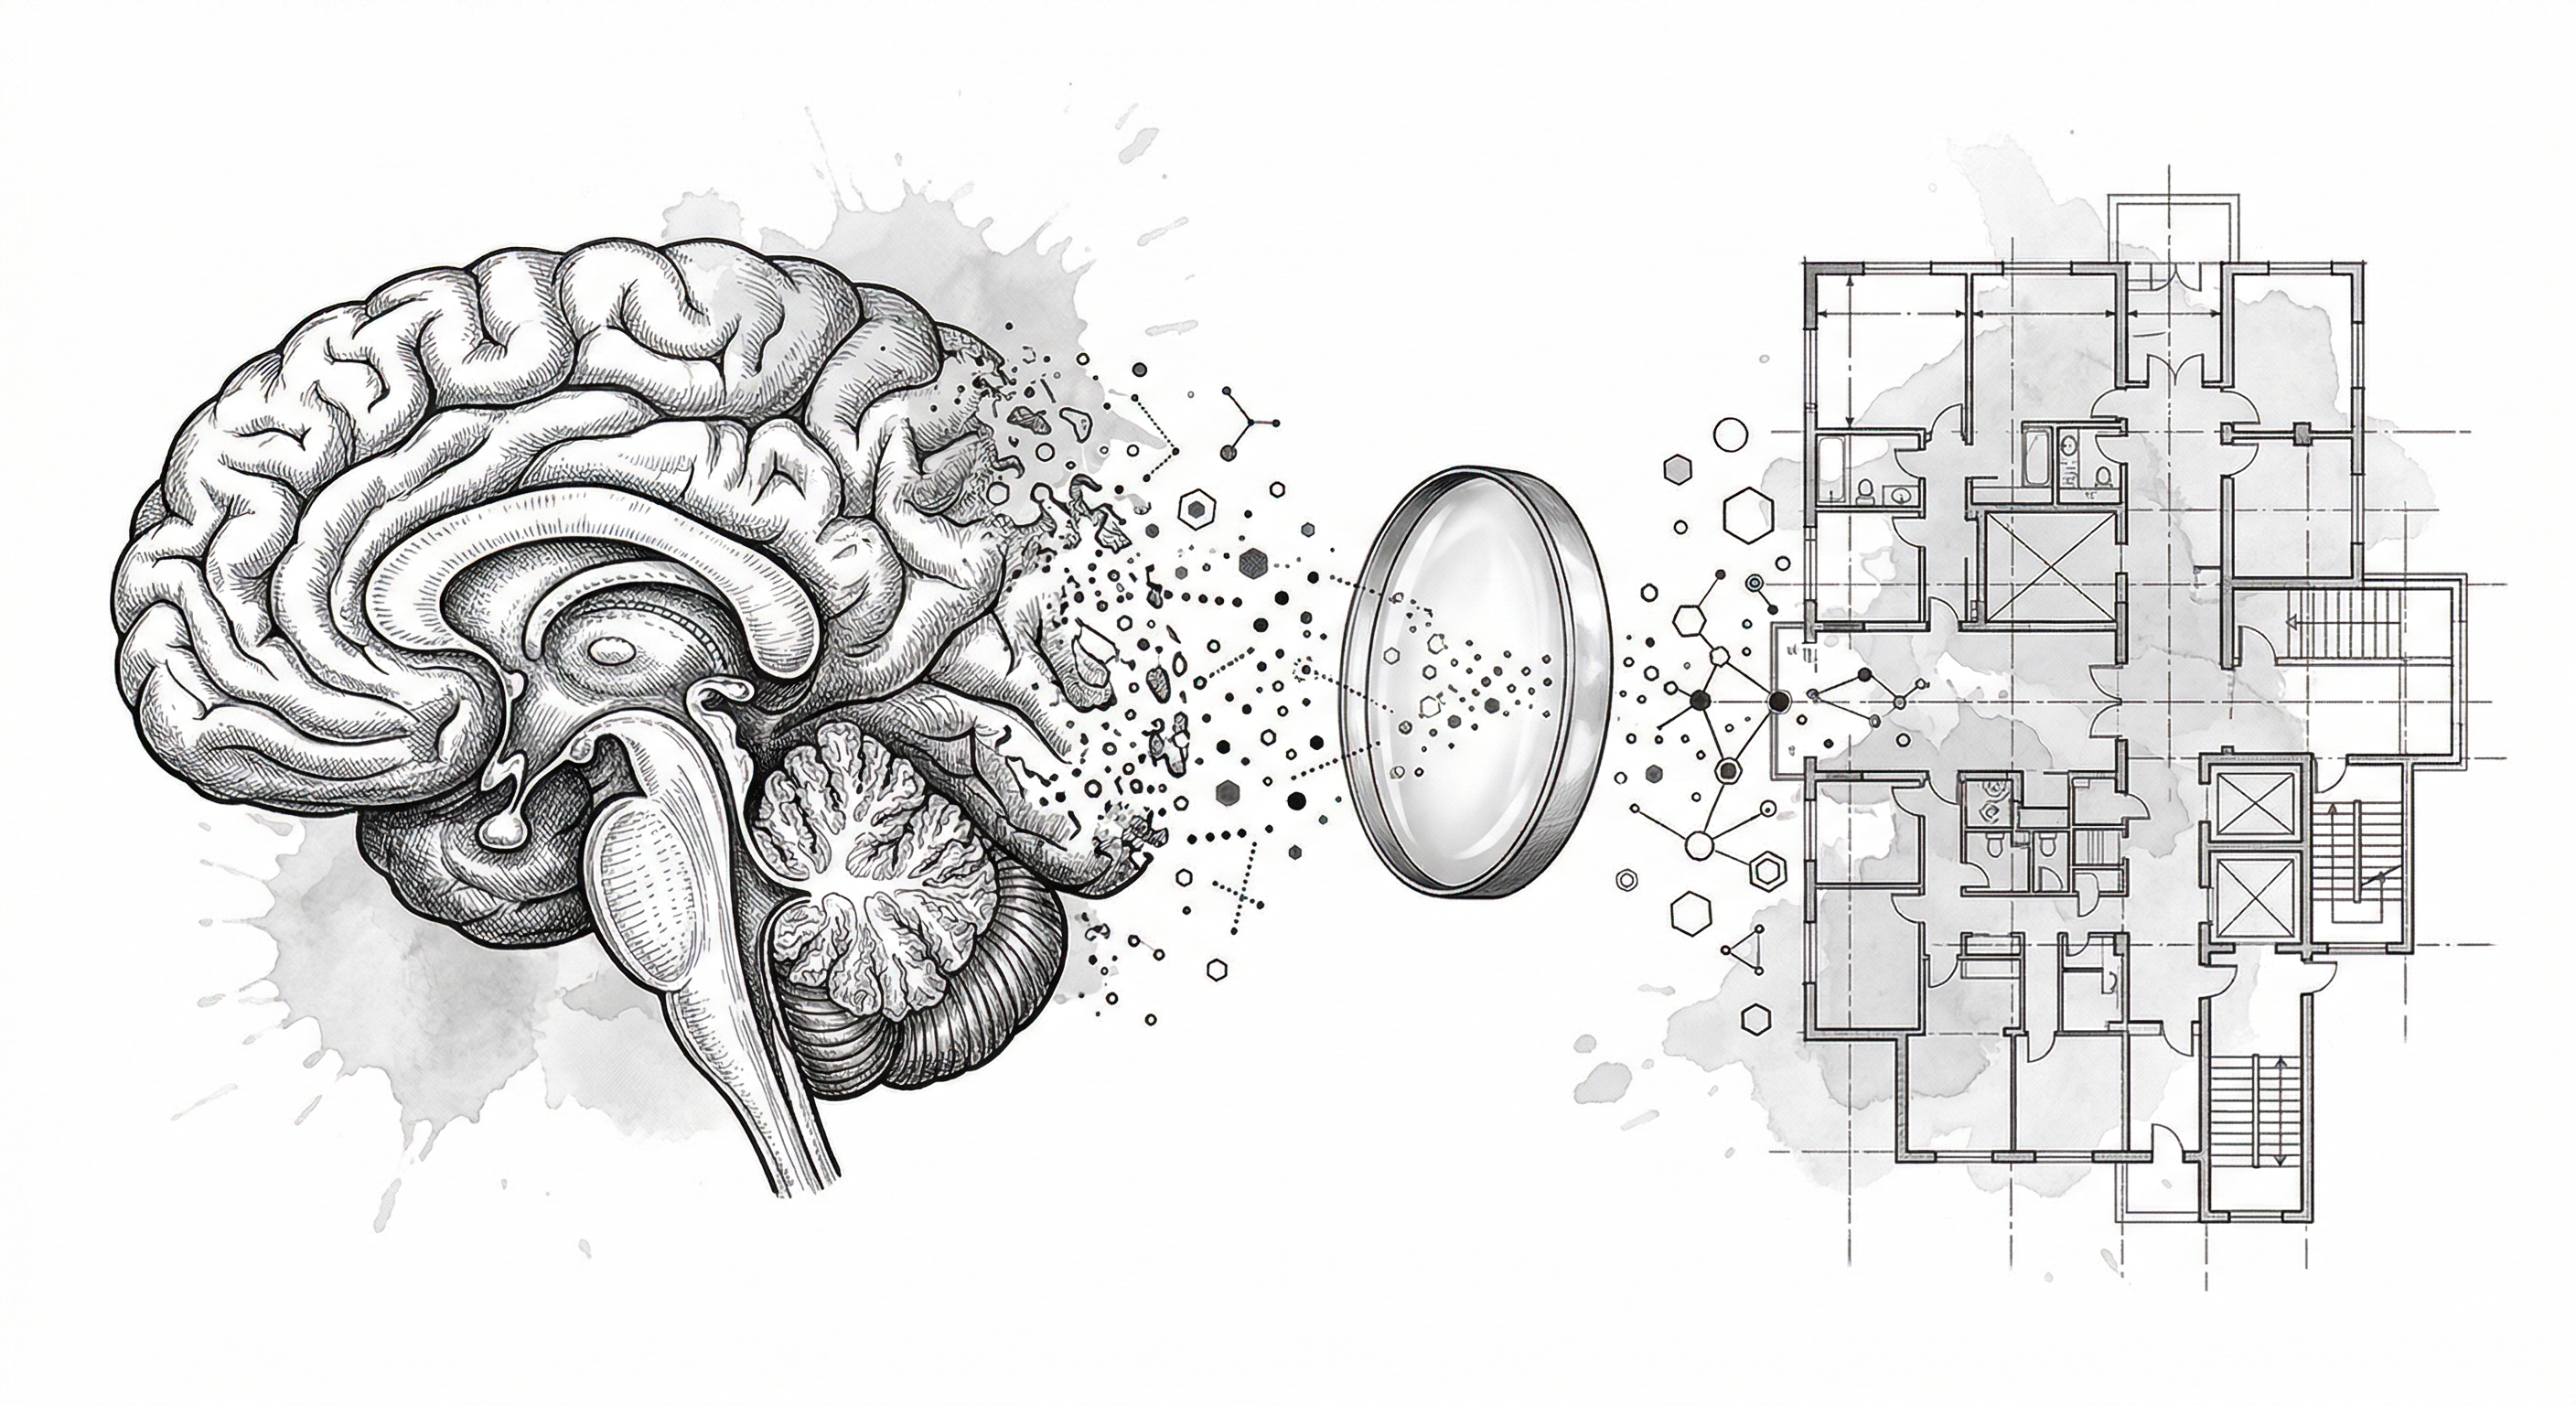
\includegraphics[width=0.75\textwidth]{images/frontcover_image.png}

    \vfill

    % --- Bottom: fulfilment, DOI, date ---
    {\small\textit{A thesis submitted in fulfilment of the requirements for the degree of\\
    Master of Enterprise IT Architecture (MSc)}}

    \vspace{0.2cm}
    {\small DOI: \href{https://doi.org/10.5281/zenodo.18367977}{10.5281/zenodo.18367977}}\\[0.1cm]
    {\small \today}
    \vspace{0.2cm}
\end{titlepage}

% Blank page after cover
\newpage\thispagestyle{empty}\mbox{}\newpage

% === FRONT MATTER WITH ROMAN NUMERALS ===
\pagenumbering{roman}

% Front matter page style: page numbers in header, no running title
\fancypagestyle{frontmatter}{%
  \fancyhf{}%
  \fancyhead[RO]{\thepage}%
  \fancyhead[LE]{\thepage}%
  \fancyfoot[LO]{\tiny\textcopyright~CC BY-SA 4.0~-- Version: \textit{v1.0 \builddate}}%
  \fancyfoot[RE]{\tiny\textcopyright~CC BY-SA 4.0~-- Version: \textit{v1.0 \builddate}}%
  \fancyfoot[RO]{\tiny Thiago A. de Faria~-- \url{https://github.com/thiagoavadore/thesis_2024-2026_antwerp_thesis_GenAIPracticeVacuum}}%
  \fancyfoot[LE]{\tiny Thiago A. de Faria~-- \url{https://github.com/thiagoavadore/thesis_2024-2026_antwerp_thesis_GenAIPracticeVacuum}}%
}
\pagestyle{frontmatter}
\global\currentheadrulewidth=0pt\relax
\global\currentfootrulewidth=0pt\relax

\onehalfspacing

% Front matter: executive summary, inner title, about, declaration,
% acknowledgments, TOC, LOF, LOT, abbreviations
% =============================================================================
% EXECUTIVE SUMMARY
% =============================================================================
\phantomsection
\section*{Executive Summary}
\addcontentsline{toc}{section}{Executive Summary}

Generative AI (GenAI) is changing how professionals work
\parencite{brynjolfsson_generative_2025, noy_experimental_2023}. Enterprise
Architecture (EA) practitioners have started using GenAI to develop Reference
Architectures (RAs), but no empirical research documents how they do so
\parencite{banh_affordance_genai_ea_2025}. Practitioners experiment in
isolation. They lack shared vocabulary, evaluation criteria, or validated
guidance. This study asks: \textit{What practices do EA practitioners adopt when
using GenAI for RA development, and how can these be systematized into guidance?}

We conducted a three-round Design-Oriented Delphi study
\parencite{skulmoski_delphi_2007} with seven to ten EA practitioners per
round. Round~1 (eight participants) collected asynchronous discovery workbooks.
Round~2 (ten participants) convened synchronous sessions to validate emerging
patterns. Round~3 (seven participants) refined verification heuristics and
critiqued a draft guidance artifact.

The panel identified seven practice categories that span RA development
activities. System/Codebase Analysis drew the strongest consensus. Stakeholder
Communication proved most context-dependent. Three shifts describe how GenAI
changes EA work. First, practitioners now spend more time checking GenAI outputs
than producing initial content. Second, the practitioner role moves from creator
to curator. Third, GenAI lets practitioners engage with topics beyond their
immediate expertise, which changes how roles interact.

Practitioners decide how much to trust GenAI based on the task at hand. The
dominant mental model treats GenAI as a junior colleague: capable, but requiring
supervision. Eight verification heuristics, organized in two tiers (structural
and domain), give practitioners concrete checks for validating outputs.
Table~\ref{tab:trust-spectrum-es} shows the resulting trust spectrum from full
delegation to full human retention.

\begin{table}[!ht]
    \centering
    \caption{Trust Spectrum for GenAI in RA Development}\label{tab:trust-spectrum-es}
    \begin{tabular}{|p{2.5cm}|p{5.5cm}|p{5.5cm}|}
        \hline
        \textbf{Trust Level} & \textbf{Task Type} & \textbf{Verification Approach} \\
        \hline
        Highest & Information compression: summaries, boilerplate, dependency graphs & Spot-check representative samples \\
        \hline
        High & Documentation drafts, concept explanation, test generation & Review structure and key claims \\
        \hline
        Medium & Code refactoring, common patterns, meeting synthesis & Verify against organizational standards \\
        \hline
        Medium-Low & Design trade-off exploration, technology recommendations & Cross-validate with primary sources \\
        \hline
        Low & Architecture decisions, novel business logic & Independent domain expert review \\
        \hline
        Very Low & Security-critical code, compliance assessment & Line-by-line verification \\
        \hline
        Lowest & Organizational judgment: politics, team dynamics, legal & Retain entirely; do not delegate \\
        \hline
    \end{tabular}
\end{table}

Two tensions cut across these findings. The first is a Ghost Architect dynamic:
when GenAI enables anyone to produce architectural artifacts, it becomes unclear
who is accountable. Organizations respond by shifting from periodic gate reviews
to continuous guardrails. The second is a competency decay risk: automating
foundational tasks (e.g., cold-start writing, exhaustive research) may erode the
learning process through which architectural expertise develops. Practitioners
counter this with deliberate practices such as AI-free design sessions and
independent-attempt-first protocols.

This study extends distributed cognition theory
\parencite{hutchins_cognition_1995}. GenAI acts as a new kind of cognitive
partner whose role is negotiated through practice, not predetermined by system
design. On the practical side, the study provides a taxonomy of GenAI practices
grounded in observable behavior. It shows where GenAI adds consistent value and
where its contribution depends on organizational context. The resulting guidance
artifact offers three levels of recommendation: directive (strong panel
consensus), contextual (moderate agreement, general recommendations), and
adaptive (high variability, requires organizational calibration).

\clearpage

% =============================================================================
% THESIS-COVER (AMS records page)
% =============================================================================
\newpage
\thispagestyle{empty}
\begin{center}
\vspace*{1.5cm}

{\Large\href{https://www.antwerpmanagementschool.be/}{\textsc{Antwerp Management School}}}\\[0.5cm]
{\Large\textsc{Master Thesis}}

\vspace{0.8cm}
\noindent\rule{0.7\textwidth}{0.4pt}

\vspace{0.7cm}
{\LARGE\bfseries From GenAI Practice Vacuum\\to Validated Guidance\par}
\vspace{0.4cm}
{\large A Delphi Study of AI-Augmented Reference Architecture Development\par}

\vspace{0.5cm}
\noindent\rule{0.7\textwidth}{0.4pt}

\vspace{1.5cm}

\begin{minipage}[t]{0.45\textwidth}
\raggedright
\textit{Author:}\\[0.3cm]
\href{https://www.linkedin.com/in/thiagodefarianl/}{\textsc{Thiago A. de Faria}}
\end{minipage}%
\hfill
\begin{minipage}[t]{0.45\textwidth}
\raggedleft
\textit{Supervisors:}\\[0.3cm]
Prof.\ Dr.\ Ing.\ \href{https://www.linkedin.com/in/jbfmulder/}{\textsc{Hans Mulder}}\\
\&\\
\href{https://www.linkedin.com/in/victorvanr/}{\textsc{Victor van Reijswoud}}, PhD\\
\&\\
\href{https://www.linkedin.com/in/edzob/}{\textsc{Edzo A.\ Botjes}} MSc.
\end{minipage}

\vspace{3cm}

\textit{A thesis submitted in fulfilment of the requirements for the degree of\\
Master of Enterprise IT Architecture (MSc)}

\vspace{0.5cm}
\today

\vspace{0.8cm}

\includegraphics[width=0.3\textwidth]{images/AMS_logo-lockup_black_rgb_150ppi.jpg}

\vfill
\end{center}

% Blank page after thesis-cover
\newpage\thispagestyle{empty}\mbox{}\newpage

% =============================================================================
% ABOUT / COLOPHON PAGE
% =============================================================================
\phantomsection
\section*{About}
\addcontentsline{toc}{section}{About}

{\footnotesize
\noindent From GenAI Practice Vacuum to Validated Guidance\\
- A Delphi Study of AI-Augmented Reference Architecture Development\\
Thesis content licensed under CC BY-SA 4.0 (\url{https://creativecommons.org/licenses/by-sa/4.0/})\\
Copyright \textcopyright\ 2024--2026 Thiago A. de Faria

\vspace{0.2cm}

\noindent\hspace{0.2cm}\textbf{Author}\\
\noindent\hspace{0.2cm}\textit{Name:} Thiago A. de Faria\\
\noindent\hspace{0.2cm}\textit{Email:} \href{mailto:thiagoavadore@gmail.com}{mailto:thiagoavadore@gmail.com}\\
\noindent\hspace{0.2cm}\textit{LinkedIn:} \href{https://www.linkedin.com/in/thiagodefarianl/}{linkedin.com/in/thiagodefarianl}\\
\noindent\hspace{0.2cm}\textit{ORCID:} \href{https://orcid.org/0009-0005-6631-4138}{0009-0005-6631-4138}

\vspace{0.2cm}

\noindent\hspace{0.2cm}\textbf{Supervisor}\\
\noindent\hspace{0.2cm}\textit{Name:} Prof.\ Dr.\ Ing.\ Hans Mulder\\
\noindent\hspace{0.2cm}\textit{Wikipedia:} \href{https://en.wikipedia.org/wiki/Hans_Mulder_(scientist)}{https://en.wikipedia.org/wiki/Hans\_Mulder\_(scientist)}\\
\noindent\hspace{0.2cm}\textit{LinkedIn:} \href{https://www.linkedin.com/in/jbfmulder/}{linkedin.com/in/jbfmulder}\\
\noindent\hspace{0.2cm}\textit{ORCID:} \href{https://orcid.org/0000-0002-3304-9711}{0000-0002-3304-9711}

\vspace{0.2cm}

\noindent\hspace{0.2cm}\textbf{Co-Supervisor}\\
\noindent\hspace{0.2cm}\textit{Name:} Edzo A.\ Botjes, MSc.\\
\noindent\hspace{0.2cm}\textit{LinkedIn:} \href{https://www.linkedin.com/in/edzob/}{linkedin.com/in/edzob}\\
\noindent\hspace{0.2cm}\textit{ORCID:} \href{https://orcid.org/0000-0003-0097-7375}{0000-0003-0097-7375}

\vspace{0.2cm}

\noindent\hspace{0.2cm}\textbf{Co-Supervisor}\\
\noindent\hspace{0.2cm}\textit{Name:} Victor van Reijswoud, PhD\\
\noindent\hspace{0.2cm}\textit{LinkedIn:} \href{https://www.linkedin.com/in/victorvanr/}{linkedin.com/in/victorvanr}\\
\noindent\hspace{0.2cm}\textit{ORCID:} \href{https://orcid.org/0009-0001-8594-2149}{0009-0001-8594-2149}

\vspace{0.2cm}

\noindent\hspace{0.2cm}\textbf{Thesis Project}\\
\noindent\hspace{0.2cm}GitHub \href{https://github.com/thiagoavadore/thesis_2024-2026_antwerp_thesis_GenAIPracticeVacuum}{github.com/thiagoavadore/thesis\_2024-2026\_antwerp\_thesis\_GenAIPracticeVacuum}

\vspace{0.2cm}

\noindent\hspace{0.2cm}\textbf{Publication References ID}\\
\noindent\hspace{0.2cm}DOI \href{https://doi.org/10.5281/zenodo.18367977}{10.5281/zenodo.18367977}

\vspace{0.2cm}

\noindent\hspace{0.2cm}\textbf{Keywords}\\
\noindent\hspace{0.2cm}Delphi Study, Design-Oriented Delphi, Distributed Cognition, EA Practice,\\
\noindent\hspace{0.2cm}Enterprise Architecture, GenAI, Generative AI, Large Language Models, LLM,\\
\noindent\hspace{0.2cm}Practice Theory, Reference Architecture, Software Architecture, Software Design,\\
\noindent\hspace{0.2cm}Target Architecture

\vspace{0.2cm}

\noindent\hspace{0.2cm}\textbf{Reference Style}\\
\noindent\hspace{0.2cm}This thesis is in compliance with APA Reference style version 7.\\
\noindent\hspace{0.2cm}\url{https://apastyle.apa.org/products/publication-manual-7th-edition}

\vspace{0.2cm}

\noindent\hspace{0.2cm}\textbf{Language}\\
\noindent\hspace{0.2cm}This thesis applies British English.

}

\clearpage

% =============================================================================
% FRONT COVER PAGE (no TOC entry, no PDF bookmark)
% =============================================================================
\thispagestyle{empty}
\section*{Front Cover}

{\footnotesize
\noindent The front cover is created by Thiago A. de Faria.

\vspace{0.3cm}

\noindent Image generated using Google Gemini with the prompt: ``Monochromatic grayscale academic illustration, no text, no letters, no words, no numbers. A detailed anatomical human brain on the left side, drawn in fine ink lines, partially dissolving into geometric particles and dots that drift rightward. These particles gradually reassemble into an abstract architectural blueprint floorplan on the right side, shown as precise technical line drawings of rooms, corridors, and structural elements. Between the brain and the blueprint, a translucent magnifying lens floats, refracting the particles passing through it, symbolizing verification and curation. Subtle watercolor ink splashes in light gray behind both elements. Small geometric shapes (circles, hexagons, connection nodes) scattered in the transition zone. Style: scientific illustration meets architectural drawing, similar to academic thesis cover art. White background, no color, purely grayscale ink and pencil aesthetic. High detail, scholarly tone.'', on 4 April 2026.
}

\clearpage

% =============================================================================
% DECLARATION OF AUTHORSHIP
% =============================================================================
\phantomsection
\section*{Declaration of Authorship}
\addcontentsline{toc}{section}{Declaration of Authorship}

I, Thiago A. de Faria, declare that this thesis titled, `From GenAI Practice Vacuum to Validated Guidance' and the work presented in it are my own. I confirm that:

\begin{itemize}
  \item This work was done wholly or mainly while in candidature for a research degree at Antwerp Management School.
  \item Where any part of this thesis has previously been submitted for a degree or any other qualification at Antwerp Management School or any other institution, this has been clearly stated.
  \item Where I have consulted the published work of others, this is always clearly attributed.
  \item Where I have quoted from the work of others, the source is always given. With the exception of such quotations, this thesis is entirely my own work.
  \item I have acknowledged all main sources of help.
  \item Where the thesis is based on work done by myself jointly with others, I have made clear exactly what was done by others and what I have contributed myself.
\end{itemize}

\vspace{2cm}

\noindent Signed: \rule{6cm}{0.4pt}

\vspace{1cm}

\noindent Date: \rule{6cm}{0.4pt}

% Blank page after declaration
\newpage\thispagestyle{empty}\mbox{}\newpage

% =============================================================================
% QUOTES PAGE
% =============================================================================

\vspace*{3cm}

\noindent\textit{`Historically, whenever a new AI paradigm has emerged, some AI researchers and many AI businesspeople have claimed ``that's it, we found the trick! Within 10 years we'll have machines that are smarter than humans.'' But they have been consistently over-optimistic. It's always harder than we think.'}

\hfill Yann LeCun (2025)

\vspace{1.2cm}

\noindent\textit{`A lot of what I'm spending my brain cycles on is machine learning ways to address safety: particularly how to design AI systems which eventually might be smarter than us, but that will behave well and not harm people.'}

\hfill Yoshua Bengio (2024)

\vspace{1.2cm}

\noindent\textit{`People are sufficiently clear and correct about the reasons for local decision making --- they know what information is available and how that information is used in deciding on action. But people often do not understand correctly what overall behavior will result from the complex interconnections of known local actions.'}

\hfill Jay W.\ Forrester (1995)

\vspace{1.2cm}

\noindent\textit{`A leader's job is to understand his people, understand their differences; optimize their interactions, their educations, their experiences.'}

\hfill Edward Deming (1991)

\vspace{1.2cm}

\noindent\textit{`The fundamental problem of communication is that of reproducing at one point either exactly or approximately a message selected at another point.'}

\hfill Claude Shannon (1948)

% Blank page after quotes
\newpage\thispagestyle{empty}\mbox{}\newpage

% =============================================================================
% ABSTRACT
% =============================================================================
\phantomsection
\addcontentsline{toc}{section}{Abstract}

\begin{center}
\vspace*{1.5cm}

{\large\href{https://www.antwerpmanagementschool.be/}{\textsc{Antwerp Management School}}}

\vspace{0.8cm}
{\LARGE\textit{Abstract}}

\vspace{0.6cm}
Faculty Enterprise Engineering\\
\href{https://www.antwerpmanagementschool.be/en/program/executive-master-digital-leadership-and-transformation/major-enterprise-it-architecture}{Executive Master Enterprise IT Architecture}

\vspace{0.4cm}
Master of Enterprise IT Architecture (MSc)

\vspace{0.6cm}
{\large\bfseries From GenAI Practice Vacuum to Validated Guidance}

\vspace{0.3cm}
by \textsc{Thiago A. de Faria}

\end{center}

\vspace{0.8cm}

Generative AI (GenAI) is rapidly integrating into professional knowledge work
and software development. Enterprise Architecture (EA) practitioners are using
GenAI to analyze systems, draft documentation, and develop Reference
Architectures (RAs). Yet no empirical research documents these emerging
practices, and no shared guidance exists.

This study uses distributed cognition as its integrating lens to examine how
cognitive work redistributes when GenAI enters RA development. We review the
literature on EA, RAs, GenAI capabilities, and distributed cognition to build a
conceptual model. We then conduct a three-round Design-Oriented Delphi study
with EA practitioners to validate emerging practices and produce a guidance
artifact.

The central finding is that GenAI acts as a new cognitive partner in the
distributed system of EA practice. Practitioners negotiate its role through
use: delegating information compression and first drafts, while retaining
architectural judgment and stakeholder decisions. The practitioner role shifts
from content creator to output curator. The resulting guidance artifact
systematizes these practices into directive, contextual, and adaptive
recommendations.

% Blank page after abstract
\newpage\thispagestyle{empty}\mbox{}\newpage

% =============================================================================
% DEDICATION PAGE
% =============================================================================

\vspace*{7cm}

\begin{center}
{\large\textit{Dedicated to Isabela, the love of my life,\\and to our children Nina and Liam, who fill it with meaning}}
\end{center}

% Blank page after dedication
\newpage\thispagestyle{empty}\mbox{}\newpage

% =============================================================================
% ACKNOWLEDGMENTS
% =============================================================================
\phantomsection
\section*{Acknowledgments}
\addcontentsline{toc}{section}{Acknowledgments}

\hspace{\parindent}I would like to thank my family (Isabela, Nina and Liam) for their support
during these almost two years. Travelling to Antwerp meant being away from
little kids and leaving all the extra work to Isabela. Knowing that I had
nothing to worry about at home is a priceless gift. Furthermore, I would like
to thank the following people.

\vspace{1em}
\noindent\textbf{Antwerp Management School}
\vspace{0.5em}

\noindent Thanks to AMS for providing the inspiration, content and discussions that
boosted my learning experience. I have the utmost respect for my supervisors
Prof.\ Dr.\ Ing.\ Hans Mulder, Victor van Reijswoud PhD and Edzo A.\ Botjes
MSc, for the sage advice and effort they put into guiding this work. Your
patience and guidance throughout this journey are the greatest show of trust I
could have experienced.

\vspace{1em}
\noindent\textbf{The Delphi Study Participants}
\vspace{0.5em}

\noindent A remarkably diverse group in nationalities, work experience and job titles
helped me enormously during the Delphi Study. Due to anonymity I cannot reveal
their names, but they know who they are. The extensive discussions, arguments
and counter-arguments shaped this research in ways I could not have anticipated.
In such a fast-paced subject as the adoption of GenAI tools in the tech world,
you all recognized the unknowns and showed the willingness to adapt and revise
your opinions. Thank you!

\vspace{1em}
\noindent\textbf{All the AI Builders Out There}
\vspace{0.5em}

\noindent We live in unprecedented times. I would like to thank the practitioners and
builders out there who are pushing software development to new standards and
heights: open-source coders releasing tools that are changing the world, and
researchers advancing new methodologies, AI safety and ethics. I have been
working in the IT industry for 20 years, and what has happened in the last
three years displays the disruptive (sorry for using this word) power that
technology has. It is up to us, builders, leaders and researchers, to discuss,
iterate and ask for help. The consequences of AI pervasiveness, the ethical
discussions, the impact on society and on people's practice and identity cannot
be forgotten. I am glad the majority of AI builders out there are building in
the open.

% Blank page after acknowledgments
\newpage\thispagestyle{empty}\mbox{}\newpage

% =============================================================================
% TABLE OF CONTENTS, LIST OF FIGURES, LIST OF TABLES
% =============================================================================
\phantomsection
\addcontentsline{toc}{section}{Table of Contents}
\section*{Contents}
\etocstandardlines          % Use standard LaTeX TOC formatting for global TOC
\tableofcontents
% Re-enable custom formatting for local mini-TOCs
\etocsetstyle{subsection}
  {\begin{list}{}{\setlength{\leftmargin}{0.5in}\setlength{\itemsep}{0pt}\setlength{\parsep}{0pt}}}
  {\item}
  {\makebox[2.5em][l]{\etocnumber}\etocname\nobreak\leaders\hbox to 0.5em{\hss.\hss}\hfill\nobreak\makebox[2em][r]{\etocpage}}
  {\end{list}}
\clearpage

\phantomsection
\listoffigures
\addcontentsline{toc}{section}{List of Figures}
\clearpage

\phantomsection
\listoftables
\addcontentsline{toc}{section}{List of Tables}
\clearpage

% =============================================================================
% LIST OF ABBREVIATIONS
% =============================================================================
\phantomsection
\section*{List of Abbreviations}
\addcontentsline{toc}{section}{List of Abbreviations}

\begin{longtable}{@{} l l @{}}
AMS   & Antwerp Management School \\
APA   & American Psychological Association \\
API   & Application Programming Interface \\
CLT   & Cognitive Load Theory \\
DCog  & Distributed Cognition \\
EA    & Enterprise Architecture \\
GenAI & Generative Artificial Intelligence \\
GSS   & Group Support System \\
LLM   & Large Language Model \\
MRQ   & Main Research Question \\
RA    & Reference Architecture \\
sRQ   & Sub-Research Question \\
TOGAF & The Open Group Architecture Framework \\
\end{longtable}
\clearpage

% Blank page before main content
\newpage\thispagestyle{empty}\mbox{}\newpage


% === MAIN CONTENT WITH ARABIC NUMERALS ===
\pagenumbering{arabic}
\pagestyle{fancy}
\global\currentheadrulewidth=0.4pt\relax
\global\currentfootrulewidth=0.4pt\relax
\fancyhead[RE]{\small\leftmark}
\fancyhead[LO]{\small\rightmark}

% Larger section titles for main body (sections 01-08) and appendices
\titleformat{\section}
  {\normalfont\fontsize{16}{19}\bfseries}{\thesection}{1em}{#1}
\titlespacing{\section}{0pt}{12pt}{12pt}

\titleformat{\subsection}
  {\normalfont\fontsize{12}{14}\bfseries}{\thesubsection}{1em}{#1}
\titlespacing{\subsection}{0pt}{12pt}{12pt}

% Section/subsection marks for running headers + first-page style
\renewcommand{\sectionmark}[1]{%
  \markboth{Section \thesection.\ \ #1}{}%
  \thispagestyle{sectionfirst}%
  \global\currentheadrulewidth=0pt\relax
  \global\currentfootrulewidth=0pt\relax}
\renewcommand{\subsectionmark}[1]{\markright{\thesubsection\ \ #1}}
\AddToHook{shipout/after}{%
  \global\currentheadrulewidth=0.4pt\relax
  \global\currentfootrulewidth=0.4pt\relax}

\section{Introduction}\label{sec:introduction}

This section establishes the research problem and derives the research
questions that guide this study. We begin by situating Generative AI (GenAI)
in professional practice, then examine its implications for Enterprise
Architecture (EA) and Reference Architecture (RA) development. Two gaps
emerge: a practice gap, where no empirical research documents how EA
practitioners integrate GenAI into RA development, and a guidance vacuum,
where practitioners experiment in isolation without shared frameworks.

The \textit{Theoretical Background} (Section~\ref{sec:theoretical-background}) provides the theoretical foundation
on EA, RAs, GenAI capabilities, and distributed cognition.
The \textit{Conceptual Model} (Section~\ref{sec:conceptual-model}) presents the conceptual model that frames
the investigation. The \textit{Methodology} (Section~\ref{sec:methodology}) explains the Design-Oriented
Delphi methodology used to answer the research questions. The following
subsections detail this investigation:

\localtableofcontents\clearpage

\subsection{The emergence of Generative AI in Professional Practice}

Since the public release of ChatGPT in November 2022, Generative AI (GenAI) has
become a routine part of professional work
\parencite{brynjolfsson_generative_2025}. ChatGPT reached 100 million users
within two months \parencite{hu_chatgpt_2023}. By 2025, 84\% of developers use
AI coding tools, up from 76\% one year earlier
\parencite{stack_overflow_2024, stack_overflow_2025}, and 75\% of knowledge
workers across 31 countries report using AI regularly
\parencite{microsoft_wti_2025}. Yet adoption has outpaced preparation: 83\% of
workers are self-taught in AI, and only 52\% of senior leaders have deployed
formal AI training \parencite{ey_agentic_2025}.

The infrastructure behind this adoption is large and growing. In 2025, the major
US hyperscalers (Amazon, Microsoft, Google, and Meta) are collectively investing
approximately \$320 billion in AI infrastructure, more than 1\% of US GDP
\parencite{understanding_ai_2025}. Microsoft alone has committed \$80 billion to
data center construction in fiscal year 2025 \parencite{cnbc_tech_2025}. The
\textcite{iea_energy_2025} projects that global electricity consumption from
data centers will more than double by 2030, reaching 945 TWh (equivalent to
Japan's entire current consumption). In the United States, data centers are
forecast to account for almost half of electricity demand growth between 2024
and 2030 \parencite{iea_energy_2025}. \textcite{mckinsey_cost_2025} estimates
the total cost to scale AI data center infrastructure at \$7 trillion. These
investments have multi-decade lifespans. The practical question is not whether
GenAI will persist, but how practitioners should adapt their work to it.

\subsection{Reference Architecture Development}

Enterprise Architecture (EA) is a discipline that aligns organizational
strategy, processes, and IT infrastructure
\parencite{lankhorst_enterprise_2017}. EA practitioners analyze, design, and
govern how organizations structure their technology ecosystems
\parencite{the_open_group_togaf_2022}. Among their outputs are Reference
Architectures (RAs): documented patterns and templates for system
implementations \parencite{cloutier_concept_2010}. RAs enable reuse across
projects, reduce design risk, promote interoperability, and serve as knowledge
repositories for stakeholder communication
\parencite{cloutier_concept_2010, angelov_framework_2012}.

In practice, RA development involves more than formal EA titles.
\textcite{kotusev_enterprise_2018} showed that EA artifacts are built
collaboratively by architects, business executives, analysts, and developers.
Solution architects, platform engineers, and senior developers routinely shape
these artifacts through daily work. Developing RAs requires analyzing existing
systems, identifying patterns, engaging stakeholders, and synthesizing technical
and business considerations.

GenAI is already entering this work. Developer tools powered by GenAI are
shaping architectural patterns from the bottom up, through code generation,
design suggestions, and automated documentation, often before formal EA
governance becomes aware
\parencite{peng_impact_2023, tabarsi_llms_reshaping_se_2025}. This makes
understanding how practitioners use GenAI in RA development urgent.

\subsection{The Practice Gap}

No empirical research documents how EA practitioners integrate GenAI into RA
development\footnote{ EBSCO host advanced search conducted on June 8, 2025,
    resulted in 0 publications using the query: ((enterprise architecture OR ea
    practice) AND (gen ai OR generative artificial intelligence OR llm OR large
    language models)) AND SO (MIS Quarterly Executive OR Information Systems
    Research OR Journal of the Association for Information Systems OR European
    Journal of Information Systems) Filters applied: peer-reviewed articles,
    publication date from January 1, 2020, to June 8, 2025
}. Research in adjacent fields (software engineering, management consulting,
general knowledge work) shows that GenAI changes professional practice
\parencite{peng_impact_2023, dellacqua_navigating_2023, noy_experimental_2023},
but EA remains unstudied
\parencite{banh_affordance_genai_ea_2025, ettinger_ea_dynamic_capability_2025}.

This gap matters for three reasons. First, EA work involves both technical and
social dimensions. Practitioners navigate organizational politics, synthesize
diverse perspectives, and create artifacts that must resonate with multiple
stakeholders. How GenAI tools, primarily trained on technical content, interact
with this sociotechnical reality is unknown. Second, RA development is
knowledge-intensive. It requires capturing, synthesizing, and codifying
architectural knowledge. GenAI's capabilities for pattern recognition and
content generation could change how this knowledge work is done, but no evidence
documents whether or how. Third, research in other domains shows that
professionals restructure their work practices around AI rather than simply
using it as a faster tool \parencite{noy_experimental_2023,
tankelevitch_metacognitive_2024, dellacqua_navigating_2023}. Whether EA
practitioners are experiencing similar changes is unexamined.

\subsection{The Guidance Vacuum}

Practitioners who experiment with GenAI in EA work do so without shared
vocabulary, evaluation criteria, or validated guidance. Specifically, they lack:

\begin{enumerate}
    \item Evidence of which practices work for GenAI use in EA
          \parencite{banh_affordance_genai_ea_2025}.
    \item Frameworks for judging when GenAI helps versus hinders architectural
          activities \parencite{esposito_genai_architecture_2026}.
    \item Guidance on managing the risks of human-AI collaboration in EA,
          particularly over-reliance \parencite{dellacqua_navigating_2023}.
\end{enumerate}

Without shared guidance, each practitioner reinvents the wheel
\parencite{feldman_theorizing_2011}. Emerging practices cannot consolidate into
reliable routines, and organizations risk both missed opportunities and quality
problems \parencite{dellacqua_navigating_2023}.

\subsection{Research Opportunity}

In our view, these gaps call for an investigation into how EA practitioners
develop new practices as they integrate GenAI into RA development. This is not
a tool-adoption study; Section~\ref{subsec:framework-dynamics} develops this argument further. Research in adjacent domains shows that professionals
reshape their work around AI capabilities rather than bolting AI onto existing
workflows \parencite{noy_experimental_2023, dellacqua_navigating_2023}.

We focus on RA development because it is a central EA activity
\parencite{cloutier_concept_2010, the_open_group_togaf_2022} that spans the
full range of architectural work: analysis, synthesis, and documentation. If
GenAI changes how RAs are developed, the effects will extend to governance,
implementation, and knowledge management. Beyond documenting current practices,
the aim is to develop practical guidance that supports EA practitioners in
navigating this change.

In sum, GenAI is a structural shift in professional knowledge work. RA
development is knowledge-intensive sociotechnical work for which no empirical
guidance exists. Developer-level GenAI use is already shaping architectural
artifacts before formal EA governance becomes aware. The following subsections
translate this problem into research questions.

\subsection{Deriving the Research Questions}\label{sec:research-question}

The introduction identified two gaps. A \emph{practice gap}: no empirical
research documents how EA practitioners integrate GenAI into RA development.
And a \emph{guidance vacuum}: practitioners experiment in isolation, without
shared frameworks or vocabulary. These gaps call for research that both
documents emerging practices and produces actionable guidance.

\subsection{Main Research Question}

\begin{quote}
\textit{What practices do EA practitioners adopt when using GenAI for RA development,
and how can these be systematized into guidance?}
\end{quote}

The first part of this question targets practice discovery. The second targets
guidance development. This reflects a practice-based perspective: technology
integration is not a one-time event but an ongoing process shaped by how people
actually use tools in context \parencite{feldman_theorizing_2011,
orlikowski_using_2000}. GenAI and EA practice shape one another. Practitioners
adapt their workflows to GenAI, while GenAI outputs depend on practitioner
expertise and organizational context \parencite{orlikowski_sociomaterial_2007}.
Answering this question requires a methodology that captures both current
practices and the ambition to produce practical guidance.

\subsection{Sub-Questions}\label{subsec:sub-questions}

Four sub-questions decompose the main RQ into a progression from description
through analysis and interpretation to design:

\vspace{0.5em}
\noindent\textbf{sRQ1:} What GenAI practices are EA practitioners currently using when developing RAs?

\vspace{0.5em}
\noindent\textbf{sRQ2:} What changes to EA practice are EA practitioners experiencing when RAs are developed using GenAI?

\vspace{0.5em}
\noindent\textbf{sRQ3:} How do EA practitioners make sense of impacts and trade-offs when adopting GenAI for RA development?

\vspace{0.5em}
\noindent\textbf{sRQ4:} How should effective GenAI practices for RA development be systematized into guidance for EA practitioners?

\vspace{0.5em}
\noindent Throughout these questions, ``EA practitioners'' refers broadly to all
professionals contributing to RA development, as formally defined in
Section~\ref{sec:theoretical-background}.

\subsection{Sub-Question Progression}

The four sub-questions follow a deliberate sequence. sRQ1 is
\emph{descriptive}: it maps which GenAI practices EA practitioners currently
use. sRQ2 is \emph{analytical}: it examines how these practices change existing
EA work. sRQ3 is \emph{interpretive}: it surfaces how practitioners weigh the
impacts and trade-offs they experience.

sRQ4 differs from the first three. Where sRQ1 through sRQ3 investigate what
\emph{is}, sRQ4 asks what \emph{should be}. It synthesizes empirical findings
into a guidance artifact that practitioners can use
\parencite{gregor_positioning_2013}. This shift from empirical inquiry to
artifact construction is characteristic of the Design-Oriented Delphi
methodology adopted in this study (Section~\ref{sec:methodology}).

\clearpage
\section{Theoretical Background}\label{sec:theoretical-background}

\subsection*{Introduction}

This section defines the five constructs that ground the study: Enterprise
Architecture (EA), EA practitioners, EA practice, Reference Architectures (RAs),
and Generative AI (GenAI). It then introduces distributed cognition as the
theoretical lens that connects them. The theoretical background from this
section is used in the construction of the conceptual model in
the \textit{Conceptual Model} (Section~\ref{sec:conceptual-model}). The following subsections detail these
foundations:

\localtableofcontents\clearpage

\subsection{Enterprise Architecture}\label{subsec:enterprise-architecture}

Enterprise Architecture has roots in IBM's Business Systems Planning methodology
of the 1960s \parencite{kotusev_enterprise_2018} and emerged as a distinct
discipline with \textcite{zachman_zachman_1987}'s framework. After nearly four
decades, the field still lacks a shared definition.
\textcite{saint-louis_investigation_2019} found that EA means different things
to different people, with definitions varying across theoretical lenses and
organizational contexts.

\textcite{the_open_group_togaf_2022} defines EA as the practice of analyzing,
designing, planning, and implementing enterprise-level analysis in service of
business strategy. \textcite{lankhorst_enterprise_2017} presents EA as an
integrated set of principles, methods, and models for designing an enterprise's
organisational structure, business processes, information systems, and
infrastructure. The first definition treats EA as an active practice; the second
treats it as both process and product.

\textcite{saint-louis_investigation_2019} identified a useful distinction: EA
as a noun versus EA as a verb. As a noun, EA refers to deliverables, models, and
artifacts. As a verb, it refers to the practice and process of architecting.
This distinction matters for this study because GenAI may affect both what
practitioners produce and how they produce it.

The lack of definitional consensus has practical consequences.
\textcite{kotusev_enterprise_2018} notes that EA frameworks offer vague,
inconsistent, and conflicting recommendations, creating problems for
organizations trying to implement EA. Some view EA as primarily IT-focused;
others emphasize business-IT alignment or enterprise-wide transformation
\parencite{gartner_gartner_2008, ross_enterprise_2006}.

In our view, EA is best understood as the sociotechnical practice of analyzing,
designing, and governing an enterprise's structures, processes, and technology
to enable strategic alignment. This working definition bridges the noun and verb
perspectives: EA produces tangible artifacts (models, standards, principles)
through an ongoing practice of stakeholder negotiation, technical design, and
organizational adaptation
\parencite{saint-louis_investigation_2019, the_open_group_togaf_2022, lankhorst_enterprise_2017}.

\subsubsection{Historical Evolution}\label{subsubsec:ea-history}

EA's origins are commonly traced to \textcite{zachman_zachman_1987}'s ``A
Framework for Information Systems Architecture.'' This work introduced multiple
perspectives and abstraction levels for describing enterprises. Zachman
established the principle that a single complex object can be described in
multiple ways, depending on the purpose and type of description required
\parencite{zachman_zachman_1987}. Early EA was largely understood through
an engineering metaphor, with practitioners viewing themselves as technical
specialists designing optimal IT solutions \parencite{spewak_enterprise_1993}.

The discipline shifted in the 2000s. \textcite{ross_enterprise_2006}
repositioned EA as the organizing logic that aligns core business processes and
IT infrastructure with a firm's integration and standardization requirements
\parencite{ross_enterprise_2006}. This moved
EA from documentation toward strategic capability. The Open Group's TOGAF
framework, first published in 1995, gained prominence through successive
revisions \parencite{the_open_group_togaf_2022}.

More recently, \textcite{kotusev_enterprise_2018} challenged many assumptions
about EA in practice. He argues that the current conceptualization rests on
anecdotal stories and wishful thinking rather than empirical evidence. Through
case study research, he showed that successful EA practices diverge from
mainstream prescriptions. Rather than following a linear path toward maturity,
EA practices adapt to organizational contexts, with successful implementations
often bearing little resemblance to framework prescriptions.

\textcite{saint-louis_investigation_2019} similarly notes that despite decades
of development, EA still lacks common understanding. EA continues to evolve,
with practitioners and researchers still working out its boundaries and methods.

\subsubsection{EA as Sociotechnical Practice}\label{subsubsec:ea-sociotechnical}

EA is not purely technical work. \textcite{saint-louis_investigation_2019}
identified three contexts within which EA operates, each combining technical and
social dimensions:

\begin{enumerate}
      \item Technological: IT infrastructure, systems integration, and technical
            optimization
      \item Socio-Technological: stakeholder participation, communication, and
            collaborative decision-making
      \item Eco-Technological: ecosystem relationships, compliance requirements,
            and external standards
\end{enumerate}

EA practice requires integrating both technical and social considerations in
specific organizational settings. \textcite{gregor_enterprise_2007} demonstrated
through case studies that effective EA development requires stakeholder
participation, with solutions achieved through communication, negotiation, and
collaboration. \textcite{lankhorst_enterprise_2017} similarly characterizes EA
as a holistic approach to organisational design, where multiple
domains (organization, information, systems, products, processes, and
applications) intersect. This sociotechnical character is why GenAI integration
in EA is not simply a tool-adoption question.

\subsection{EA Practitioners and EA Practice}\label{subsec:ea-practitioners}

\subsubsection{EA Practitioners: Roles and Evolution}\label{subsubsec:ea-roles}

EA practitioners are the professionals who develop, maintain, and govern
enterprise architectures
\parencite{kotusev_enterprise_2018, the_open_group_togaf_2022}.
\textcite{kotusev_enterprise_2018} notes that EA artifacts are developed not
only by dedicated architects but also by business executives, business analysts,
project managers, and software developers. EA practice therefore extends beyond
formal ``Enterprise Architect'' job titles.

\textcite{saint-louis_investigation_2019} identified three practitioner
archetypes:

\begin{enumerate}
      \item \textbf{Specialists}: technical experts focused on selecting optimal
            solutions for organizational needs
            \parencite{saint-louis_investigation_2019}.
      \item \textbf{Integrators}: practitioners who prioritize stakeholder
            participation and motivation in the decision-making process
            \parencite{saint-louis_investigation_2019}. They bridge technical and
            business domains through negotiation.
      \item \textbf{Facilitators}: professionals who view IT implementation and
            stakeholder engagement as inseparable from broader organizational
            adaptation \parencite{saint-louis_investigation_2019}.
\end{enumerate}

In practice, EA practitioners shift between these roles depending on the
situation. \textcite{land_enterprise_2009} observe that effective architects
need competencies spanning technical expertise, communication, leadership, and
political acumen. \textcite{van_steenbergen_maturity_2011} shows that EA
effectiveness depends on maturity across multiple dimensions, not technical
capability alone.

Our position is that ``EA practitioners'' in this research encompasses all
professionals who contribute to the development and governance of architectural
artifacts: enterprise architects, solution architects, platform engineers, data
architects, and senior software engineers who shape RAs through their daily
work. \textcite{kotusev_enterprise_2018}'s finding of distributed authorship
supports this broader scope.

\subsubsection{EA Practice: Beyond Frameworks}\label{subsubsec:ea-practice-frameworks}

We understand EA practice, following \textcite{feldman_theorizing_2011}, as the
recurrent patterns of action through which practitioners accomplish
architectural work. These practices are sociomaterial accomplishments
\parencite{orlikowski_sociomaterial_2007}: they involve both human actors and
technological artifacts.

\textcite{kotusev_enterprise_2018}'s empirical research revealed four
disconnects between formal EA frameworks and actual practice.
\textcite{ross_enterprise_2006}, \textcite{fonstad_n_o_transforming_2006}, and
\textcite{ahlemann_strategic_2012} corroborate these findings:

\begin{enumerate}
      \item \textbf{Incremental Development}: EA artifacts evolve gradually
            through organizational learning, not all at once
            \parencite{kotusev_enterprise_2018}.
      \item \textbf{Distributed Authorship}: Business executives are actively
            involved, sometimes leaving enterprise architects in a secondary
            facilitator role
            \parencite{kotusev_enterprise_2018, ross_enterprise_2006}.
      \item \textbf{Broad Application}: EA applications extend beyond strategic
            initiatives to address local requirements, unforeseen demands, and
            unplanned deviations \parencite{fonstad_n_o_transforming_2006}.
      \item \textbf{Process Integration}: Successful EA integrates with
            strategic, project, and operations management
            \parencite{ahlemann_strategic_2012}.
\end{enumerate}

The point is that EA work happens through dynamic interactions among
practitioners, tools, and organizational structures. As
\textcite{feldman_theorizing_2011} argue, understanding practice means examining
how activities are generated and operate within different contexts and over time
\parencite[p.~1241]{feldman_theorizing_2011}.

\subsection{Reference Architectures and Their Lifecycle}\label{subsec:reference-architectures}

\textcite{cloutier_concept_2010} define a Reference Architecture (RA) as an
authoritative knowledge source for a specific domain that guides and constrains
how concrete architectures and solutions are instantiated.
\textcite{angelov_framework_2012} complement this by characterizing RAs as
generic architectures for a class of information systems, designed to provide
standardization, interoperability, and reuse. RAs serve four functions: they
capture proven architectural patterns, control complexity through abstraction,
promote common understanding among stakeholders, and reduce risk through reuse
of validated designs \parencite{cloutier_concept_2010}.

\textcite{cloutier_concept_2010} describe how RAs are built from proven
architectures of past and existing products yet provide guidance for future
implementations. RAs must therefore evolve with technological change and
organizational learning. However, the literature does not present a unified view
of the RA lifecycle. The following subsections review five perspectives, then
synthesize them into an operational definition and sensitizing lifecycle model.
This model serves as a structuring device for the Delphi study: Round~1
participants position their practices within the lifecycle phases, providing
empirical validation of its utility (Section~\ref{sec:methodology}).

\subsubsection{Perspective 1: Continuous Development Cycle}

\textcite{cloutier_concept_2010} present a development cycle showing the
relationship between existing architectures, RA patterns, and new
implementations. In their view, RAs should evolve continuously because
organizational needs, technologies, and standards change. This requires active
maintenance and refactoring \parencite{cloutier_concept_2010}. They stress that
the Chief Architect (business plus technical) owns the RA and that business
sponsorship is a prerequisite.

\subsubsection{Perspective 2: Evolution and Transformation}

\textcite{angelov_framework_2012} focus on how RAs evolve over time. Using
their classification framework (which categorizes RAs by context, goal, and
scope), they note that an RA may shift categories as its environment changes or
its organizational goal evolves. Examples of evolution paths include:

\begin{itemize}
      \item A preliminary RA transforming into a classical architecture when the
            domain matures
      \item Evolution from facilitation to standardization as organizational
            needs change
      \item Expansion from single organization scope to multiple organizations
\end{itemize}

To remain usable, an RA must be adapted to reflect such changes
\parencite{angelov_framework_2012}.

\subsubsection{Perspective 3: Creation and Application Context}

Creating RAs involves analyzing existing systems, identifying commonalities and
variations, and abstracting from implementation specifics
\parencite{angelov_framework_2012}. Application requires careful attention to
context, since the generic nature of RAs leads to less defined design and
application boundaries. \textcite{cloutier_concept_2010} describe the challenge
of making RAs accessible to multiple stakeholders (engineers, business managers,
customers) while keeping them generic enough for broad reuse yet concrete enough
to be actionable. This tension between abstraction and concreteness cannot be
resolved through technical means alone. It requires ongoing negotiation with the
stakeholders who must interpret and apply the guidance.

\subsubsection{Perspective 4: Stakeholder Engagement and Validation}

The literature emphasizes intensive stakeholder involvement throughout the RA's
existence. \textcite{ross_j_w_maturity_2004} found that developing an
architectural vision required approximately sixty meetings of the executive
team, illustrating the collaboration that architectural work demands.
\textcite{angelov_framework_2012} note that RA quality can be measured by its
success in fulfilling its goals, which requires ongoing validation through
implementation and feedback.

\subsubsection{Perspective 5: Ongoing Refinement}

Rather than following a linear lifecycle, the literature suggests RAs exist in a
state of continuous adaptation. \textcite{cloutier_concept_2010} explain that
RAs must be actively managed to ensure they are updated based on evolving
standards, emerging technology, changing stakeholder requirements, and maturing
business needs. The RA lifecycle is an ongoing process of refinement, not a
sequence of phases.

\subsubsection{Operational Definition for This Research}

The five perspectives can be summarized as follows:

\begin{enumerate}
      \item \textbf{Continuous Development Cycle}: RAs require active
            maintenance, not one-time creation
            \parencite{cloutier_concept_2010}.
      \item \textbf{Evolution and Transformation}: RAs shift across categories
            as technology, experience, and goals change
            \parencite{angelov_framework_2012}.
      \item \textbf{Creation and Application Context}: RA design must balance
            abstraction for reuse with concreteness for implementation
            \parencite{angelov_framework_2012, cloutier_concept_2010}.
      \item \textbf{Stakeholder Engagement}: Architectural work demands
            extensive multi-stakeholder collaboration
            \parencite{ross_j_w_maturity_2004, angelov_framework_2012}.
      \item \textbf{Ongoing Refinement}: RAs exist in continuous adaptation
            driven by implementation experience
            \parencite{cloutier_concept_2010}.
\end{enumerate}

RA work extends well beyond initial creation. For this study, Reference
Architecture encompasses templates, standards, patterns, governance documents,
blueprints, and domain models used as reference for downstream architectural
design, regardless of formality level. Project-specific solution architectures
fall outside this scope, unless they are reused as reference for other projects,
at which point they function as RAs.

This broad scope reflects how practitioners engage with RAs in practice. RA work
encompasses creating, reading, absorbing, contextualizing, validating,
communicating, governing, and evolving architectural artifacts.
\textcite{cloutier_concept_2010} describe a continuous development cycle in
which RAs require active organizational management.
\textcite{angelov_framework_2012} note that RAs must evolve to reflect
changes in technology, experience, and goals.

\subsubsection{Sensitizing Lifecycle Model}

The Delphi study requires participants to position their GenAI practices within
the RA lifecycle. However, the five perspectives describe lifecycle
\textit{characteristics} (continuous, iterative, stakeholder-intensive) without
converging on named phases. To provide a shared vocabulary for data collection,
we synthesize an eight-phase lifecycle model:

\begin{enumerate}
    \item Stakeholder Analysis \& Requirements Gathering
    \item Current State Analysis
    \item Pattern Identification \& Abstraction
    \item Target State Design
    \item Component Specification
    \item Documentation \& Communication
    \item Validation \& Review
    \item Evolution \& Maintenance
\end{enumerate}

Each phase maps to the perspectives discussed above.
Phases~1--2 correspond to requirements and context analysis
\parencite{angelov_framework_2012}. Phases~3--5 reflect the creation and
abstraction activities in the development cycle
\parencite{cloutier_concept_2010, angelov_framework_2012}. Phase~6 addresses
the multi-stakeholder accessibility that
\textcite{cloutier_concept_2010} identify as essential. Phase~7 captures the
quality validation that \textcite{angelov_framework_2012} emphasize. Phase~8
embodies the ongoing refinement both sources describe.

This model serves as a \textit{sensitizing device}, not a prescriptive
sequence. Practitioners may enter at any phase, iterate, skip phases, or work
across multiple phases simultaneously. Its purpose is to provide a common
vocabulary for participants to position their GenAI practices within the RA
lifecycle. The model is used as the data collection instrument in
Section~\ref{sec:methodology}, where Round~1 workbook participants map their
practices to these eight phases.

\subsection{Generative AI: Emergence and Capabilities}\label{subsec:generative-ai}

Artificial intelligence research has progressed through several waves: from
rule-based expert systems in the 1980s, through machine learning and deep
learning approaches that required curated training data, to the current
generation of large-scale models that learn from broad corpora and generate
novel outputs \parencite{kanbach_genai_2024}. Generative AI (GenAI) refers to
this latest class of AI systems, capable of generating new content (text,
images, audio, code, and video) based on patterns learned from training data
\parencite{kanbach_genai_2024}.

\textcite{vaswani_attention_2017} introduced the transformer architecture that
underlies current GenAI systems, enabling attention mechanisms that capture
global dependencies without relying on recurrence or convolutions. Large
Language Models (LLMs) are specific GenAI implementations focused on natural
language. These models are trained on vast text corpora using self-supervised
learning \parencite{brown_language_2020}. The key innovation is not information
retrieval but the ability to generate coherent, contextually appropriate text by
combining learned patterns in novel ways \parencite{bubeck_sparks_2023}.

\subsubsection{Rapid Adoption}

As documented in Section~\ref{sec:introduction}, GenAI adoption has been rapid
and broad. The public release of ChatGPT in November 2022 reached 100 million
users within two months \parencite{hu_chatgpt_2023}, and by 2025 the majority
of developers and knowledge workers use AI tools regularly. This adoption has
occurred despite limited understanding of best practices, creating what
\textcite{dellacqua_navigating_2023} describe as a ``jagged technological
frontier'' where capabilities are unevenly distributed across task types.

\subsubsection{Core Capabilities Relevant to EA Practice}

GenAI systems exhibit several capabilities relevant to architectural work:

\begin{enumerate}
      \item \textbf{Pattern Recognition and Synthesis}: GenAI can identify
            patterns in unstructured content (text, diagrams, code) and
            synthesize novel outputs that combine them
            \parencite{brynjolfsson_generative_2025}. For EA practitioners, this
            enables rapid analysis of existing architectures.
      \item \textbf{Context-Aware Generation}: Modern LLMs maintain context
            windows of hundreds of thousands of tokens, allowing extended
            interactions and iterative refinement of architectural artifacts
            \parencite{kanbach_genai_2024, banh_affordance_genai_ea_2025}.
      \item \textbf{Multi-Modal Reasoning}: Recent models process and generate
            text, code, images, and structured data
            \parencite{kanbach_genai_2024}, supporting the diverse
            representational needs of architectural work.
      \item \textbf{Knowledge Integration}: GenAI can combine information from
            multiple domains, bridging technical and business perspectives
            \parencite{banh_affordance_genai_ea_2025}.
\end{enumerate}

However, GenAI also introduces challenges: hallucination (generating plausible
but incorrect information) \parencite{zhang_sirens_2023}, lack of genuine
understanding, and potential for bias inherited from training data
\parencite{bender_dangers_2021}.

\subsubsection{GenAI Integration in Professional Practice}

Emerging research reveals patterns of GenAI integration relevant to EA practice.
\textcite{noy_experimental_2023} found that professionals using ChatGPT for
writing tasks decreased inequality between workers, with less skilled workers
benefiting more while overall productivity increased by 37\%.

\textcite{dellacqua_navigating_2023} identified two patterns of AI use among
consultants. Centaurs strategically divide tasks between themselves and AI.
Cyborgs integrate AI into their workflow for all tasks. Their research showed
that professionals develop contextual understanding about when AI helps versus
hinders.

\textcite{tankelevitch_metacognitive_2024} documented new metacognitive demands
when professionals work with AI:

\begin{enumerate}
      \item Evaluating AI-generated content for accuracy and relevance
      \item Managing the balance between efficiency and critical thinking
      \item Developing strategies for effective prompting
      \item Maintaining domain expertise despite AI assistance
\end{enumerate}

\textcite{lee_impact_2025} surveyed 319 knowledge workers using GenAI tools at
work and found that GenAI shifts critical-thinking effort from material
production to AI oversight, with workers reporting reduced effort for
information gathering but greater effort for verifying and integrating AI
outputs. Taken together, these findings show that GenAI does not merely
automate tasks. It redistributes cognitive work between human and machine,
which requires a theoretical framework to analyze.

\subsection{Distributed Cognition as Integrating Lens}\label{subsec:distributed-cognition}

\subsubsection{Distributed Cognition Theory}

Distributed cognition \parencite{hutchins_cognition_1995} provides a framework
for understanding how cognitive processes spread across the members of a social
group, the tools they use, and the environment in which activity takes place.
Rather than treating cognition as something that happens only inside individual
brains, this perspective examines how cognitive systems accomplish tasks through
the propagation of representational states across media.

\textcite{hutchins_cognition_1995} studied navigation teams and showed that the
computational work of navigation is accomplished through physical manipulation
of representations distributed across team members, instruments, charts, and
procedures. The cognitive system includes all these elements working together.
No individual component could accomplish the task alone.

\textcite{hollan_distributed_2000} extended this framework to human-computer
interaction, identifying three types of cognitive distribution:

\begin{enumerate}
      \item Cognitive processes distributed across group members
      \item Cognitive processes involving coordination between internal and
            external structures
      \item Processes distributed through time, with products of earlier events
            transforming later events
\end{enumerate}

\subsubsection{Application to EA-GenAI Integration}

\textcite{hutchins_cognition_1995} canonical study of ship navigation analyzed
the cognitive system as distributed across four substrate categories: team
members, instruments, external representations, and the procedures coordinating
their use. We adopt this same decomposition for the EA-GenAI system. Each
element below maps to a substrate category recognised in the distributed
cognition literature \parencite{hollan_distributed_2000,
perry_m_distributed_2003}.

In GenAI-augmented architectural work, cognitive resources are distributed
across four elements:

\begin{enumerate}
      \item \textbf{EA Practitioners}: domain knowledge, organizational
            understanding, stakeholder awareness, and evaluative judgment
            \parencite{perry_m_distributed_2003}
      \item \textbf{GenAI Systems}: pattern recognition, content generation,
            rapid synthesis, and access to encoded knowledge
            \parencite{brynjolfsson_generative_2025}
      \item \textbf{Organizational Artifacts}: external memory and constraint
            structures \parencite{zhang_representations_1994}
      \item \textbf{Collaborative Tools}: coordination among human and
            artificial agents \parencite{brynjolfsson_generative_2025}
\end{enumerate}

A clarification: the three types of distribution from
\textcite{hollan_distributed_2000} describe \emph{how} cognition distributes
(across people, between internal and external structures, and through time).
The four elements above identify \emph{across what} cognitive resources are
distributed in the EA-GenAI system. This decomposition serves as the analytical
lens through which Sections~\ref{sec:results} and~\ref{sec:discussion} examine
how introducing GenAI restructures the cognitive system for RA development. The
Delphi study empirically tests whether this theoretical mapping holds.

As \textcite{hutchins_cognition_1995} argues, the functional properties of a
cognitive system cannot be reduced to the properties of individual agents. The
distributed system may produce capabilities neither human nor AI possesses
alone. In our view, this explains why simple tool-adoption perspectives miss
what is happening when GenAI enters EA work. The unit of analysis must be the
larger system \parencite{hollan_distributed_2000}, not the individual
practitioner.

\subsection{Core Constructs for This Study}\label{subsec:coreelements}

This study examines the interaction of five constructs:

\begin{enumerate}
      \item \textbf{Generative AI (GenAI)}: the technological capabilities
            introduced into the EA ecosystem, serving as a cognitive partner
            within a distributed system
            \parencite{hutchins_cognition_1995, vaswani_attention_2017}.
      \item \textbf{EA Practitioners}: professionals who operate as specialists,
            integrators, or facilitators
            \parencite{saint-louis_investigation_2019}, spanning roles from
            enterprise architect to platform engineer.
      \item \textbf{Reference Architecture}: the focal artifact for studying
            practice evolution, capturing accumulated architectural knowledge
            \parencite{cloutier_concept_2010}.
      \item \textbf{EA Practice}: the recurrent patterns of action
            \parencite{feldman_theorizing_2011} within which architectural work
            is accomplished.
      \item \textbf{Guidance (Research Output)}: the prescriptive output that
            synthesizes findings into actionable recommendations, validated
            through panel deliberation.
\end{enumerate}

These five constructs and their interrelationships form the basis of the
conceptual model in the following section.

\clearpage
\section{Conceptual Model}\label{sec:conceptual-model}

\subsection*{Introduction}

The \textit{Theoretical Background} (Section~\ref{sec:theoretical-background}) defined five constructs (EA, EA
practitioners, EA practice, RAs, and GenAI) and introduced distributed cognition
as the integrating lens. This section synthesizes those elements into a
conceptual model that frames the investigation and maps each construct
relationship to a sub-research question. The following subsections detail the
model:

\localtableofcontents\clearpage

\subsection{Model Development}

Four theoretical streams inform the model. Distributed cognition \parencite{hutchins_cognition_1995,
      hollan_distributed_2000} treats architectural work as a cognitive system
that spans human and artificial agents. When EA practitioners use GenAI, the two
form a functional system \parencite{hutchins_cognition_1995}: neither holds
the full capability alone, and the division of labour changes how the work gets
done.

Practice theory \parencite{feldman_theorizing_2011} adds that EA work consists
of recurrent patterns of action. These patterns develop through actual use, not
from technology specifications alone
\parencite{orlikowski_sociomaterial_2007}.

The sociotechnical character of EA
\parencite{saint-louis_investigation_2019, lankhorst_enterprise_2017} means that
architectural work sits inside organizational contexts. Practitioners must
navigate stakeholder perspectives, governance constraints, and external
pressures across technological and socio-technological layers
\parencite{saint-louis_investigation_2019}.

The literature on Reference Architecture \parencite{angelov_framework_2012,
      cloutier_concept_2010} shows that RA development involves continuous cycles of
abstraction, synthesis, validation, and evolution. RAs function as boundary
objects: they must be understandable to multiple stakeholders while capturing
reusable architectural knowledge \parencite{cloutier_concept_2010}.

\subsection{The Conceptual Framework}\label{sec:conceptualframework}

Figure~\ref{fig:analytical-framework} presents the conceptual framework. Four
elements connect through specific relationships that form a cycle of practice
evolution. Guidance sits at the centre as a synthesizing output that both
emerges from and feeds back into this cycle. Each relationship corresponds to a
sub-research question (sRQ1--sRQ4), as defined in
Section~\ref{subsec:sub-questions}.

\begin{figure}[htbp]
      \centering
      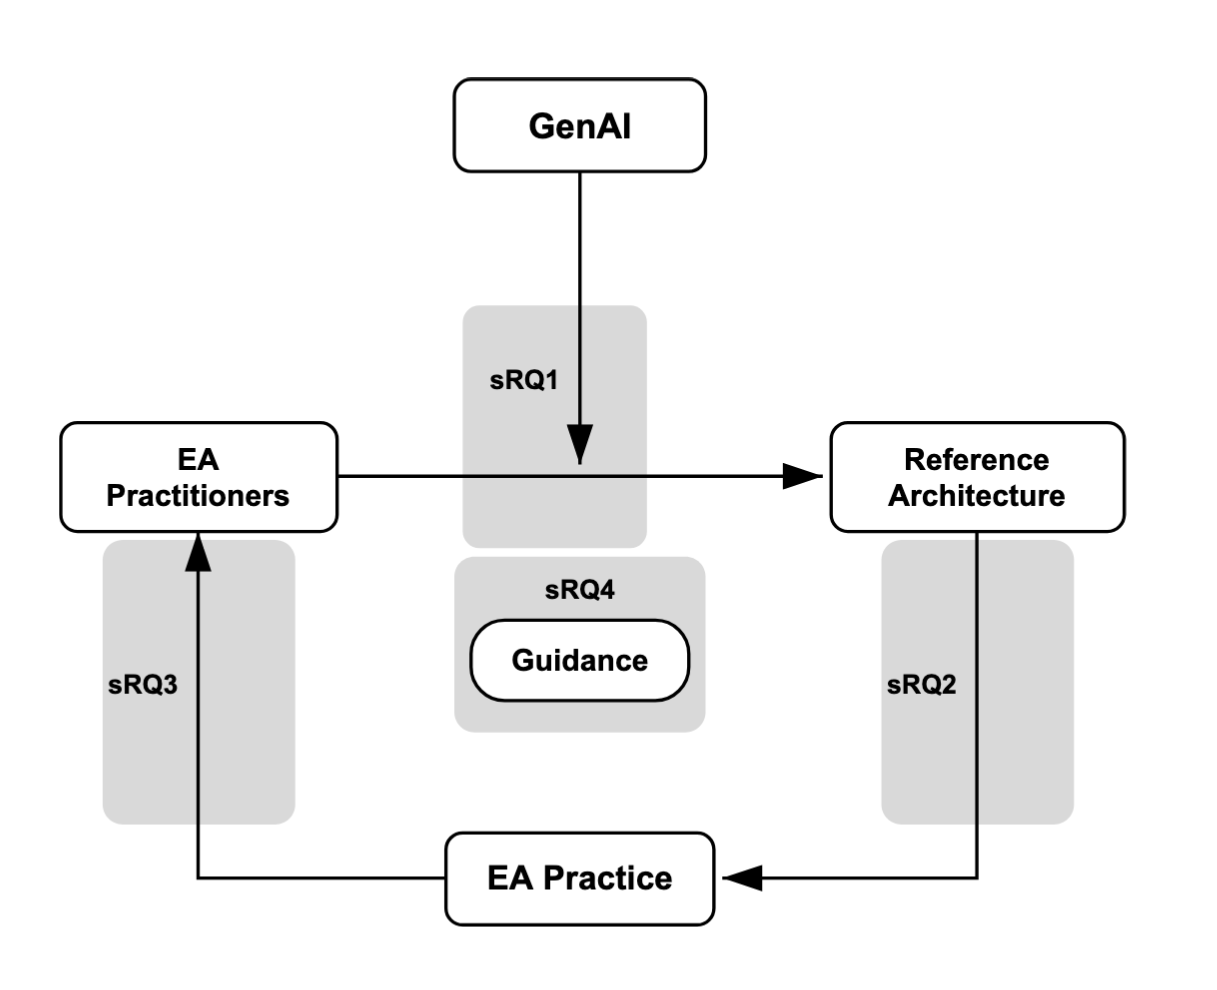
\includegraphics[width=0.7\textwidth]{images/04_1_analyticalFramework.png}
      \caption[Analytical framework for investigating EA-GenAI integration.]{Analytical Framework for Investigating EA-GenAI Integration.}
      \label{fig:analytical-framework}
\end{figure}

Elements and relationships are analysed across individual-collective, descriptive-prescriptive, and temporal dimensions (see Section~\ref{subsec:frameworkdimensions} for tractability within the Delphi design). The five core constructs (GenAI, EA Practitioners, Reference Architecture, EA
Practice, and Guidance) were defined in \textit{Core Constructs for This Study} (Section~\ref{subsec:coreelements}). The
following subsections detail the analytical dimensions and the specific
relationships between these constructs.

\subsubsection{Framework Dimensions}\label{subsec:frameworkdimensions}

Beyond the structural relationships, three analytical dimensions shape how
GenAI integration plays out in practice. Each dimension varies in how directly
the Delphi design can capture it.

\begin{enumerate}
      \item \textbf{Individual-Collective}: Distributed cognition theory
            \parencite{hutchins_cognition_1995} holds that practices develop at both
            individual and collective levels. Practitioners build personal approaches
            while contributing to shared organizational patterns. The Delphi captures
            individual practices through self-report (Round~1) and surfaces collective
            patterns through group deliberation (Rounds~2--3). It does not, however,
            collect organizational-level data; collective dynamics are inferred from
            practitioner accounts.
      \item \textbf{Descriptive-Prescriptive}: The framework separates what is
            happening now (descriptive) from what should happen (prescriptive). The
            descriptive side draws on empirical data from all three rounds. The
            prescriptive side is the researcher's synthesis of that input into a
            guidance artifact, validated through panel consensus (sRQ4) rather than
            field implementation.
      \item \textbf{Temporal}: Practices move from initial experimentation through
            pattern emergence to stabilization. Practitioners and organizations sit at
            different points on this curve. Within the study, temporal dynamics appear
            indirectly: practitioners give retrospective accounts, and the three
            rounds span roughly four months. Longitudinal observation falls outside
            the study's scope but remains an important avenue for future research.
\end{enumerate}

These dimensions are not separate layers; they cut across all elements and
relationships. The Delphi captures the individual-descriptive intersection most
directly, while collective and temporal dynamics are approximated through panel
deliberation and retrospective accounts.

\subsection{Framework Relationships and Manifestations}\label{subsec:framework-relationships}

Each sub-research question examines a specific relationship within the
framework. Understanding each relationship clarifies what the research must
capture and what the methodology must support
(Section~\ref{sec:methodology}).

The subsections below detail each relationship. For sRQ1--sRQ3, the analysis
identifies observable manifestations that inform data collection. For sRQ4, it
addresses how insights from the preceding relationships feed into actionable
guidance. Table~\ref{tab:framework-mapping} summarizes the mapping.

\begin{table}[htbp]
    \centering
    \caption{Mapping of Sub-Questions to Framework Relationships}
    \label{tab:framework-mapping}
    \begin{tabular}{|p{2cm}|p{4cm}|p{3.5cm}|p{4cm}|}
        \hline
        \textbf{Sub-Question} & \textbf{Framework Relationship} & \textbf{Research Focus} & \textbf{Methodological Requirement} \\
        \hline
        sRQ1 & GenAI $\rightarrow$ Reference Architecture (via EA Practitioners) & Current practices & Discovery of emerging patterns \\
        \hline
        sRQ2 & Reference Architecture $\rightarrow$ EA Practice & Practice changes & Capturing evolution effects \\
        \hline
        sRQ3 & EA Practice $\rightarrow$ EA Practitioners & Sense-making & Understanding interpretations \\
        \hline
        sRQ4 & All relationships $\rightarrow$ Guidance & Systematization & Consensus building \\
        \hline
    \end{tabular}
\end{table}

\subsubsection{sRQ1: EA Practitioner-AI Collaboration Patterns}

\textit{"What GenAI practices are EA practitioners currently using when developing RAs?"}
\vspace{0.5em}

This relationship examines how practitioners divide work between themselves and
GenAI when building RAs. Distributed cognition theory
\parencite{hutchins_cognition_1995} frames this as a redistribution of
cognitive labour across human and artificial agents.

Observable manifestations include: which RA activities practitioners delegate to
GenAI versus reserve for human judgment; whether GenAI is consulted continuously
or at specific lifecycle phases; how sophisticated prompt strategies have
become; and which tools or models practitioners prefer for architectural work.

These patterns develop at both individual and collective levels. Individual
experimentation feeds into shared organizational learning, though the pace
varies across practitioners and organizations.

\subsubsection{sRQ2: Artifact-Driven Practice Evolution}

\textit{"What changes to EA practice are EA practitioners experiencing when RAs are developed using GenAI?"}
\vspace{0.5em}

This relationship traces how RAs built with GenAI change broader EA practice.
Because sRQ2 asks what changes practitioners experience, the framework follows
the causal path from GenAI-augmented artifacts back into the practice context.
\textcite{angelov_framework_2012} describe a similar dynamic: reference
architectures influence the application contexts that produced them.

Manifestations include changes in both artifacts and processes. RAs developed
with GenAI may show different structural patterns, documentation styles, or
architectural approaches. Development cycles may speed up or demand new
validation steps. Governance, implementation projects, and knowledge management
practices may all shift as organizations encounter AI-augmented artifacts.

As \textcite{kotusev_enterprise_2018} observed, successful EA practices often
grow bottom-up rather than top-down. GenAI-augmented RAs can accelerate that
kind of organic evolution.

\subsubsection{sRQ3: EA Practitioner Sense-Making and Adaptation}

\textit{"How do EA practitioners make sense of impacts and trade-offs when adopting GenAI for RA development?"}
\vspace{0.5em}

This relationship captures the feedback loop: evolving EA practices shape how
practitioners interpret their situation and decide what to do next.
\textcite{orlikowski_technological_1994}'s concept of technological frames
explains how practitioners update their mental models in response to practice
changes.

Manifestations span cognitive and practical levels. Practitioners develop rules
of thumb for when GenAI adds value versus when it risks compromising
architectural quality. They build validation routines for AI-generated content.
Professional identity shifts as traditional expertise meets new orchestration
skills. Risk awareness grows as practitioners learn the limits of human-AI
collaboration.

This sense-making is collective, not only individual. Interpretations are
shared, debated, and refined within practitioner communities. The resulting
shared understanding shapes how practitioners approach future GenAI
interactions, closing the feedback loop.

\subsubsection{sRQ4: Synthesis into Guidance}

\textit{"How should effective GenAI practices for RA development be systematized into guidance for EA practitioners?"}
\vspace{0.5em}

The fourth sub-question sits at a meta-level: it draws from all three
relationships to produce prescriptive recommendations. From sRQ1, guidance
captures effective collaboration approaches. From sRQ2, it documents quality
criteria and process adaptations. From sRQ3, it incorporates practitioner wisdom
about trade-offs and challenges.

Turning descriptive findings into prescriptive guidance requires assessing
practice maturity, contextual fit, and compatibility with existing EA
frameworks. Because the transformation is researcher-led and validated through
panel consensus, the resulting prescriptions reflect collective judgment rather
than field-tested outcomes.

As \textcite{dellacqua_navigating_2023} observe, AI capability varies
unpredictably across tasks, creating a ``jagged technological frontier.'' The
guidance must accommodate this unevenness. Where practitioner consensus is
strong, directive recommendations are feasible; where it is not, guidance must
remain adaptive. The final artifact form depends on Round~3 findings.

\subsection{Framework Dynamics}\label{subsec:framework-dynamics}

The theoretical review surfaced three reasons why a simple tool-adoption lens
falls short. First, EA work is sociotechnical; it requires negotiation among
diverse stakeholders \parencite{saint-louis_investigation_2019}. Second, GenAI
redistributes cognitive work rather than automating it
\parencite{dellacqua_navigating_2023}. Third, professionals restructure their
practices around AI rather than merely using it as a faster tool
\parencite{noy_experimental_2023}.

These observations point to three dynamics that run through the framework:

\begin{enumerate}
      \item \textbf{Distributed cognition}: the capability of the practitioner-GenAI
            system exceeds what either party contributes alone
            \parencite{hutchins_cognition_1995}. GenAI provides pattern recognition
            across large knowledge spaces; practitioners provide contextual judgment
            and stakeholder awareness.
      \item \textbf{Emergent evolution}: practices arise from situated use
            \parencite{orlikowski_using_2000}, not from technology specifications.
            Initial experiments lead to new RA approaches, which shift practice
            patterns, which update practitioner understanding, which drives further
            experimentation.
      \item \textbf{Multi-level simultaneity}: individual experimentation and
            collective pattern formation happen in parallel. A single practitioner's
            GenAI session is both a personal learning event and a contribution to
            organizational knowledge.
\end{enumerate}

Because the phenomenon keeps evolving, any guidance produced must be designed
for periodic revision as collective understanding matures.

\clearpage
\section{Methodology}\label{sec:methodology}

\subsection*{Introduction}

The conceptual framework (\textit{Conceptual Model}, Section~\ref{sec:conceptual-model}) calls for a
method that can tap distributed expertise, detect new practices as they form,
and produce both analysis and practical guidance. This section describes how a
three-round Design-Oriented Delphi study meets those requirements. Round~1 ran
asynchronously (individual discovery workbooks, January 2026); Rounds~2--3 ran
as synchronous sessions (February--March 2026) using Group Support System (GSS)
technology: software for structured, anonymous group deliberation through
parallel input, voting, and real-time aggregation
\parencite{klein_use_2007, bobbert_group_2013, bobbert_exploring_2017}. The following subsections detail the
research design and implementation:

\localtableofcontents\clearpage

\subsection{Methodological Approach: The Delphi Method}

\subsubsection{Defining the Delphi Method}

The Delphi method is a structured communication technique for enabling
effective group deliberation on complex problems where incomplete knowledge
exists \parencite{linstone_delphi_1975}. The method employs iterative rounds of
data collection and analysis, with controlled feedback between rounds, to
aggregate expert judgment while managing group dynamics
\parencite{dalkey_experimental_1963}.

Classical Delphi characteristics include:

\begin{enumerate}
    \item \textbf{Structured communication}: Information flows through a defined process rather than unstructured discussion.
    \item \textbf{Iteration with feedback}: Multiple rounds allow participants to refine their views based on collective input.
    \item \textbf{Controlled feedback}: Researchers synthesize and present group responses systematically.
    \item \textbf{Expert participation}: Participants are selected based on relevant expertise.
    \item \textbf{Anonymity}: Participants provide input without direct confrontation, reducing dominance effects.
\end{enumerate}

This study incorporates all five characteristics, as detailed in the research
design below.

\subsubsection{Justification for an Exploratory-Convergent Design}

GenAI integration in EA practice is new enough that imposing predetermined
categories would miss novel practices
\parencite{okoli_delphi_2004}. The research therefore begins with open
discovery before moving to structured convergence
\parencite{schmidt_managing_1997}. Synchronous rounds then compress the
timeline while maintaining iterative refinement, and combining asynchronous
depth with synchronous interaction draws on the strengths of both modes
\parencite{gordon_rt_2006}.

\subsection{Research Design: Exploratory-Convergent Design-Oriented Synchronous Delphi}

\subsubsection{Positioning Within Delphi Typology}

The study combines three Delphi orientations. Exploratory Delphi enables
open-ended discovery of undocumented practices
\parencite{okoli_delphi_2004}. Convergent Delphi provides mechanisms for
progressive synthesis toward consensus \parencite{linstone_delphi_1975}.
Design Delphi focuses on producing actionable artifacts
\parencite{skulmoski_delphi_2007}. \textcite{day_generic_2005} argue that
Delphi designs should be tailored to research purposes rather than following a
single typology; this study does so by sequencing exploration, convergence, and
design so that each phase builds on the outputs of the previous one. Each
component follows established Delphi principles (iteration, controlled
feedback, expert participation), and documented protocols for every phase
support replication.

\subsubsection{The Emergent Artifact Approach}\label{subsec:design-choices}

Building on Delphi scholarship that emphasizes responsiveness to participant
input \parencite{linstone_delphi_1975}, this study adopts a practitioner-grounded
emergence approach. The guidance artifact develops progressively from
practitioner data rather than being presented as a preliminary instrument in any
round.
Specifically:

\begin{enumerate}
    \item \textbf{Round~1: No artifact presented}: practitioners document their
          discovered practices
    \item \textbf{Between Rounds~1--2}: researcher synthesizes practices into
          initial patterns
    \item \textbf{Round~2}: emergent patterns presented for validation
    \item \textbf{Between Rounds~2--3}: researcher refines artifact based on
          validation data
    \item \textbf{Round~3}: practitioners critique a refined draft artifact and
          provide input for remaining gaps
    \item \textbf{Post-Round~3}: researcher finalizes guidance artifact
\end{enumerate}

As illustrated in Figure~\ref{fig:emergent-artifact}, the guidance artifact
evolves through iterative rounds, beginning with practitioner-generated data
and progressively refined through researcher synthesis and collective
validation.

\begin{figure}[H]
    \centering
    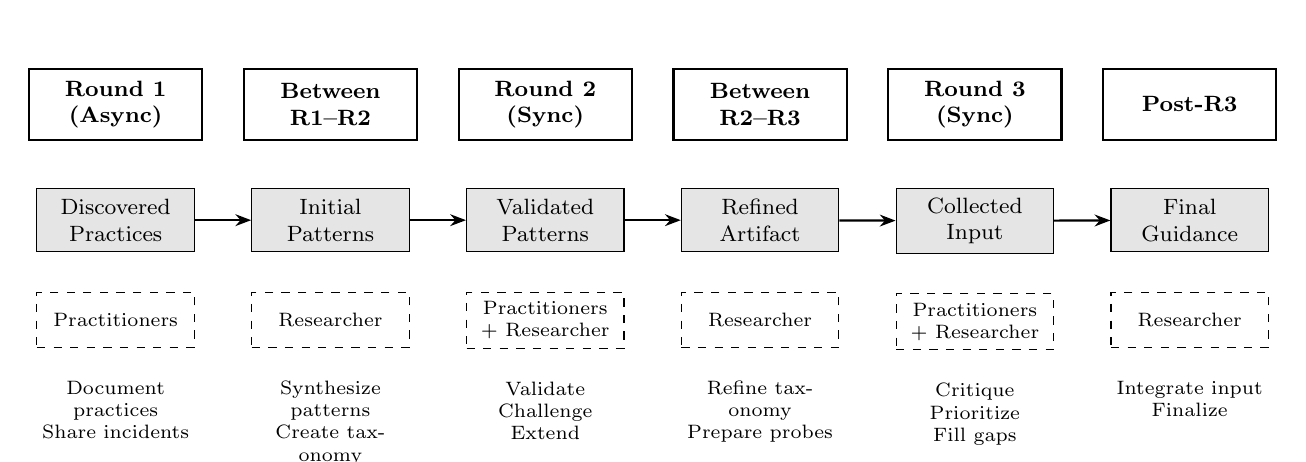
\begin{tikzpicture}[
        node distance=0.6cm and 0.5cm,
        phase/.style={rectangle, draw=black, thick, minimum width=2.2cm, minimum height=0.9cm, align=center, font=\footnotesize\bfseries},
        artifact/.style={rectangle, draw=black, fill=gray!20, minimum width=2.0cm, minimum height=0.8cm, align=center, font=\footnotesize},
        actor/.style={rectangle, draw=black, dashed, minimum width=2.0cm, minimum height=0.7cm, align=center, font=\scriptsize},
        activity/.style={align=center, font=\scriptsize, text width=2.0cm},
        arrow/.style={-{Stealth[length=2mm]}, thick},
        ]

        % Phase headers (top row)
        \node[phase] (r1) {Round 1\\(Async)};
        \node[phase, right=of r1] (between12) {Between\\R1--R2};
        \node[phase, right=of between12] (r2) {Round 2\\(Sync)};
        \node[phase, right=of r2] (between23) {Between\\R2--R3};
        \node[phase, right=of between23] (r3) {Round 3\\(Sync)};
        \node[phase, right=of r3] (post) {Post-R3};

        % Artifact boxes (middle row)
        \node[artifact, below=of r1] (a1) {Discovered\\Practices};
        \node[artifact, below=of between12] (a2) {Initial\\Patterns};
        \node[artifact, below=of r2] (a3) {Validated\\Patterns};
        \node[artifact, below=of between23] (a4) {Refined\\Artifact};
        \node[artifact, below=of r3] (a5) {Collected\\Input};
        \node[artifact, below=of post] (a6) {Final\\Guidance};

        % Arrows between artifacts
        \draw[arrow] (a1) -- (a2);
        \draw[arrow] (a2) -- (a3);
        \draw[arrow] (a3) -- (a4);
        \draw[arrow] (a4) -- (a5);
        \draw[arrow] (a5) -- (a6);

        % Actor boxes (third row)
        \node[actor, below=0.5cm of a1] (act1) {Practitioners};
        \node[actor, below=0.5cm of a2] (act2) {Researcher};
        \node[actor, below=0.5cm of a3] (act3) {Practitioners\\+ Researcher};
        \node[actor, below=0.5cm of a4] (act4) {Researcher};
        \node[actor, below=0.5cm of a5] (act5) {Practitioners\\+ Researcher};
        \node[actor, below=0.5cm of a6] (act6) {Researcher};

        % Activities (bottom row)
        \node[activity, below=0.3cm of act1] (actv1) {Document practices\\Share incidents};
        \node[activity, below=0.3cm of act2] (actv2) {Synthesize patterns\\Create taxonomy};
        \node[activity, below=0.3cm of act3] (actv3) {Validate\\Challenge\\Extend};
        \node[activity, below=0.3cm of act4] (actv4) {Refine taxonomy\\Prepare probes};
        \node[activity, below=0.3cm of act5] (actv5) {Critique\\Prioritize\\Fill gaps};
        \node[activity, below=0.3cm of act6] (actv6) {Integrate input\\Finalize};


    \end{tikzpicture}
    \caption[Emergent artifact development process across six phases.]{Emergent Artifact Development Process.}\label{fig:emergent-artifact}
\end{figure}

The guidance artifact evolves through six phases: practitioner discovery (Round~1), researcher synthesis (between rounds), collective validation (Round~2), researcher refinement (between rounds), practitioner critique (Round~3), and researcher finalization (post-Round~3). This approach aligns with grounded theory principles
\parencite{charmaz_constructing_2014} where categories emerge from data rather
than being predetermined.

\subsubsection{Exploration and Development}

The three rounds pursue sequential objectives. Round~1 focused on discovery:
uncovering practices without researcher bias. Round~2 shifted toward
convergence, validating patterns and identifying commonalities across
practitioner experiences. Round~3 emphasized development, synthesizing
collective expertise into practical guidance. This progression keeps
prescriptive outputs grounded in descriptive findings.

\subsection{Literature Review}\label{subsec:literature-review}

This subsection describes how the theoretical foundation
(Section~\ref{sec:theoretical-background}) was built. The literature review
followed a diverge-converge process
\parencite{botjes_antifragile_2020} that moved from broad exploration to
focused selection, with the researcher's prior interests shaping the initial
search direction.

The research began with a practical question: how does Generative AI (GenAI)
impact team cognitive load for Enterprise Architecture (EA) practitioners? The
researcher's background as a Team Topologies Advocate
\parencite{skelton_team_topologies_2019} provided an initial lens.
\textcite{skelton_team_topologies_2019} adapted Cognitive Load Theory
\parencite{sweller_cognitive_1988} to software delivery teams, arguing that team
cognitive load determines delivery effectiveness. However, tracing this
adaptation back to \textcite{sweller_cognitive_1988}'s original Cognitive Load
Theory revealed that the extrapolation from individual cognition to team-level
load was more a conceptual stretch than a direct theoretical extension.

This gap led to \textcite{hutchins_cognition_1995}'s distributed cognition,
which treats cognitive processes as distributed across people, artifacts, and
environments rather than confined to individual minds. Distributed cognition
proved a better theoretical fit, because it accounts for how cognitive work
redistributes across human and artificial agents without requiring the
individual-to-team extrapolation that Cognitive Load Theory demands. At the same
time, EA practice proved too broad a scope. The rapid growth of GenAI coding
tools was already reshaping software architecture and design
\parencite{peng_impact_2023}, so the researcher narrowed the focus to one
specific task: the Reference Architecture (RA) lifecycle, encompassing creating,
updating, consuming, and learning from RAs. This combination of distributed
cognition as theoretical lens and RA development as empirical scope shaped the
theoretical foundation (Section~\ref{sec:theoretical-background}).

\subsubsection{Diverge-Converge Process}

The literature search followed a diverge-converge process, adapted from
\textcite{botjes_antifragile_2020}. As illustrated in
Figure~\ref{fig:diverge-converge}, the divergence phase creates choices by
exploring broadly from primary sources outward to secondary and tertiary
sources. The convergence phase makes choices by filtering sources through
categories and keywords to determine relevance and scope.

\begin{figure}[htbp]
    \centering
    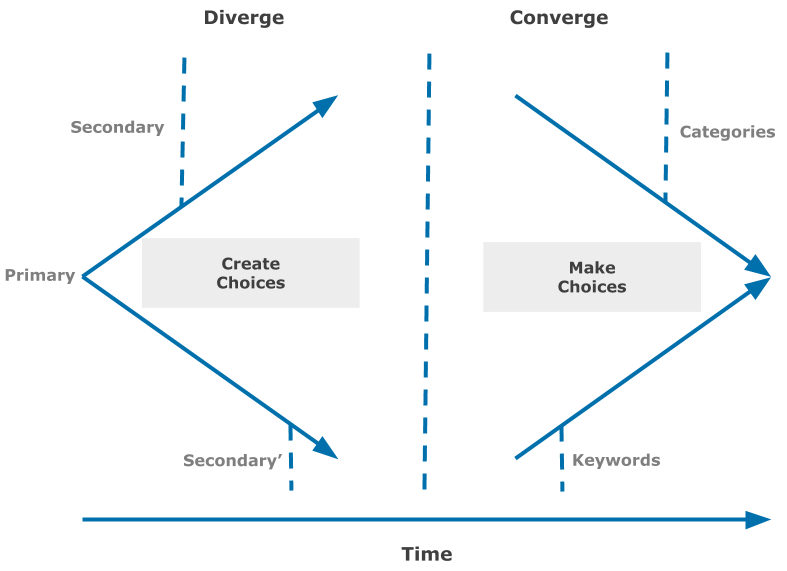
\includegraphics[width=0.75\textwidth]{images/diverge-converge.png}
    \caption[Diverge and Converge process for literature review.]{Diverge and
    Converge process. The divergence phase expands the search space from primary
    sources outward; the convergence phase filters by categories and keywords.
    Source: \textcite{botjes_antifragile_2020}.}\label{fig:diverge-converge}
\end{figure}

Both phases were iterative. New sources discovered during convergence sometimes
triggered additional divergence cycles as citation trails revealed unexpected
connections. The path from Team Topologies
\parencite{skelton_team_topologies_2019} to Cognitive Load Theory
\parencite{sweller_cognitive_1988} to distributed cognition
\parencite{hutchins_cognition_1995} exemplifies this iterative process: each
discovery opened new search directions before convergence narrowed the focus.

\subsubsection{Search Strategies}

Three complementary strategies populated the diverge-converge process.

\textbf{Systematic database search.} An EBSCO host search (June 2025) targeted
top Information Systems journals using combinations of ``enterprise
architecture,'' ``reference architecture,'' ``generative AI,'' and ``large
language models''\footnote{EBSCO host advanced search conducted on June 8, 2025,
    resulted in 0 publications using the query: ((enterprise architecture OR ea
    practice) AND (gen ai OR generative artificial intelligence OR llm OR large
    language models)) AND SO (MIS Quarterly Executive OR Information Systems
    Research OR Journal of the Association for Information Systems OR European
    Journal of Information Systems). Filters applied: peer-reviewed articles,
    publication date from January 1, 2020, to June 8, 2025.}.
The near-zero results confirmed the research gap that motivates this study.

\textbf{Backward and forward citation tracing.} Foundational works served as
primary sources for snowball searches. Starting from
\textcite{zachman_zachman_1987} and \textcite{kotusev_enterprise_2018} for
Enterprise Architecture (EA), \textcite{hutchins_cognition_1995} and
\textcite{hollan_distributed_2000} for distributed cognition,
\textcite{skelton_team_topologies_2019} and
\textcite{sweller_cognitive_1988} for Cognitive Load Theory, and
\textcite{angelov_framework_2012} and \textcite{cloutier_concept_2010} for
Reference Architectures, citation tracing identified additional sources across
these domains. This strategy proved the most productive, yielding the majority
of the theoretical foundation's sources.

\textbf{Practitioner and grey literature.} Industry reports from the
International Energy Agency \parencite{iea_energy_2025}, McKinsey
\parencite{mckinsey_cost_2025}, Microsoft \parencite{microsoft_wti_2025}, and
Stack Overflow developer surveys \parencite{stack_overflow_2024,
stack_overflow_2025} provided empirical context for GenAI adoption trends and
infrastructure investment data not yet covered in peer-reviewed outlets.

Source selection prioritized peer-reviewed publications. Grey literature was
used only for adoption statistics and infrastructure data. The resulting
theoretical foundation (Section~\ref{sec:theoretical-background}) synthesizes
these sources into the five constructs and integrating lens that inform the
conceptual model (Section~\ref{sec:conceptual-model}).

\subsection{Research Implementation}

This subsection describes the expert panel selection, the hybrid round
structure, data collection and analysis procedures, and detailed round
protocols.

\subsubsection{Expert Panel Selection}\label{subsec:expert-panel}

The expert panel was designed for 8--12 EA practitioners selected through
purposive sampling \parencite{patton_qualitative_2015}. Eight participated in
Round~1, ten of twelve invited joined Round~2, and seven of ten invited
attended Round~3. Inclusion required current
hands-on experience using GenAI in EA practice for at least six months and
minimum five years as an EA practitioner to ensure foundational expertise.
Candidates also needed active involvement in Reference Architecture
development and willingness to participate across rounds. Consistent with
\textcite{kotusev_enterprise_2018}'s finding that architectural artifacts involve
distributed authorship, the panel deliberately includes professionals beyond the
``enterprise architect'' title. Participants hold roles including enterprise
architect, solution architect, platform engineer, enterprise data architect,
software architect, and freelance architectural consultant. This role diversity
reflects how RA development unfolds in practice across organizational
boundaries.

For Round~2, the panel was deliberately expanded from the original eight
participants to twelve invitees (five returning from Round~1, seven new).
This expansion served a methodological purpose: pattern validation benefits
from perspectives not anchored to the respondents' own Round~1 submissions,
reducing confirmation bias in category assessment. All new participants met
the same inclusion criteria. Ten of twelve attended. For Round~3, all seven
participants were returning from earlier rounds, ensuring continuity during
the final convergence phase.

The panel composition seeks diversity across four dimensions: industry sectors
(financial services, retail, technology, government), organizational size (SME
to Fortune 500), geographic distribution within European timezone constraints,
and varying levels of GenAI integration depth.
This sample size aligns with \textcite{skulmoski_delphi_2007}, who suggest
that 8--12 experts provide sufficient diversity while enabling meaningful
synchronous interaction. This sampling strategy prioritises information richness
and expert insight over statistical representativeness
\parencite{patton_qualitative_2015}; the resulting panel captures frontier
practice among active GenAI adopters rather than the breadth of the EA
practitioner population.

\subsubsection{Hybrid Delphi Round Structure}

The study combines asynchronous and synchronous elements, moving from
individual discovery to collective sensemaking.
Figure~\ref{fig:delphi-process} shows the complete process flow across all
three rounds.

\begin{figure}[!ht]
    \centering
    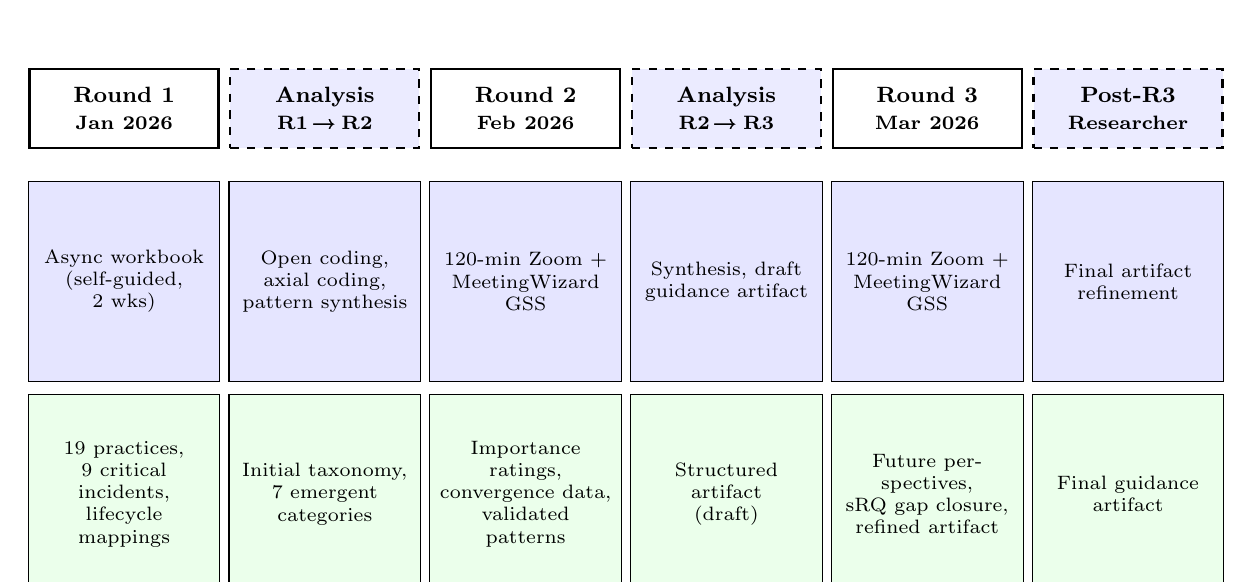
\begin{tikzpicture}[
        % Round nodes: solid border, white fill
        round/.style={rectangle, draw=black, thick, fill=white,
            minimum width=2.4cm, minimum height=1.0cm,
            align=center, font=\footnotesize\bfseries},
        % Analysis nodes: dashed border, light fill
        analysis/.style={rectangle, draw=black, thick, dashed, fill=blue!8,
            minimum width=2.4cm, minimum height=1.0cm,
            align=center, font=\footnotesize\bfseries},
        % Detail and output boxes use a fixed-size \vbox so ALL boxes are
        % exactly the same height regardless of content (5 lines max).
        detail/.style={rectangle, draw=black, fill=blue!10,
            minimum width=2.4cm,
            font=\scriptsize, text width=2.2cm, align=center,
            execute at begin node={\vbox to 2.3cm\bgroup\vfil},
            execute at end node={\vfil\egroup}},
        output/.style={rectangle, draw=black, fill=green!8,
            minimum width=2.4cm,
            font=\scriptsize, text width=2.2cm, align=center,
            execute at begin node={\vbox to 2.3cm\bgroup\vfil},
            execute at end node={\vfil\egroup}},
        ]

        % Column x-coordinates (evenly spaced to fit within \textwidth)
        \def\colsep{2.55cm}
        % Row y-coordinates (spacing for 6-line boxes)
        \def\rowB{-2.2}
        \def\rowC{-4.9}

        % === Top row: phase headers ===
        \node[round] (r1) at (0,0) {Round~1\\{\scriptsize Jan 2026}};
        \node[analysis] (a12) at (\colsep,0) {Analysis\\{\scriptsize R1\,\textrightarrow\,R2}};
        \node[round] (r2) at (2*\colsep,0) {Round~2\\{\scriptsize Feb 2026}};
        \node[analysis] (a23) at (3*\colsep,0) {Analysis\\{\scriptsize R2\,\textrightarrow\,R3}};
        \node[round] (r3) at (4*\colsep,0) {Round~3\\{\scriptsize Mar 2026}};
        \node[analysis] (post) at (5*\colsep,0) {Post-R3\\{\scriptsize Researcher}};

        % === Middle row: method / format ===
        \node[detail] (d1) at (0,\rowB) {Async workbook\\(self-guided, 2 wks)};
        \node[detail] (d12) at (\colsep,\rowB) {Open coding,\\axial coding,\\pattern synthesis};
        \node[detail] (d2) at (2*\colsep,\rowB) {120-min Zoom +\\MeetingWizard GSS};
        \node[detail] (d23) at (3*\colsep,\rowB) {Synthesis, draft\\guidance artifact};
        \node[detail] (d3) at (4*\colsep,\rowB) {120-min Zoom +\\MeetingWizard GSS};
        \node[detail] (dpost) at (5*\colsep,\rowB) {Final artifact\\refinement};

        % === Bottom row: key outputs ===
        \node[output] (o1) at (0,\rowC) {19 practices,\\9 critical incidents,\\lifecycle mappings};
        \node[output] (o12) at (\colsep,\rowC) {Initial taxonomy,\\7 emergent\\categories};
        \node[output] (o2) at (2*\colsep,\rowC) {Importance ratings,\\convergence data,\\validated patterns};
        \node[output] (o23) at (3*\colsep,\rowC) {Structured artifact\\(draft)};
        \node[output] (o3) at (4*\colsep,\rowC) {Future perspectives,\\sRQ gap closure,\\refined artifact};
        \node[output] (opost) at (5*\colsep,\rowC) {Final guidance\\artifact};

    \end{tikzpicture}
    \caption[Delphi process flow with data progression across three rounds.]{Delphi process flow with data progression. Three expert rounds (solid borders) alternate with researcher analysis phases (dashed borders). The middle row (blue) shows the method used in each phase; the bottom row (green) shows the key outputs.}\label{fig:delphi-process}
\end{figure}

\textbf{Round~1 (Asynchronous, January 2026)}: Individual exploration over two weeks

\begin{enumerate}
    \item Participants received a discovery workbook via email
    \item Completed structured sections at their own pace
    \item Documented GenAI practices with rich contextual detail
    \item Provided narrative accounts of critical incidents
    \item Rated confidence and maturity of their practices
\end{enumerate}

\textbf{Rounds~2--3 (Synchronous, February--March 2026)}: Collective refinement

\begin{enumerate}
    \item 120-minute online sessions using Zoom\footnote{Zoom Video Communications: \url{https://zoom.us/}} for video conferencing and MeetingWizard\footnote{MeetingWizard is a cloud-based Group Support System (GSS) platform that structures sessions through agenda creation, anonymous brainstorming, structured voting, and real-time result aggregation, automatically generating reports that capture all discussions and outcomes. See \url{https://www.meetingwizard.nl/en/}} for group deliberation
    \item Real-time validation and exploration of emergent patterns
    \item Dynamic consensus building with technological support
    \item Progressive refinement of guidance artifact
\end{enumerate}

\subsubsection{Data Collection and Analysis}

Each round yields progressively more structured data.

In the asynchronous Round~1, participants describe two to five discovered
practices with step-by-step narratives and genesis stories. They map each
practice to RA lifecycle phases and share three to five critical incidents
(success and failure stories with supporting evidence). They also complete
impact assessments covering time, quality, and role changes; document
challenges and workarounds; and contribute emergent wisdom, including
counterintuitive discoveries and predictions about future practice evolution.

The synchronous Rounds~2--3 generated convergence data through structured GSS
activities. Participants rated the importance of emergent practice categories
on five-point scales and contributed to brainstorms on lifecycle mapping,
practice changes, and trust calibration. Facilitated flipboard discussions
explored boundary conditions and cross-role dynamics. Priority voting
established collective importance weighting, while open-ended brainstorm
responses captured why specific practices work or fail in particular contexts.
Throughout these rounds, participants contributed refinements to the emerging
guidance artifact.

\subsubsection{Round Protocols}

This subsection details the protocol for each round: Round~1 (asynchronous
discovery), Round~2 (synchronous validation), and Round~3 (synchronous final
refinement).

\textbf{Round~1: Asynchronous Exploration (January 2026)}

\textbf{Objective}: Open discovery of emerging practices without researcher framing

\paragraph{Two-Week Structure}

Round~1 gives participants two weeks to complete a discovery workbook at their
own pace. No preliminary artifact or taxonomy is presented; the workbook uses
sensitizing prompts that guide exploration without suggesting predetermined
categories. Guided prompts ensure comparable data across participants, while
free-text responses let practitioners describe practices in their own terms.
Table~\ref{tab:r1-timeline} shows the timeline.

\begin{table}[h]
    \centering
    \caption{Round~1 Timeline and Activities}
    \label{tab:r1-timeline}
    \begin{tabular}{|p{2cm}|p{4cm}|p{4cm}|p{4cm}|}
        \hline
        \textbf{Day}                                                    & \textbf{Activity}       & \textbf{Deliverable}                    & \textbf{Expected Output}           \\
        \hline
        Day 1                                                           & Launch exploration      &
        \begin{itemize}[leftmargin=*,topsep=0pt,itemsep=0pt]
            \item Problem context document
            \item Discovery workbook
            \item Standard RA lifecycle
        \end{itemize} & Participant orientation                                                                                                           \\
        \hline
        Days 2--10                                                       & Self-guided discovery   & Participants complete workbook sections & 2--5 core practices per participant \\
        \hline
        Day 11--12                                                       & Reflection prompts      & Additional prompts for unexplored areas & Completeness check                 \\
        \hline
        Day 13--14                                                       & Submission deadline     & Completed workbooks                     & \textasciitilde19 total practices  \\
        \hline
        Days 15--25                                                      & Intensive analysis      & Pattern emergence and synthesis         & Initial taxonomy and guidance \\
        \hline
    \end{tabular}
\end{table}

\paragraph{Discovery Workbook Design}

The discovery workbook serves as the primary data collection instrument,
structured to guide systematic exploration while avoiding constraining
participants' responses. The workbook employs a progressive structure that
moves from context setting through practice discovery to reflective
sensemaking.

We deliberately framed the workbook scope as ``Software Architecture / Solution
Design work'' rather than ``Enterprise Architecture.'' This choice reflects a
terminological broadening, not a scope expansion. Practitioners who create,
update, and govern Reference Architectures often describe this work as
``solution design'' or ``software architecture'' rather than ``RA development.''
A strict EA framing risked excluding professionals who materially shape
architectural artifacts but do not identify as enterprise architects: solution
architects, platform engineers, and senior developers whose daily work involves
Reference Architectures
\parencite[see Section~\ref{sec:theoretical-background}]{kotusev_enterprise_2018}.

This terminological broadening introduces a validity tension. Practices
discovered under a ``Software Architecture'' framing may extend beyond
RA-specific work into general architectural practice, blurring the boundary
with the research question's ``EA practitioners'' scope. Two instrument design
features mitigate this risk. First, Part~C of the workbook requires
participants to map each practice to eight RA lifecycle phases, structurally
anchoring reported practices to RA development regardless of the terminology
used to invite participation. Second, the R2 validation session evaluated
practices specifically in the context of RA development: ten participants from
diverse architectural roles all recognized their practice in the workbook
prompts. By meeting practitioners in their own terminology while anchoring
responses to the RA lifecycle, the instrument captured practices that a narrower
EA-only framing might have excluded without sacrificing scope specificity.

The workbook comprises seven parts. Part~A establishes the
participant's GenAI tooling, experience level, and organizational context.
Part~B (Practice Archaeology) forms the core discovery section, prompting
participants to recall genesis moments and systematically document each named
practice with its problem, step-by-step process, effectiveness rate, and
failure modes. Part~C asks participants to map their practices to eight RA
lifecycle phases and identify tasks that must remain human-performed. Part~D
solicits three to five critical incident narratives with structured fields for
context, action, result, insight, and supporting evidence. Part~E captures
impact reflections across three dimensions: time and effort, quality and
completeness, and role evolution. Part~F documents challenges encountered along
with workarounds and capability wishes. Part~G elicits emergent wisdom,
including advice for colleagues, counterintuitive discoveries, and twelve-month
predictions. This structure balances guided prompts for cross-participant
comparability with free-text responses that allow practitioners to describe
practices in their own terms. The complete workbook instrument is provided in
\ref{app:workbook}.

\paragraph{Data Collection Platform}

The workbook was deployed as a structured Word document distributed via email,
providing:
\begin{itemize}
    \item Completion over multiple sessions at the participant's own pace
    \item Structured sections guiding progressive exploration
    \item Rich text formatting for detailed descriptions
    \item Clear section delineation to encourage completeness
\end{itemize}

\paragraph{Outputs}

Round~1 yielded:
\begin{itemize}
    \item 19 distinct practice descriptions (\textasciitilde2--3 per participant $\times$ 8 participants)
    \item 9 critical incident narratives with evidence
    \item Practice-to-lifecycle mappings across all workbook sections
    \item 12 challenges with workarounds
    \item 8 sets of emergent wisdom and predictions
\end{itemize}

This dataset underwent intensive analysis (Days 15--25) to identify emergent
patterns, create an initial practice taxonomy, and develop the first version of
the guidance artifact for validation in Round~2.

\textbf{Round~2: Synchronous Pattern Validation (4 February 2026)}

\textbf{Objective}: Validate emergent patterns from Round~1 and explore variations

Round~2 was conducted as a 120-minute synchronous session via Zoom\footnote{\url{https://zoom.us/}} with
MeetingWizard\footnote{\url{https://www.meetingwizard.nl/en/}} GSS technology \parencite[see also][for a recent application in EA research]{nieuwenhuis_towards_2025}. Ten of twelve invited participants joined. The
session presented emergent practice categories synthesized from Round~1
analysis for collective validation. The planned 15-step protocol was partially
executed during the synchronous session: Steps~1--7 (opening, practice
presentation, brainstorm on reactions and gaps, flipboard discussion on
practice categories, importance voting, lifecycle mapping brainstorm, and
before/after brainstorm) were completed in real time. Two remaining voting
steps (Change Significance and Heuristic Agreement) were collected
asynchronously afterward; all ten participants completed these votes. The
session generated convergence data on practitioner agreement levels and
cross-cutting patterns, providing input for the evolving guidance artifact.

\textbf{Round~3: Synchronous Final Refinement (4 March 2026)}

\textbf{Objective}: Gather future-oriented data, address remaining sub-research-question gaps, and collect input for the final guidance artifact

Round~3 was the final synchronous session, building on the validated practice
categories from Round~2. Seven of ten invited participants attended the
120-minute session; all seven were returning participants from earlier rounds.
The session was designed around three objectives. First, it aimed to elicit
forward-looking perspectives on how GenAI practices in RA development may
evolve. Second, it collected data for sub-research-questions not yet fully
addressed, particularly sRQ3 on sensemaking and sRQ4 on systematization.
Third, it gathered practitioner input to refine the draft guidance artifact.
Procedural deviations from the planned 16-step protocol are documented in
Section~\ref{subsec:data-limitations}.

Preliminary analysis of Rounds~1 and~2 had surfaced cross-role dynamics as an
emergent theme. \textcite{kotusev_enterprise_2018}'s finding that architectural
artifacts involve distributed authorship provided theoretical grounding for
this observation. This motivated three targeted R3 probes: how developer-level
GenAI use informs architectural artifacts bottom-up, what traceability
mechanisms practitioners employ when GenAI distributes authorship across roles,
and where governance friction arises when non-architects produce architectural
outputs.

\subsection{Data Analysis Framework}

The hybrid design requires distinct analytical approaches for the discovery
phase versus the convergence phases:

\subsubsection{Round~1 Discovery Analysis (Days 15--25)}

The discovery analysis proceeds through four phases over Days 15--25.
Phase~1 (data immersion) involves reading all workbooks, memoing first
impressions, and creating participant profiles. Phase~2 (open coding) fractures
data into discrete concepts using line-by-line, in-vivo, incident, process,
and emotion coding \parencite{charmaz_constructing_2014}. Phase~3 (pattern
emergence) applies axial coding: identifying relationships between practices,
comparing across participants, and clustering similar practices into
preliminary categories.

These coding phases produced four coding dimensions that
structure the Round~1 findings reported in Section~\ref{sec:results}:
\emph{interaction patterns} (how practitioners engage GenAI, from research
assistant to deep integration), \emph{distribution of cognitive tasks} (which
tasks practitioners delegate versus retain), \emph{engagement quality} (the
degree of active oversight practitioners maintain over GenAI outputs), and
\emph{practice reconfiguration} (how established workflows changed with GenAI
adoption). These dimensions emerged abductively: initial codes were derived
inductively from practitioner language, then organized through constant
comparison against the distributed cognition lens established in
Section~\ref{sec:conceptual-model}
\parencite{charmaz_constructing_2014, patton_qualitative_2015}. Together, the
four dimensions provided a consistent analytical vocabulary for coding all 19
discovered practices and the cross-cutting patterns across the panel.

Phase~4 (synthesis) creates a practice taxonomy, maps practices to RA
lifecycle phases, documents variation patterns, and prepares validation
materials for Round~2. Three analytical decisions guide the process:
practitioner language is preserved in category names, minority practices are
kept even when mentioned by few participants, and contradictions are documented
as variation points rather than treated as errors.

In addition to these coding categories, cross-role dynamics serve as an
emergent analytical dimension. Round~1 revealed that practitioners routinely
described practices crossing traditional role boundaries; what the coded
analysis labels Pattern~4. Round~2's panel diversity reinforced this
observation: inside-out workflows and collective decision capture surfaced
precisely because participants held varied architectural roles. This dimension
complements the existing coding categories (in-vivo, incident, process,
emotion) as a thematic lens for identifying how GenAI redistributes
architectural work across organizational roles.
\textcite{hollan_distributed_2000}'s distributed cognition framework (where
cognitive processes distribute across individuals, artifacts, and
environments) grounds this analytical choice theoretically.

\subsubsection{Between-Round Analysis (Synchronous Rounds)}

\paragraph{Round~2 $\rightarrow$ 3 Analysis}
\begin{itemize}
    \item Synthesized Round~2 importance ratings and variability profiles per
          practice category
    \item Confirmed seven practice categories; no category revisions required
    \item Prepared structured artifact with six elements per practice
          (description, lifecycle phases, guidance level, experience indicators,
          verification patterns, cross-role considerations)
    \item Designed targeted Round~3 probes based on emergent gaps (cross-role
          dynamics, trust calibration)
\end{itemize}

\paragraph{Round~3 Final Analysis}
\begin{itemize}
    \item Calculated consensus and variability metrics for all Round~3 voting
          items (heuristics, cross-role patterns, guidance priorities)
    \item Organized verification heuristics into tiers based on consensus strength
    \item Analyzed cross-role pattern significance; noted high variability as
          context-dependent rather than universal
    \item Integrated guidance element priority ratings into final artifact
          structure
    \item Finalized guidance artifact incorporating all three rounds of data
\end{itemize}

\subsection{Quality Criteria}

This subsection addresses methodological rigor, trustworthiness, and the
study's limitations and delimitations.

\subsubsection{Rigor in Exploratory-Convergent Delphi}

Discovery validity in Round~1 is established through open-ended exploration
where no researcher-imposed categories constrain what participants can report.
Rich description through detailed narratives enables thick interpretation of
practitioner experiences. Evidence grounding ensures that actual prompts and
outputs support practitioner claims. Negative case analysis explicitly solicits
failures and challenges alongside successes.

Convergence validity in Rounds~2--3 relies on four mechanisms. Member checking
ensures participants validate interpretations at each round. Consensus metrics
provide transparent reporting of agreement levels. Variation documentation
preserves divergence without forcing artificial agreement, and progressive
refinement enables iterative improvement across multiple rounds.

\subsubsection{Trustworthiness Criteria}

Delphi studies face established methodological critiques, particularly
concerning researcher influence during synthesis, pressure toward artificial
consensus, and arbitrary definitions of expertise
\parencite{linstone_delphi_1975, okoli_delphi_2004}. Following
\textcite{lincoln_naturalistic_1985}, this research addresses these risks
through four trustworthiness criteria.

\textbf{Credibility} addresses the risk of researcher bias in interpreting and
synthesizing participant responses. This study establishes credibility through
prolonged engagement across three rounds over four months, allowing the researcher
to develop deep familiarity with practitioner perspectives. Triangulation across
multiple data types (narratives, ratings, and group discussions) reduces
dependence on any single source. Member checking at each round ensures
participants validate researcher interpretations before subsequent rounds build
upon them. The analysis explicitly seeks negative cases, including failures and
divergent views, rather than selecting only confirmatory evidence. Regular peer
debriefing with the research supervisor provides external challenge to emerging
interpretations.

\textbf{Transferability} addresses the risk that arbitrary or unclear expert
selection limits the applicability of findings to broader contexts. The research
provides thick description of participant organizational contexts, enabling
readers to assess relevance to their own situations. Boundary conditions for
guidance applicability are specified explicitly, acknowledging where practices transfer and where they do not. Documentation of practice variations across contexts
preserves important distinctions rather than forcing premature generalization.
The clear articulation of participant selection criteria in
Section~\ref{sec:methodology} allows readers to evaluate the expertise base
underlying the findings.

\textbf{Dependability} addresses the risk of subjective analytical decisions
lacking transparency. A comprehensive audit trail documents all analytical
decisions, from initial coding through pattern synthesis to final guidance
formulation. Code-recode reliability checks at two-week intervals ensure
consistency in the researcher's interpretive framework over time. External
advisor review of the coding framework provides independent validation of
analytical categories. Version control for the guidance artifact (tracking its
evolution across rounds) makes visible how collective input shaped the
final output.

\textbf{Confirmability} addresses the risk that controlled feedback creates
pressure toward artificial consensus, suppressing minority views. Reflexive notes captured at key analytical decision points document the
researcher's evolving assumptions and their potential influence on
interpretation. Direct
participant quotes support all substantive interpretations, grounding claims in
participant voice rather than researcher inference. Divergent views are
explicitly preserved in the final guidance rather than eliminated in pursuit of
false unanimity. Raw data remains available for audit, enabling independent
verification of the analytical process.

\subsubsection{Limitations}

The methodology faces both methodological and scope limitations.
Methodologically, discovery is limited to current practitioners, missing the
perspective of non-adopters who tried and rejected GenAI integration.
Practices are self-reported without direct observation, introducing recall
bias. Social desirability bias likely persists despite anonymity measures.
The synthesis between rounds requires researcher interpretation, creating
opportunities for unintentional influence.

In terms of scope, the focus on the RA lifecycle excludes other EA activities
where GenAI integration manifests differently. European timezone constraints
limit global representation of the expert panel. The research captures current
practices rather than future possibilities, providing a snapshot of an evolving
phenomenon. Individual practices receive emphasis over organizational adoption
patterns.

\subsubsection{Delimitations}

This research establishes purposeful boundaries to maintain focus and
feasibility. The technology scope limits GenAI to LLM-based systems, excluding
other AI types such as computer vision or predictive analytics. The artifact
focus uses Reference Architecture as the primary lens rather than examining all
EA deliverables.

The practice emphasis prioritizes discovery of what practitioners are currently
doing over prescription of what they should do. The outcome orientation favors
practical guidance for the EA community over purely theoretical contribution.

\subsection{Ethical Considerations}

The research adheres to university ethical guidelines and professional
standards:

\begin{enumerate}
    \item \textbf{Informed Consent}: Participants receive comprehensive information about the exploratory nature, time commitment, and data usage. Consent explicitly covers the iterative nature of the Delphi process.

    \item \textbf{Anonymity Protection}: Individual practices are not attributed to specific participants. The Group Support System ensures anonymous contribution during synchronous sessions. Only aggregated findings appear in publications. Where individual participant quotations are presented, participants are identified by codes (P1--P4) to preserve anonymity.

    \item \textbf{Intellectual Property}: Clear agreement that shared practices become collective knowledge for the EA community. Organizations retain rights to their specific implementations while contributing patterns to the common body of knowledge.

    \item \textbf{Right to Withdraw}: Participants can exit the study at any point without consequence. Partial participation is valued and included where appropriate.

    \item \textbf{Reciprocity}: All participants receive the final guidance document and summary findings. Acknowledgment offered (with permission) in publications.
\end{enumerate}

Full disclosure of Generative AI tool usage throughout this research is provided
in \ref{app:genai}.

\subsection{Research Quality Criteria}

Beyond the qualitative rigor criteria addressed above (credibility,
transferability, dependability, confirmability), two additional frameworks
inform the quality standards of this research.

\textcite{recker_scientific_2021} identifies four principles for scientific
research: replicability, independence, precision, and falsifiability. This
study addresses each as follows. \textbf{Replicability}: the methodology
chapter documents protocols, instruments (Appendix~\ref{app:workbook}), and
analytical procedures in sufficient detail for independent replication.
\textbf{Independence}: the Delphi design uses anonymous input and controlled
feedback to minimize researcher influence on participant responses.
\textbf{Precision}: coding schemes, rating scales, and consensus thresholds
are defined explicitly. \textbf{Falsifiability}: the study's claims are
bounded by the data; negative cases and divergent views are preserved rather
than suppressed, and limitations are stated explicitly.

The FAIR principles \parencite{wilkinson_fair_2016} (Findable, Accessible, Interoperable, Reusable) guide the
research data management strategy. Research instruments and the
machine-readable guidance artifact are designed for reuse. The YAML artifact
in particular enables computational processing by other researchers. Upon
completion and grading, the research repository, including the machine-readable
artifact,\footnote{\url{https://github.com/thiagoavadore/thesis_2024-2026_antwerp_thesis_GenAIPracticeVacuum/blob/main/guidance-artifact.yaml}}
will be made publicly accessible to support transparency and reproducibility.

\subsection{Timeline and Logistics}

Table~\ref{tab:timeline} presents the research timeline spanning September 2025
through May 2026.

\begin{table}[htbp]
    \centering
    \caption{Research Timeline}\label{tab:timeline}
    \begin{tabular}{|l|l|l|}
        \hline
        \textbf{Phase} & \textbf{Activities}                           & \textbf{Timeline} \\
        \hline
        Preparation    & Recruitment, platform setup, workbook testing & September 2025    \\
        \hline
        Round~1        & Async discovery weeks + intensive analysis    & January 2026      \\
        \hline
        Round~2        & Pattern validation session + analysis         & February 2026     \\
        \hline
        Round~3        & Final round + synthesis                       & March 2026        \\
        \hline
        Dissemination  & Guidance publication and community sharing    & April--May 2026   \\
        \hline
    \end{tabular}
\end{table}


\clearpage
% Section 06: Results and Analysis
% Structure: sRQ-organized with Delphi round progression within each sRQ

\section{Results and Analysis}\label{sec:results}

\subsection*{Introduction}

This section presents findings from the three-round Delphi study
(Section~\ref{sec:methodology}), organized by sub-research question. Within
each subsection, findings follow the round progression to show how practitioner
consensus evolved. The following subsections detail the results:

\localtableofcontents\clearpage

%% ================================================================
%% 6.2 Panel Overview
%% ================================================================
\subsection{Delphi Panel and Convergence Overview}\label{subsec:panel-overview}

This subsection describes the expert panel composition across the three Delphi
rounds and summarizes each round's procedural outcomes.

Table~\ref{tab:panel-participation} presents the panel participation summary.
Eight Enterprise Architecture (EA) practitioners completed asynchronous discovery workbooks in Round~1
(January 2026). Ten of twelve invited participants joined the synchronous
Round~2 session (February 2026). Seven participants returned for the final
synchronous Round~3 session (March 2026). For Round~2, the panel was expanded to twelve invitees (five returning, seven
new) to introduce perspectives not anchored to Round~1 submissions. For
Round~3, all seven participants were returning from earlier rounds, ensuring
continuity in the final convergence phase.

\begin{table}[!ht]
    \centering
    \caption{Panel Participation Summary}\label{tab:panel-participation}
    \begin{tabular}{|l|c|c|c|}
        \hline
        & \textbf{Round~1} & \textbf{Round~2} & \textbf{Round~3} \\
        \hline
        Format & Async workbook & Sync 120~min & Sync 120~min \\
        \hline
        Date & January 2026 & 4 February 2026 & 4 March 2026 \\
        \hline
        Invited & 8 & 12 & 10 \\
        \hline
        Participated & 8 & 10 & 7 \\
        \hline
        Platform & Word workbook & Zoom\footnote{\url{https://zoom.us/}} + MeetingWizard\footnote{\url{https://www.meetingwizard.nl/en/}} & Zoom + MeetingWizard \\
        \hline
        Voted & -- & 10 & 7 \\
        \hline
    \end{tabular}
\end{table}

Participants held diverse architectural roles including enterprise architect,
solution architect, platform engineer, enterprise data architect, software
architect, and freelance architectural consultant. This role diversity reflects
how Reference Architecture (RA) development unfolds in practice across
organizational boundaries, consistent with the broad ``Enterprise Architecture (EA) practitioners''
framing established in Section~\ref{subsec:expert-panel}.

\textbf{Round~1} focused on open discovery. Eight participants documented
19 distinct Generative AI (GenAI) practices, nine critical
incidents, and twelve challenges with workarounds. No researcher-imposed
categories constrained what participants could report, consistent with the
exploratory Delphi orientation described in Section~\ref{sec:methodology}.

\textbf{Round~2} shifted to pattern validation. The session presented six
practice categories synthesized from Round~1 analysis. Participants voted on
category importance, discussed boundary conditions, and proposed refinements. A
seventh category (Governance and Compliance Checking) emerged during live
discussion and was validated in real time. The session produced seven validated
practice categories with importance ratings and convergence data on cross-cutting
patterns.

\textbf{Round~3} targeted remaining evidence gaps. The synchronous session
executed Steps 1--14 of the planned 16-step protocol. Steps 1--12 proceeded as
designed. Steps 13--14 (artifact discussion and guidance element voting) were
compressed due to time constraints. Step~15 (Future Perspectives brainstorm) was
not executed. Step~16 (SP2 Maturity Progression vote) was collected
asynchronously after the session, with all seven participants responding.
\textit{Data Limitations} (Section~\ref{subsec:data-limitations}) addresses the implications of these
procedural variations.

%% ================================================================
%% 6.3 sRQ1: GenAI Practices in RA Development
%% ================================================================
\subsection{sRQ1: GenAI Practices in RA Development}\label{subsec:srq1}

This subsection addresses sRQ1: \textit{``What GenAI practices are EA
Practitioners currently using when developing RAs?''} We present practice
discovery from Round~1, category validation from Round~2, and cross-cutting
patterns that emerged across both rounds. These findings form a two-level
taxonomy: seven practice categories that describe task domains, and five
cross-cutting patterns that describe behavioral universals transcending any
single category.

\subsubsection{Practice Discovery (Round~1)}\label{subsubsec:practice-discovery}

Round~1 yielded 19 distinct GenAI practices from eight participants, each
documenting two to three practices with step-by-step descriptions, genesis
stories, and effectiveness assessments. The Round~1 coded analysis applied four coding dimensions: interaction patterns,
distribution of cognitive tasks, engagement quality, and practice reconfiguration.
These dimensions emerged through the open and axial coding process described in
Section~\ref{sec:methodology}, following established qualitative coding procedures
\parencite{charmaz_constructing_2014, patton_qualitative_2015}.

The practices concentrated in three RA lifecycle phases. Phase~4 (Target State
Design) attracted the most practices, with seven of 19 mapped primarily to
Research \& Exploration activities. Phase~6 (Documentation \& Communication)
accounted for six practices across First Draft \& Documentation and Stakeholder
Communication. Phase~2 (Current State Analysis) contributed two practices in
System/Codebase Analysis. Phases~1, 3, 5, 7, and~8 received no primary practice
mappings, though some practices spanned multiple phases.

During the Round~2 session, the researcher clarified the breadth of RA work to
participants. The researcher framed this as: ``it can be a pattern, it can be a
module\ldots{} and you are not necessarily just creating, sometimes you are
absorbing, going through it, reading, getting context'' (R2 Transcript,
researcher facilitation). The aim was to capture practitioner activities beyond artifact origination.

Interaction patterns varied across the panel. Research Assistant mode dominated,
with seven of 19 practices involving GenAI as an information-gathering tool.
First Draft Generator mode appeared in six practices where GenAI produced initial
content for substantial human editing. Two participants operated in Cyborg mode
with deep tooling integration via MCP servers, hooks, and skills. Two practices
reflected a Junior Colleague framing with conversational, supervisory
interaction. No participant delegated architectural decisions entirely to GenAI.

A key finding from Round~1 concerned the distribution of cognitive tasks. All eight
participants delegated information gathering to GenAI while retaining judgment
under ambiguity. Seven of eight described a hybrid synthesis pattern where GenAI
drafts content and the human reconciles, validates, and edits. Organizational
context (team dynamics, political constraints, historical decisions) remained
exclusively human-retained across the entire panel.

\subsubsection{Practice Category Validation (Round~2)}\label{subsubsec:practice-validation}

Round~2 validated the practice categories through collective deliberation. The
researcher presented six categories synthesized from Round~1 analysis. During the
flipboard discussion, participants identified a gap: governance and compliance
checking was not represented in the original six categories. The panel proposed
and validated a seventh category in real time, demonstrating the emergent nature
of the Delphi process.

Table~\ref{tab:practice-importance} presents the importance ratings for all seven
validated categories. System/Codebase Analysis received the highest mean rating
with the lowest variability, indicating strong consensus on its importance for
RA work. By contrast, Stakeholder Communication and Governance/Compliance showed
the highest variability, reflecting context-dependent value across
organizational settings.

\begin{table}[!ht]
    \centering
    \caption{Practice Category Importance Ratings (Round~2, $N = 10$)}\label{tab:practice-importance}
    \begin{tabular}{|p{6.5cm}|c|c|c|c|}
        \hline
        \textbf{Practice Category} & \textbf{$M$} & \textbf{$SD$} & \textbf{Var.\%} & \textbf{Abst.} \\
        \hline
        System / Codebase Analysis & 4.00 & 0.82 & 38 & 0 \\
        \hline
        Research \& Exploration & 3.60 & 1.17 & 55 & 0 \\
        \hline
        Adversarial Review / Stress Testing & 3.60 & 0.97 & 45 & 0 \\
        \hline
        Governance / Compliance Checking & 3.50 & 1.27 & 60 & 0 \\
        \hline
        First Draft \& Documentation & 3.10 & 1.10 & 52 & 0 \\
        \hline
        Stakeholder Communication & 3.10 & 1.37 & 65 & 0 \\
        \hline
        Deep Workflow Integration & 2.89 & 1.17 & 54 & 1 \\
        \hline
    \end{tabular}
\end{table}

The consensus--variability pattern across categories showed a clear structure.
System/Codebase Analysis exhibited both the highest importance and lowest
variability, so directive guidance is feasible for this practice. Categories with higher
variability (Stakeholder Communication, Governance/Compliance) call for
guidance that remains contextual and adaptive. Deep Workflow Integration received
the lowest mean rating and one abstention, consistent with its dependence on
individual maturity and organizational tooling policies.

\subsubsection{Cross-Cutting Patterns}\label{subsubsec:cross-cutting}

The sRQ1 findings comprise a two-level taxonomy. The seven practice categories
presented above constitute the first level: they describe \emph{what}
practitioners do, organized by task domain. Each category is
context-dependent; its importance varies with organizational setting, as the
consensus--variability profiles in Table~\ref{tab:practice-importance} confirm.
The five cross-cutting patterns below constitute the second level: they
describe \emph{how} practitioners approach GenAI work, regardless of task
domain. The Round~1 coded analysis identified these patterns through constant
comparison across participants \parencite{charmaz_constructing_2014}; Round~2
discussions reinforced them.

\textbf{Universal Verification Mandate (8/8 participants).} All eight Round~1
participants described explicit verification practices. No participant accepted
GenAI outputs without review. Verification strategies ranged from multi-round
review cycles to line-by-line comparison with source documents, from
knowledge-based assessment to treating all outputs as hypotheses. As P4
described: ``Everything is treated as hypothesis, never conclusion'' (R1
Workbook). P2 reported verifying ``60--70\% of specific claims'' against
primary sources (R1 Workbook). This universal pattern mapped to what we term \emph{engaged
augmentation}: a coding dimension that emerged from the Round~1 analysis to
distinguish active oversight from passive delegation. Engaged augmentation
characterized the entire panel.

\textbf{Compression Not Generation (5/8 participants).} Five participants framed
GenAI's value as compressing existing information rather than creating new
architectural knowledge. As P2 described: ``The value is not in generation
but in compression. It compresses reading time for surveys'' (R1 Workbook).
P3 reinforced this framing: ``The thinking is still mine; the AI accelerates
expression'' (R1 Workbook). This pattern reframes the distribution of cognitive tasks
\parencite{hutchins_cognition_1995}; GenAI handles information gathering while
humans retain sensemaking.

\textbf{Frontier Learning Through Failure (6/8 participants).} Six participants
described learning GenAI's limitations through errors. P1 caught a retention
period change from seven to five years only through verification. P2
identified a hallucinated benchmark that nearly entered a planning document.
P3 encountered bounded context suggestions that were ``technically logical but
organisationally nonsensical'' (R1 Workbook). These incidents demonstrated how
practitioners discovered the boundary between tasks inside and outside GenAI
capability through direct experience.

\textbf{Organizational Context as Hard Boundary (7/8 participants).} Seven
participants identified organizational and sociotechnical factors as outside
GenAI capability. P3 observed that ``organisational context is nearly
impossible to convey: team dynamics, political constraints, historical baggage''
(R1 Workbook). P4 noted that GenAI ``is not valuable for the sociotechnical
aspects that determine whether an architecture will actually succeed'' (R1
Workbook). This pattern identified a category of knowledge that practitioners
consistently retained rather than delegated.

\textbf{Role Identity Preservation (8/8 participants).} All eight participants
viewed GenAI as an efficiency tool, not a replacement for professional judgment.
P4 stated: ``I did this work for years without GenAI. Efficiency would
decrease but effectiveness would not'' (R1 Workbook). P3 described that he
``would be slower but functional. The thinking is still mine'' (R1 Workbook).
This pattern indicated that professional identity remained intact despite
significant workflow changes. These cross-cutting patterns, particularly the
verification mandate and role identity preservation, set the stage for
understanding how EA practice itself changed with GenAI adoption.

%% ================================================================
%% 6.4 sRQ2: Changes to EA Practice
%% ================================================================
\subsection{sRQ2: Changes to EA Practice}\label{subsec:srq2}

sRQ2 asks: \textit{``What changes to EA practice are EA practitioners
experiencing when RAs are developed using GenAI?''} The findings below cover
practice changes from Rounds~1--2, cross-role dynamics that emerged across all
three rounds, and a convergence assessment.

\subsubsection{Practice Changes (Rounds~1--2)}\label{subsubsec:practice-changes}

Round~1 identified four dimensions of practice change:

\begin{enumerate}
    \item \textbf{Creator to curator and judge.} Six of eight participants
    reported that their primary contribution moved from producing content to
    evaluating, editing, and validating AI-generated content.
    \item \textbf{New skills emerged.} Prompt engineering, output evaluation, and
    trust calibration appeared across the panel as competencies that did not exist
    before GenAI adoption.
    \item \textbf{Certain skills used less frequently.} Cold-start writing,
    exhaustive manual search, and cover-to-cover documentation reading declined.
    \item \textbf{Artifact formats adapted.} Several practitioners shifted toward
    machine-readable formats such as Markdown and Mermaid diagrams.
\end{enumerate}

Round~2 quantified these changes through significance voting.
Table~\ref{tab:change-significance} presents the results. Verification burden
shift received the highest rating with the lowest variability, indicating strong
consensus that practitioners spend less time creating and more time validating.
Compression not generation received the most contested rating, suggesting that
not all practitioners frame GenAI's contribution as purely compressive.

\begin{table}[!ht]
    \centering
    \caption{Change Significance Ratings (Round~2, $N = 10$)}\label{tab:change-significance}
    \begin{tabular}{|p{7cm}|c|c|c|}
        \hline
        \textbf{Change Theme} & \textbf{$M$} & \textbf{$SD$} & \textbf{Var.\%} \\
        \hline
        Verification burden shift & 4.40 & 0.70 & 33 \\
        \hline
        Skills used less & 3.90 & 0.57 & 26 \\
        \hline
        Role evolution (creator $\rightarrow$ curator) & 3.80 & 1.14 & 53 \\
        \hline
        Compression not generation & 2.90 & 0.99 & 47 \\
        \hline
        New skills emerging & 2.90 & 1.20 & 56 \\
        \hline
    \end{tabular}
\end{table}

The low rating for ``new skills emerging'' ($M = 2.90$) alongside the high
rating for ``verification burden shift'' ($M = 4.40$) revealed an interesting
tension. Practitioners acknowledged that their work had changed substantially
(verification) but were less inclined to characterize this change as requiring
fundamentally new skills. This pattern indicated that practitioners treated verification as an
extension of existing professional expertise, not a novel competency.

\subsubsection{Cross-Role Dynamics (Rounds~1--2--3)}\label{subsubsec:cross-role}

Cross-role dynamics emerged as an unanticipated theme across all three rounds.
In Round~1, several practitioners described GenAI-enabled practices crossing
traditional role boundaries: developers producing architectural artifacts
bottom-up, solution architects generating decision records from meeting
transcripts, and platform engineers contributing to enterprise-level governance.
Round~2 reinforced these observations. The panel's role diversity surfaced
inside-out workflows where developer-level GenAI use shapes EA artifacts before
formal governance awareness.

Round~3 probed these dynamics through the ``Ghost Architect'' provocation:
``If anyone with GenAI can produce architectural artifacts, who is the
architect?'' Seven participants contributed sixteen brainstorm responses across
three probes (bottom-up workflows, traceability, governance friction). One
participant observed:
``The friction is real, and honestly, it's almost hard to admit. You spend 15
years building up knowledge\ldots{} And then someone sits down with GenAI and
produces something that looks pretty much the same in under an hour'' (R3
Brainstorm). Another noted that ``everybody can generate an architecture now,
which is cool. But the one taking responsibility of the decision is in the end
the architect'' (R3 Brainstorm). These responses captured a shared tension:
GenAI democratized artifact production, but accountability for architectural
decisions remained with the architect.

Table~\ref{tab:cross-role} presents the cross-role pattern significance ratings
from Round~3. Collective decision capture (meeting transcripts and requirements
transformed into architecture decision records) received the highest mean rating
($M = 3.86$, $SD = 1.68$). However, all six patterns exhibited high variability
(37--79\%), indicating substantial disagreement about the significance of
cross-role shifts. Governance patterns (inside-out and outside-in) received the
lowest ratings, suggesting that GenAI had not yet materially affected governance
structures in most participants' organizations.

\begin{table}[!ht]
    \centering
    \caption{Cross-Role Pattern Significance (Round~3, $N = 5$--$7$)}\label{tab:cross-role}
    \begin{tabular}{|p{6.5cm}|c|c|c|c|}
        \hline
        \textbf{Pattern} & \textbf{$N$} & \textbf{$M$} & \textbf{$SD$} & \textbf{Var.\%} \\
        \hline
        Collective decision capture & 7 & 3.86 & 1.68 & 77 \\
        \hline
        Top-down code generation & 7 & 3.43 & 1.72 & 79 \\
        \hline
        Role boundary blurring & 7 & 2.86 & 1.57 & 72 \\
        \hline
        Bottom-up artifact generation & 7 & 2.57 & 1.27 & 58 \\
        \hline
        Outside-in governance\textsuperscript{*} & 5 & 2.40 & 1.14 & 50 \\
        \hline
        Inside-out governance & 7 & 2.00 & 0.82 & 37 \\
        \hline
        \multicolumn{5}{l}{\small \textsuperscript{*}Five of seven participants rated this item; two abstained, likely because this} \\
        \multicolumn{5}{l}{\small emergent pattern (proposed mid-session) was not applicable to their organizational context.} \\
        \hline
    \end{tabular}
\end{table}

The high variability across all cross-role patterns reflected divergent
organizational realities. Participants from organizations with mature
governance structures reported minimal boundary shifts; those in more fluid
environments described significant role redistribution. Cross-role dynamics
appeared to depend on organizational factors rather than on GenAI adoption
itself.

\subsubsection{Convergence Assessment}\label{subsubsec:convergence}

Across the three rounds, several findings stabilized while others remained
contested, consistent with the iterative convergence expected in Delphi designs
\parencite{von_der_gracht_consensus_2012}. The seven practice categories validated in Round~2 showed no
challenges or revisions in Round~3, indicating stable consensus on the practice
taxonomy. The universal verification mandate (8/8 in Round~1) was reinforced
through Round~3's heuristic refinement, where cross-validation received the
highest importance rating. The verification burden shift achieved the strongest
consensus of any change theme ($M = 4.40$, variability 33\%).

The SP2 maturity progression question, which could not be addressed during the
synchronous session, was resolved through asynchronous data collection. The panel
strongly agreed that practitioners naturally progress from basic to sophisticated
GenAI integration ($M = 4.71$, variability 22\%). At the same time, context
received moderate agreement as a factor ($M = 3.86$, variability 49\%), while the
proposition that short experience can equal long experience was rejected
($M = 2.86$, variability 31\%). The panel moderately agreed that maturity should
be measured per practice category rather than per individual ($M = 3.86$,
variability 49\%). Table~\ref{tab:maturity-progression} presents the full
results. Taken together, these ratings support a ``both/and'' interpretation:
practitioners do progress over time, but progression is practice-specific and
pace-modulated by organizational context.

\begin{table}[!ht]
    \centering
    \caption{SP2 Maturity Progression Ratings (Async, $N = 7$)}\label{tab:maturity-progression}
    \begin{tabular}{|p{7.5cm}|c|c|c|}
        \hline
        \textbf{Statement} & \textbf{$M$} & \textbf{$SD$} & \textbf{Var.\%} \\
        \hline
        Practitioners naturally progress from basic GenAI use to more sophisticated integration over time & 4.71 & 0.45 & 22 \\
        \hline
        Sophistication depends more on context than on individual experience & 3.86 & 0.99 & 49 \\
        \hline
        A practitioner with 6 months of experience can be as effective as one with 2 years, given the right context and guidance & 2.86 & 0.64 & 31 \\
        \hline
        Maturity should be measured per practice category, not per individual & 3.86 & 0.99 & 49 \\
        \hline
    \end{tabular}
\end{table}

Two areas remained empirically unresolved. First, the cross-role patterns showed
variability too high to establish consensus, suggesting these dynamics are still
emerging. Second, the relative importance of new skills versus existing expertise
remained contested, with practitioners split on whether GenAI required
fundamentally new competencies or merely extended existing professional judgment.
The next subsection examines how practitioners made sense of these changes.

%% ================================================================
%% 6.5 sRQ3: Sense-Making of Impacts and Trade-Offs
%% ================================================================
\subsection{sRQ3: Sense-Making of Impacts and Trade-Offs}\label{subsec:srq3}

sRQ3 asks: \textit{``How do EA practitioners make sense of impacts and
trade-offs when adopting GenAI for RA development?''} Verification heuristics
evolved across all three rounds, from personal strategies (Round~1) through
candidate items (Round~2) to refined and rated heuristics (Round~3). Trust
calibration stories and teachability findings follow.

\subsubsection{Verification Heuristics (Rounds~1--2--3)}\label{subsubsec:heuristics}

Verification heuristics evolved across all three rounds, progressively moving
from personal strategies to collectively validated guidance. In Round~1, all
eight participants described individual verification practices, but these varied
widely in formality and specificity. The coded analysis identified five recurring
heuristic patterns: never trust AI-generated numbers, organizational context is
always a human job, treat outputs as hypotheses, verify line-by-line in
compliance contexts, and AI usefulness decreases with domain specificity.

Round~2 formalized these patterns into five candidate heuristics and collected
agreement ratings ($N = 10$). ``Never trust AI-generated numbers'' received the
highest agreement ($M = 4.70$, $SD = 0.67$), followed by ``In compliance
contexts, verify every detail line-by-line'' ($M = 4.20$, $SD = 0.63$). These
two heuristics exhibited both high importance and low variability, indicating
strong consensus.

Round~3 expanded and refined the heuristic set from five to eight items,
incorporating participant-generated additions from the flipboard discussion.
Table~\ref{tab:heuristic-importance} presents the Round~3 importance ratings.
Cross-validation of content (including source verification) received the
highest rating with the lowest variability and no abstentions. Incremental trust
building and context management also rated highly, both above 4.0. Output
structure check received the lowest rating, with one abstention.

\begin{table}[!ht]
    \centering
    \caption{Heuristic Importance Ratings (Round~3, $N = 5$--$7$)}\label{tab:heuristic-importance}
    \begin{tabular}{|p{6.5cm}|c|c|c|c|}
        \hline
        \textbf{Heuristic} & \textbf{$N$} & \textbf{$M$} & \textbf{$SD$} & \textbf{Abst.} \\
        \hline
        Cross-validate content (source verification) & 7 & 4.57 & 0.53 & 0 \\
        \hline
        Incremental trust building & 7 & 4.29 & 1.11 & 0 \\
        \hline
        Context management & 7 & 4.14 & 0.90 & 0 \\
        \hline
        Domain expertise threshold & 7 & 3.86 & 1.07 & 0 \\
        \hline
        Learn through failure & 5 & 3.40 & 0.89 & 2 \\
        \hline
        Contradiction seeding & 6 & 3.33 & 0.82 & 1 \\
        \hline
        Simulate stakeholder reaction & 5 & 3.00 & 1.58 & 2 \\
        \hline
        Output structure check & 6 & 2.83 & 1.33 & 1 \\
        \hline
    \end{tabular}
\end{table}

A tier structure emerged from the ratings. The top tier ($M \geq 4.0$) comprised
cross-validation, incremental trust building, and context management, all
process-oriented heuristics that practitioners can systematically apply. The
middle tier ($M = 3.0$--$3.9$) included domain expertise threshold, learn through
failure, and contradiction seeding, heuristics that depend more on individual
experience. The bottom tier ($M < 3.0$) contained output structure check, rated
lowest and generating the most abstentions. This tier structure showed that process-oriented verification strategies
achieved stronger consensus than experience-dependent ones.

\subsubsection{Trust Calibration Stories (Round~3)}\label{subsubsec:trust-calibration}

Round~3 collected 14 brainstorm responses from seven participants to the trust
calibration prompt (participants could submit multiple responses):
``Describe a specific moment when you had to calibrate trust in AI output.'' Two
themes dominated the responses.

First, domain expertise as prerequisite appeared in multiple contributions. One
participant described validating a solution design where GenAI ``pointed to a
folder that simply didn't exist. One key takeaway here: always verify the
physical components where possible'' (R3 Brainstorm). Another reported that
``a lot of the hallucination issue can only be identified if you know things are
wrong from experience already'' (R3 Brainstorm). A third described an
event-driven architecture where ``the AI output was hallucinating capabilities
of services that did not exist and wrongly explained retry logic for specific
combinations'' (R3 Brainstorm).

Second, the ``junior colleague'' framing recurred. One participant stated:
``Think of AI as a junior architect and yourself as the senior architect'' (R3
Brainstorm). Another described the trust-building process: ``This is very much
teachable: as normally we do this pre-AI when we train or have a buddy system.
Learnt that using the right prompting and almost sharing the elements as if it
were human betters the end output'' (R3 Brainstorm). A third noted that
dependency graph calculations ``were actually better than our manual diagrams.
We missed some links the LLM did not'' (R3 Brainstorm). This indicated that trust calibration was bidirectional; practitioners sometimes
discovered tasks where GenAI outperformed manual approaches, recalibrating trust
upward rather than only guarding against errors.

\subsubsection{Teachability of Calibration (Round~3)}\label{subsubsec:teachability}

The Round~3 flipboard discussion addressed a central tension: if verification
depends on deep domain expertise and personal calibration, can it be taught? The
panel's consensus was nuanced. Calibration is teachable, but it requires domain
expertise as a foundation. One participant explained:

\begin{quote}
Based on experience from the pre-AI era, you had to build a deep understanding
before applying it. If the output of the AI is in line with the principles
learned (scientifically grounded) and experience, at that point I trust it. It
is not the LLM that is in charge. (R3 Brainstorm)
\end{quote}

Several participants identified mechanisms for accelerating calibration in less
experienced practitioners. Cross-checking with authoritative documentation,
having beginners ask the AI to verify its own suggestions, and progressive
exposure from low-stakes to high-stakes tasks all appeared as transferable
strategies. One participant observed that ``the person learning will have another
learning trajectory compared with the persons from the pre-AI era. But in the
end, the knowledge has to be built'' (R3 Brainstorm).

One participant identified a gap in current reinforcement mechanisms. The
observation pointed to the absence of structured feedback loops where
practitioners learn which calibration decisions were correct after the fact.
Without such reinforcement, calibration remains largely experiential, a
limitation relevant to the guidance artifact design.


%% ================================================================
%% 6.6 sRQ4: Systematization into Guidance
%% ================================================================
\subsection{sRQ4: Systematization into Guidance}\label{subsec:srq4}

sRQ4 asks: \textit{``How should effective GenAI practices for RA development be
systematized into guidance for EA practitioners?''} Round~3 rated six candidate
guidance elements, critiqued the draft artifact, and refined the artifact's
structure.

\subsubsection{Guidance Element Priorities (Round~3)}\label{subsubsec:guidance-priorities}

Round~3 presented the draft guidance artifact (v2.5) structured by practice type
and asked participants to rate six candidate elements on importance.
Table~\ref{tab:guidance-priorities} presents the results. Practice description
received the highest rating with the lowest variability, indicating
near-unanimous agreement that describing what each practice is and when it
applies is essential. Verification patterns (practice-specific trust
calibration strategies) received the second-highest rating.

\begin{table}[!ht]
    \centering
    \caption{Guidance Element Priority Ratings (Round~3, $N = 7$)}\label{tab:guidance-priorities}
    \begin{tabular}{|p{6.5cm}|c|c|c|}
        \hline
        \textbf{Guidance Element} & \textbf{$M$} & \textbf{$SD$} & \textbf{Var.\%} \\
        \hline
        Practice description & 4.71 & 0.49 & 22 \\
        \hline
        Verification patterns & 4.14 & 0.69 & 31 \\
        \hline
        Guidance level (directive vs. adaptive) & 3.71 & 0.95 & 44 \\
        \hline
        Experience indicators & 3.43 & 0.98 & 45 \\
        \hline
        Cross-role considerations & 3.43 & 1.27 & 58 \\
        \hline
        Lifecycle phase mapping & 2.43 & 0.53 & 24 \\
        \hline
    \end{tabular}
\end{table}

Lifecycle phase mapping received the lowest priority with low variability,
indicating consensus that mapping practices to specific
lifecycle phases was the least essential element. This finding was noteworthy
given that the conceptual model in Section~\ref{sec:conceptual-model}
emphasizes the RA lifecycle as a structuring lens. The panel's response
suggested that practitioners valued practice descriptions and verification
strategies over lifecycle positioning when consuming guidance.

Cross-role considerations exhibited the highest variability (58\%) among the six
elements, consistent with the contested cross-role dynamics observed in
Section~\ref{subsubsec:cross-role}. This variability reflected genuine
disagreement about whether cross-role considerations belong in practice-level
guidance or at a higher organizational level.

Two additional elements surfaced during the verbal discussion but were not voted
on: criticality-based applicability (applying practices differently based on
system criticality) and proven prompt examples (high-quality prompt templates per
practice). Both were noted for inclusion at the guidance level rather than per
practice.

The SP2 maturity progression results
(Table~\ref{tab:maturity-progression}) further informed the guidance design. The
panel's strong agreement on natural progression ($M = 4.71$) combined with
moderate support for per-category measurement ($M = 3.86$) suggested that
experience indicators should be differentiated per practice category rather than
applied uniformly across the artifact.

\subsubsection{Artifact Critique (Round~3)}\label{subsubsec:artifact-critique}

Round~3 collected ten brainstorm responses from seven participants (participants
could submit multiple responses) critiquing the draft artifact across
four dimensions: structure, format, missing elements, and the
directive-versus-adaptive distinction.

On structure, participants validated organizing by practice type rather than by
lifecycle phase or experience level. One participant stated: ``By practice seems
fine, because if you do by lifecycle, then you will repeat yourself'' (R3
Brainstorm). Another affirmed: ``I think this is the right approach. The decision
on how to apply AI will be done by use case as structured here'' (R3 Brainstorm).

On format, participants expressed interest in multiple consumption modes. Several
mentioned using it as a reference document paired with a checklist. One
participant noted that ``since the guide is already in md format it can be easily
fed to an agent/assistant, so in addition to just a document there can be an
assistant whom you could ask questions about this guide'' (R3 Brainstorm). This
response pointed toward agent-consumable guidance as a format consideration.

On missing elements, participants identified proven prompt examples and additional
context for first-time readers as gaps. One participant noted: ``It would need to
be more verbose. At the moment it assumes a lot of background knowledge'' (R3
Brainstorm). Another suggested including ``proven, high-quality prompt samples'' (R3 Brainstorm)
per practice for less experienced practitioners.

On the directive-versus-adaptive distinction, one participant reported that ``it
took me a few minutes to figure out whether directive and adaptive were in the
text'' (R3 Brainstorm), suggesting the labeling needed clearer presentation.

\subsubsection{Artifact Evolution Across Rounds}\label{subsubsec:artifact-evolution}

The guidance artifact progressed through four stages across the study, following
the emergent artifact approach described in Section~\ref{sec:methodology}.

\textbf{Initial taxonomy} (between Rounds~1--2) emerged from the researcher's
coded analysis of Round~1 data. It organized 19 discovered practices into an
initial taxonomy mapped to RA lifecycle phases.

\textbf{Validated patterns} (between Rounds~2--3) incorporated Round~2 validation
results. The seven practice categories replaced the initial taxonomy. Importance
ratings and variability profiles informed a preliminary directive-versus-adaptive
classification per category.

\textbf{Structured artifact} (presented in Round~3) structured each practice with
six elements: description, lifecycle phases, guidance level, experience
indicators, verification patterns, and cross-role considerations. This
represented the researcher's synthesis of Rounds~1--2 findings into a concrete,
reviewable artifact.

\textbf{Final guidance} (Section~\ref{sec:artifact}) incorporated Round~3
priorities, critique feedback, and the heuristic refinement data into the final
guidance artifact. The panel's priority ratings
(Table~\ref{tab:guidance-priorities}) directly informed which elements received
emphasis.

Four data collection limitations warrant disclosure before the section summary.

%% ================================================================
%% 6.7 Study Limitations Specific to Data Collection
%% ================================================================
\subsection{Study Limitations Specific to Data Collection}\label{subsec:data-limitations}

Four data collection limitations affected the completeness of the findings
presented in this section.

First, Round~3 Step~15 (Future Perspectives brainstorm) was not executed due to
time constraints, and no asynchronous follow-up was conducted. This step was
planned to collect forward-looking data on how GenAI practices in RA development
may evolve. Its absence means the temporal dimension of the conceptual framework
(Section~\ref{subsec:frameworkdimensions}) remains empirically underexplored.

Second, Step~16 (SP2 Maturity Progression vote) was collected asynchronously
after the session rather than during it. All seven Round~3 participants
responded, and the voting data is complete
(Table~\ref{tab:maturity-progression}). Three methodological caveats apply:
(a)~the vote was collected without the preceding group discussion (Step~15) that
the protocol designed as reflective priming, (b)~asynchronous collection
eliminates the real-time deliberation and peer influence that characterize
synchronous Delphi votes, and (c)~participants voted individually rather than
after collectively exploring future perspectives.

Third, Round~3 Steps 13--14 (artifact discussion and guidance element priority
voting) were compressed due to time pressure. While all seven participants voted,
the discussion preceding the vote was shorter than planned. This may have
affected the depth of deliberation informing the priority ratings, though the
voting data itself remains complete.

Fourth, participant counts varied across rounds and across voting items within
rounds. Round~1 had eight participants, Round~2 had ten, and Round~3 had seven.
Within Round~3, abstentions ranged from zero to
two per item, particularly for the heuristic refinement vote. These variations limit the interpretive weight of individual items, though all
items allow meaningful comparison as discovery indicators.


\clearpage
% Section 07: Guidance Artifact
% Answers sRQ4: How should effective GenAI practices be systematized into guidance?
% Mode: Prescriptive (guidance) — distinct from descriptive mode in section 06

\section{Guidance Artifact}\label{sec:artifact}

\subsection*{Introduction}

This section presents the guidance artifact answering sRQ4: \textit{``How should
effective GenAI practices for RA development be systematized into guidance for EA
Practitioners?''} It turns the Delphi findings from
\textit{Results and Analysis} (Section~\ref{sec:results}) into prescriptive guidance that Enterprise
Architecture (EA) practitioners can apply when using Generative AI (GenAI) in
Reference Architecture (RA) development. The consensus-variability profiles
from \textit{Results and Analysis} (Section~\ref{sec:results}) directly inform where the artifact can offer
directive recommendations and where guidance must remain adaptive. The artifact
is organized by practice category (per the panel's preference), followed by
cross-cutting guidance, governance adaptation, and a maturity model. The
following subsections detail the artifact:

\localtableofcontents\clearpage

%% ================================================================
%% 7.1 Introduction and Scope
%% ================================================================
\subsection{Introduction and Scope}\label{subsec:artifact-scope}

The guidance artifact presented here is the final version, incorporating Round~3
priority ratings (Table~\ref{tab:guidance-priorities}), artifact critique
feedback (Section~\ref{subsubsec:artifact-critique}), and heuristic refinement
data (Table~\ref{tab:heuristic-importance}). The intended audience is Enterprise
Architecture (EA) practitioners broadly defined: enterprise architects, solution
architects, platform engineers, data architects, and senior engineers who
participate in RA development. This scope matches the panel diversity described
in Section~\ref{subsec:panel-overview}.

The artifact is organized by practice category rather than by RA lifecycle phase
or experience level, consistent with the panel's explicit preference
(Section~\ref{subsubsec:artifact-critique}). One participant stated: ``By
practice seems fine, because if you do by lifecycle, then you will repeat
yourself'' (R3 Brainstorm). Lifecycle phase mapping received the lowest priority
rating among all guidance elements ($M = 2.43$,
Table~\ref{tab:guidance-priorities}), consistent with this choice.

Each practice category carries a guidance level (\textit{directive},
\textit{contextual}, or \textit{adaptive}) based on panel agreement and
variability patterns from Table~\ref{tab:practice-importance}. Categories where
the panel agreed closely ($SD < 1.0$) receive directive guidance; those with
moderate variability ($1.0 \leq SD \leq 1.2$) receive contextual guidance; and
those with wide disagreement ($SD > 1.2$) receive adaptive guidance. Two
overrides apply: Adversarial Review ($SD = 0.97$) is contextual rather than
directive because its value depends on domain expertise, and Deep Workflow
Integration ($SD = 1.17$) is adaptive because its low mean and abstention
pattern point to adoption barriers that vary across settings. Practice
descriptions ($M = 4.71$) and verification patterns ($M = 4.14$), the two
highest-priority guidance elements, structure each practice block.

Each element carries a provenance label. \textit{Delphi consensus} marks
elements the panel voted on or explicitly validated. \textit{Researcher
synthesis} marks researcher interpretation anchored in Delphi data.
\textit{Researcher proposal} marks informed suggestions not validated by the
panel. Where an element draws on both sources, both are indicated. External
literature corroborating each practice is examined separately in
Section~\ref{subsec:disc-triangulation}.

%% ================================================================
%% 7.2 Practice Catalog
%% ================================================================
\subsection{Practice Catalog}\label{subsec:practice-catalog}

Table~\ref{tab:practice-catalog} summarizes the seven validated practice
categories with their consensus profiles, guidance levels, and primary
verification patterns. The following subsections detail each practice.

\begin{table}[!ht]
    \centering
    \caption{Practice Catalog Summary}\label{tab:practice-catalog}
    \begin{tabular}{|p{4.2cm}|c|c|p{2.2cm}|p{4cm}|}
        \hline
        \textbf{Practice Category} & \textbf{$M$} & \textbf{$SD$} & \textbf{Guidance Level} & \textbf{Primary Verification Pattern} \\
        \hline
        System / Codebase Analysis & 4.00 & 0.82 & Directive & Cross-validate against source systems \\
        \hline
        Research \& Exploration & 3.60 & 1.17 & Contextual & Verify claims against primary sources \\
        \hline
        Adversarial Review / Stress Testing & 3.60 & 0.97 & Contextual & Domain expertise threshold check \\
        \hline
        Governance / Compliance & 3.50 & 1.27 & Adaptive & Line-by-line verification in compliance contexts \\
        \hline
        First Draft \& Documentation & 3.10 & 1.10 & Contextual & Cross-check references and facts \\
        \hline
        Stakeholder Communication & 3.10 & 1.37 & Adaptive & Validate organizational context manually \\
        \hline
        Deep Workflow Integration & 2.89 & 1.17 & Adaptive & Incremental trust building \\
        \hline
    \end{tabular}
\end{table}

Throughout the catalog, practice descriptions and verification patterns carry
Delphi consensus; experience indicators are researcher proposals.

\textbf{System/Codebase Analysis} \textit{[Directive].}
This practice involves using GenAI to analyze existing systems, codebases, and
architectural artifacts to build understanding of the current state. Practitioners
should apply this practice during Phase~2 (Current State Analysis) of the RA
lifecycle, particularly for legacy system comprehension, dependency mapping, and
cross-repository analysis. System/Codebase Analysis received the highest
importance rating with the lowest variability
(Table~\ref{tab:practice-importance}), indicating strong consensus that this is
the most valuable GenAI application in RA work.

\textit{Verification pattern:} Cross-validate GenAI-generated system
descriptions against source systems directly. As the Delphi panel established,
all participants delegated information gathering to GenAI while retaining
judgment (Section~\ref{subsubsec:practice-discovery}). For codebase analysis
specifically, practitioners should verify that referenced components, services,
and dependencies exist in the actual system. One Round~3 participant reported
that GenAI ``pointed to a folder that simply didn't exist''
(Section~\ref{subsubsec:trust-calibration}), demonstrating why physical
constraint checking is essential.

\textit{Experience indicators:} Novice practitioners should start with
well-documented codebases where verification is straightforward. Advanced
practitioners extend this practice to legacy systems and cross-repository
analysis where GenAI's compression value is highest.

\textbf{Research \& Exploration} \textit{[Contextual].}
This practice involves using GenAI as a research assistant for exploring design
alternatives, technology options, and architectural trade-offs during target
state design. Seven of 19 Round~1 practices mapped to Phase~4 (Target State
Design) in research-assistant mode
(Section~\ref{subsubsec:practice-discovery}).

\textit{Verification pattern:} Verify claims, statistics, and technology
recommendations against primary sources. The cross-validation heuristic received
the highest importance rating across all heuristics ($M = 4.57$,
Table~\ref{tab:heuristic-importance}). P2 reported verifying ``60--70\% of
specific claims'' against primary sources (R1 Workbook). Practitioners should
treat GenAI research outputs as hypotheses requiring confirmation, not as
authoritative findings.

\textit{Experience indicators:} Start with well-scoped questions verifiable
against established sources; progress to multi-model workflows and iterative
refinement.

\textbf{Adversarial Review / Stress Testing} \textit{[Contextual].}
This practice involves deliberately using GenAI to challenge, critique, and
stress-test architectural decisions. The Delphi panel validated contradiction
seeding as a verification heuristic ($M = 3.33$,
Table~\ref{tab:heuristic-importance}), and domain expertise threshold rated
$M = 3.86$. Adversarial Review requires the practitioner to actively elicit
critique rather than accept GenAI's default collaborative stance.

Adversarial Review encompasses a family of techniques that practitioner discourse
calls \textit{Architecture Stress Testing}. Table~\ref{tab:stress-testing}
presents seven named sub-practices identified through researcher synthesis. The
Delphi panel validated contradiction seeding and domain expertise threshold as
techniques; the remaining techniques were identified from practitioner discourse
and are corroborated in Section~\ref{subsec:disc-triangulation}.

\begin{table}[!ht]
    \centering
    \caption{Architecture Stress Testing Techniques}\label{tab:stress-testing}
    \begin{tabular}{|p{4cm}|p{9cm}|}
        \hline
        \textbf{Technique} & \textbf{Description} \\
        \hline
        AI Sparring Partner & Iterative adversarial dialogue where GenAI challenges design rationale \\
        \hline
        Devil's Advocate Prompting & Instructing GenAI to argue against the proposed architecture \\
        \hline
        Decision Stress Testing & Sequential methodology: identify blind spots, steelman alternatives, conduct pre-mortem \\
        \hline
        AI Pre-Mortem & ``The architecture already failed; why?'' Prospective hindsight analysis \\
        \hline
        Skeptical Reviewer & Role-based persona critique simulating a senior architect review \\
        \hline
        Architectural Gap Analysis & Structural completeness analysis against standards and patterns \\
        \hline
        Epistemic Stress Testing & Challenges confidence levels behind decisions, not the decisions themselves \\
        \hline
    \end{tabular}
\end{table}

\textit{Verification pattern:} Adversarial Review requires domain expertise as a
prerequisite. The panel confirmed that ``a lot of the hallucination issue can
only be identified if you know things are wrong from experience already''
(Section~\ref{subsubsec:trust-calibration}). Practitioners should evaluate
GenAI-generated critiques against their own domain knowledge, recognizing that
GenAI lacks the ability to model strategic adversarial behaviour across
organizational boundaries.

\textit{Experience indicators:} Novice practitioners should start with
structured techniques such as AI Pre-Mortem and Skeptical Reviewer, which
provide clear prompting templates. Advanced practitioners develop intuition for
when GenAI critique reflects genuine design weaknesses versus pattern-matching
artifacts.

\textbf{Governance/Compliance Checking} \textit{[Adaptive].}
This practice involves using GenAI to verify architectural artifacts against
governance standards, compliance requirements, and organizational policies.
Governance/Compliance emerged during live Round~2 discussion as the seventh
category (Section~\ref{subsubsec:practice-validation}), with high variability
($SD = 1.27$) reflecting context-dependent value across organizational settings.
The adaptive guidance level acknowledges that governance structures vary
substantially across organizations.

\textit{Verification pattern:} In compliance contexts, verify every detail
line-by-line. The Delphi panel rated this heuristic $M = 4.20$ with the lowest
variability among Round~2 heuristics. GenAI can scan documents against regulatory
requirements, but practitioners must verify completeness and accuracy manually.
Compliance errors carry disproportionate organizational risk.

\textit{Experience indicators:} Begin with low-risk compliance contexts;
progress to automated governance pipelines where organizational maturity
permits.

\textbf{First Draft \& Documentation} \textit{[Contextual].}
This practice involves using GenAI to produce initial drafts of architectural
documentation (solution designs, architecture decision records (ADRs),
technical specifications, and assessment reports) for subsequent human editing
and validation. Six Round~1 practices employed the First Draft Generator
interaction mode (Section~\ref{subsubsec:practice-discovery}). The Compression
Not Generation framing (Section~\ref{subsubsec:cross-cutting}) applies directly:
GenAI compresses existing information into structured documents rather than
creating novel architectural knowledge.

\textit{Verification pattern:} Cross-check all references, links, and factual
claims in generated documentation. The panel's experience included hallucinated
benchmarks and non-existent references that nearly entered planning documents
(Section~\ref{subsubsec:cross-cutting}). Practitioners should treat generated
drafts as starting points requiring architectural judgment, not finished
artifacts.

\textit{Experience indicators:} Start with well-structured document types
(meeting minutes, status reports) before progressing to architecture decision
records and metaprompt libraries.

A related emerging practice, Spec-Driven Development, extends this
documentation-first principle; its external evidence base is examined in
Section~\ref{subsec:disc-triangulation}.

\textbf{Stakeholder Communication} \textit{[Adaptive].}
This practice involves using GenAI to translate architectural content for
different audiences (executive summaries, team-specific views, non-technical
explanations) and to synthesize stakeholder inputs into structured architectural
artifacts. Stakeholder Communication exhibited the highest variability of all
categories ($SD = 1.37$, Table~\ref{tab:practice-importance}), indicating
substantial disagreement about GenAI's value for this purpose.

\textit{Verification pattern:} Validate organizational context manually before
communicating GenAI-assisted outputs. The panel established that organizational
context (team dynamics, political constraints, historical decisions) remains
exclusively human-retained knowledge
(Section~\ref{subsubsec:cross-cutting}). GenAI-generated stakeholder
communications risk being ``technically logical but organisationally
nonsensical'' (P3, R1 Workbook) if organizational context is not carefully
injected.

\textit{Experience indicators:} Limit initial use to summarization tasks
(meeting minutes, document distillation) where source material constrains
outputs; extend to audience-specific prompting and RAG-based approaches as
familiarity grows.

\textbf{Deep Workflow Integration} \textit{[Adaptive].}
This practice involves embedding GenAI into the practitioner's daily workflow
through IDE integration, agent context files, custom hooks, Model Context
Protocol (MCP) servers, and multi-agent orchestration. Deep Workflow Integration
received the lowest mean rating ($M = 2.89$, one abstention,
Table~\ref{tab:practice-importance}), consistent with its dependence on
individual maturity and organizational tooling policies.

The low rating likely reflects adoption barriers (cognitive load of tooling
setup, organizational resistance, and infrastructure prerequisites) rather than
low practice value. Two panel members operated in Cyborg mode with deep tooling
integration (Section~\ref{subsubsec:practice-discovery}), showing that
practitioners who overcome these barriers achieve sustained workflow benefits.

\textit{Verification pattern:} Build trust incrementally. The incremental trust
building heuristic rated $M = 4.29$ (Table~\ref{tab:heuristic-importance}),
making it the second-highest heuristic and particularly relevant for deep
integration where automated workflows reduce human oversight touchpoints.
Practitioners should progressively expand GenAI autonomy from low-stakes tasks
to higher-stakes ones as calibration develops.

\textit{Experience indicators:} Novice practitioners should begin with
single-tool integration (IDE assistant) before progressing to custom context
files and agent orchestration. Advanced practitioners design multi-agent
architectures with specialized agents for different architectural tasks.

%% ================================================================
%% 7.3 Cross-Cutting Guidance
%% ================================================================
\subsection{Cross-Cutting Guidance}\label{subsec:cross-cutting-guidance}

The practice catalog addresses individual practice categories. Three
cross-cutting concerns apply across all seven categories: trust calibration,
context engineering, and skills atrophy mitigation. These concerns emerged from
the cross-cutting patterns identified in Section~\ref{subsubsec:cross-cutting}
and the verification heuristics refined across all three Delphi rounds
(Section~\ref{subsubsec:heuristics}).

\subsubsection{Trust Calibration Framework}\label{subsubsec:trust-framework}

Trust calibration is the foundational cross-cutting concern. The Delphi panel
established a universal verification mandate: all eight Round~1 participants
described explicit verification practices, with no participant accepting GenAI
outputs without review (Section~\ref{subsubsec:cross-cutting}). The
cross-validation heuristic received the highest importance rating of any
heuristic ($M = 4.57$, $SD = 0.53$, Table~\ref{tab:heuristic-importance}).

Table~\ref{tab:trust-spectrum} presents a trust spectrum synthesized from Delphi
data and external evidence (Researcher synthesis). The panel validated the
underlying verification heuristics, but did not vote on the specific trust
levels or their ordering. The spectrum structure is a researcher
interpretation anchored by the panel's verification experiences and the
organizational context boundary established in
Section~\ref{subsubsec:cross-cutting}. This spectrum translates the
verification heuristics from Section~\ref{subsubsec:heuristics} into task-level
trust guidance, connecting the empirical sense-making patterns (sRQ3) to the
systematized guidance framework (sRQ4).

\begin{table}[!ht]
    \centering
    \caption{Trust Spectrum for GenAI in RA Development}\label{tab:trust-spectrum}
    \begin{tabular}{|p{2.5cm}|p{5.5cm}|p{5.5cm}|}
        \hline
        \textbf{Trust Level} & \textbf{Task Type} & \textbf{Verification Approach} \\
        \hline
        Highest & Information compression: summaries, boilerplate, dependency graphs & Spot-check representative samples \\
        \hline
        High & Documentation drafts, concept explanation, test generation & Review structure and key claims \\
        \hline
        Medium & Code refactoring, common patterns, meeting synthesis & Verify against organizational standards \\
        \hline
        Medium-Low & Design trade-off exploration, technology recommendations & Cross-validate with primary sources \\
        \hline
        Low & Architecture decisions, novel business logic & Independent domain expert review \\
        \hline
        Very Low & Security-critical code, compliance assessment & Line-by-line verification \\
        \hline
        Lowest & Organizational judgment: politics, team dynamics, legal & Retain entirely; do not delegate \\
        \hline
    \end{tabular}
\end{table}

Trust calibration is bidirectional. The Delphi panel identified instances where
GenAI outperformed manual approaches; dependency graph calculations ``were
actually better than our manual diagrams'' (R3 Brainstorm,
Section~\ref{subsubsec:trust-calibration}). Practitioners should recalibrate
trust upward when evidence warrants, not only guard against errors. The ``junior
colleague'' mental model recurred across the panel: GenAI outputs merit the same
supervisory attention as work from a capable but inexperienced team member.

Two prerequisites anchor the framework. First, trust calibration is teachable but
requires domain expertise as a foundation
(Section~\ref{subsubsec:teachability}). Practitioners ``had to build a deep
understanding before applying it'' (R3 Brainstorm). Second, calibration improves
through the frontier learning pattern: six of eight participants discovered
GenAI's limitations through direct experience with errors
(Section~\ref{subsubsec:cross-cutting}). These findings align with
\textcite{dellacqua_navigating_2023}, who demonstrated that knowledge workers
operating on GenAI's ``jagged technological frontier'' must learn where AI
capability boundaries fall through practice.

\subsubsection{Context Engineering for EA}\label{subsubsec:context-engineering}

\textcite{rajasekaran_context_engineering_2025} defines context engineering as
``the set of strategies for curating and maintaining the optimal set of tokens
during LLM inference.'' The Delphi panel validated the importance of this
practice through the context management heuristic ($M = 4.14$, $SD = 0.90$,
Table~\ref{tab:heuristic-importance}), the third-highest rated heuristic.

Context engineering narrows the distance between what practitioners know and
what GenAI can access. Seven of eight participants identified organizational
context (team dynamics, political constraints, historical decisions) as
outside GenAI capability (Section~\ref{subsubsec:cross-cutting}). Effective
context engineering does not eliminate this boundary but narrows it by making
more organizational knowledge machine-accessible.

For EA practitioners, context engineering manifests in three areas (the panel
validated context management as important; the three-part structure is
researcher synthesis). First,
\textit{agent context files}: project-level configuration files such as
CLAUDE.md and AGENTS.md that encode architectural standards, design principles,
and organizational constraints
\parencite{chatlatanagulchai_agent_readmes_2025}. An empirical study of 2,303
such files found that architecture content appeared in 67.7\% of repositories,
with files undergoing multiple commits and evolving every one to three days.
These files function as a new category of architectural artifact: both
human-readable documentation and machine-executable governance.

Second, \textit{strategic information ordering} mitigates the ``lost in the
middle'' effect, where language models attend less to information in the middle
of long contexts \parencite{liu_lost_middle_2024}. Practitioners should place
critical architectural constraints at the beginning and end of context, with
supporting detail in the middle. Modular rules files (separate context documents
for different architectural concerns) keep individual contexts focused and
within effective processing ranges.

Third, \textit{context scope management} addresses what to include and what to
exclude. Effective context includes: architectural principles and constraints,
relevant standards and patterns, system-specific technical context, and
decision history (ADRs). Effective context excludes: organizational politics
and interpersonal dynamics (which GenAI cannot reliably process), exhaustive
historical documentation (which dilutes signal), and ambiguous or contradictory
requirements (which amplify hallucination risk).

\subsubsection{Anti-Atrophy Strategies}\label{subsubsec:anti-atrophy}

Practitioners risk losing skills they stop exercising. The skills GenAI
automates (cold-start writing, exhaustive manual search, cover-to-cover
documentation reading) are the same skills through which practitioners built
their expertise
\parencite{kabashkin_cognitive_atrophy_2025}. The Delphi panel rated ``skills
used less'' as the second-most significant practice change ($M = 3.90$,
Table~\ref{tab:change-significance}), confirming that practitioners recognize
this dynamic in their own experience.

Three deliberate friction practices mitigate competency atrophy (the panel
validated the atrophy concern; the three mitigation strategies are researcher
proposals). First,
\textit{AI-free design sessions}: periodically conducting architectural work
without GenAI assistance to maintain foundational skills. This practice is
analogous to how pilots train for manual flight despite autopilot capabilities.
Second, \textit{attempt independently first}: engaging with a problem for 15--30
minutes before consulting GenAI, ensuring the practitioner develops and maintains
their own mental model before seeing an AI-generated one. Third, \textit{pair
programming mindset}: treating GenAI interaction as collaborative work rather
than delegation, maintaining active cognitive engagement throughout. The
practitioner drives architectural thinking while GenAI handles information
retrieval and expression.

These strategies connect to the role identity preservation pattern
(Section~\ref{subsubsec:cross-cutting}). All eight Delphi participants viewed
GenAI as an efficiency tool rather than a replacement for professional judgment.
As P4 stated: ``I did this work for years without GenAI. Efficiency would
decrease but effectiveness would not'' (R1 Workbook). Anti-atrophy practices
operationalize this stance by ensuring that practitioners maintain the
independent capability that underpins effective GenAI supervision.

%% ================================================================
%% 7.4 Governance Adaptation
%% ================================================================
\subsection{Governance Adaptation}\label{subsec:governance-adaptation}

Governance adaptation for GenAI in RA development rests on thinner Delphi
evidence than the practice catalog and cross-cutting guidance. Governance
patterns received the lowest significance ratings among cross-role dynamics
(Table~\ref{tab:cross-role}), and Governance/Compliance Checking exhibited the
second-highest variability ($SD = 1.27$,
Table~\ref{tab:practice-importance}). We present three governance themes that
emerged from Delphi data triangulated with external evidence, while
acknowledging that most organizations have not yet formally adapted their
governance structures.

\textbf{Gate-to-guardrail transition} \textit{(Researcher synthesis).} Traditional EA governance operates through
periodic architectural review boards (ARBs) that evaluate decisions at defined
stage gates. GenAI's acceleration of artifact production (practitioners producing
drafts in minutes rather than days) challenges this periodic model. The Delphi
panel's low rating for inside-out governance ($M = 2.00$,
Table~\ref{tab:cross-role}) suggests that most organizations have not yet
confronted this shift formally. \textcite{ettinger_ea_dynamic_capability_2025}
argues that EA frameworks have significant limitations addressing GenAI
requirements, noting the tension between innovation enablement and compliance
maintenance. In our view, organizations should consider transitioning from
periodic gate reviews to continuous guardrail enforcement, where architectural
constraints are encoded and checked automatically rather than evaluated
episodically.

\textbf{Architecture-as-Code enforcement} \textit{(Researcher proposal).} Encoding architectural constraints as
machine-readable rules (TypeScript validators, fitness functions, CI/CD
checks) enables continuous enforcement without manual review bottlenecks. This
approach bridges the Governance/Compliance practice category with Deep Workflow
Integration by embedding governance directly into development workflows. When
architectural rules are machine-readable, GenAI agents can read and apply them
before generating code, reducing violation rates. Early implementations
demonstrate executable ADRs where architectural decisions become automated
rules in build pipelines \parencite{ford_evolutionary_architectures_2023, zdun_sustainable_decisions_2013}. This represents a shift from
documenting governance intent to operationalizing it.

\textbf{AI disclosure and provenance} \textit{(Researcher synthesis).} As GenAI-generated artifacts become
prevalent, governance frameworks need mechanisms for identifying which
components were AI-generated or AI-augmented. The ``Ghost Architect''
dynamic (where ``everybody can generate an architecture now,''
Section~\ref{subsubsec:cross-role}) creates traceability challenges. AI
disclosure policies flag AI-generated components for calibrated review,
enabling review boards to apply appropriate scrutiny. Provenance tracking
becomes particularly important for compliance-sensitive domains where the
origin of architectural decisions carries regulatory implications.

%% ================================================================
%% 7.5 Maturity Model
%% ================================================================
\subsection{Maturity Model}\label{subsec:maturity-model}

The Delphi data revealed that practitioners operate at different levels of GenAI
integration, from ad-hoc experimentation to deep workflow embedding. Round~1
workbooks showed this variation clearly: two participants operated in Cyborg
mode with MCP servers and custom hooks, while others used chat-based interaction
exclusively (Section~\ref{subsubsec:practice-discovery}).
Table~\ref{tab:maturity-model} presents a four-stage maturity model derived from
this observed variation, mapped to the practice catalog and cross-cutting
guidance. The four-stage structure is a researcher proposal; the progression
assumption that practitioners naturally advance from basic to sophisticated
integration has Delphi consensus ($M = 4.71$,
Table~\ref{tab:maturity-progression}).
This structure follows established maturity model conventions.
\textcite{becker_developing_2009} propose a procedure model for
theoretically founded maturity model development, noting that over a
hundred such models have been created across IT management domains.
\textcite{poeppelbuss_what_2011} characterize maturity models as staged
representations of anticipated evolutionary paths, where each stage
builds on the previous one. A recognized critique of such models is
that the assumed sequential progression lacks empirical causal validation
\parencite{poeppelbuss_what_2011, van_steenbergen_maturity_2011};
Section~\ref{subsec:maturity-model} addresses this by grounding the
four stages in observed practitioner variation rather than prescriptive
theory.

\begin{table}[!ht]
    \centering
    \caption{Maturity Model for GenAI in RA Development}\label{tab:maturity-model}
    \begin{tabular}{|c|p{3cm}|p{4.5cm}|p{4.5cm}|}
        \hline
        \textbf{Stage} & \textbf{Label} & \textbf{Characteristics} & \textbf{Observable Indicators} \\
        \hline
        1 & Experimental & Ad-hoc GenAI use for individual tasks; chat-based interaction; no structured verification & Occasional use for research or drafting; no shared practices; trust calibration through trial and error \\
        \hline
        2 & Systematic Personal & Structured personal workflows; context engineering basics; deliberate verification & Personal prompt libraries; agent context files; anti-atrophy practices; consistent trust spectrum application \\
        \hline
        3 & Team-Level Integration & Shared practices across team; team-level agent context files; Architecture-as-Code adoption & Shared context files in version control; team verification standards; collective decision capture workflows \\
        \hline
        4 & Organizational Embedding & Governance adaptation; enterprise context engineering; agentic workflows & Automated architectural guardrails; AI disclosure policies; multi-agent orchestration; enterprise MCP infrastructure \\
        \hline
    \end{tabular}
\end{table}

The SP2 maturity progression vote, collected asynchronously after the Round~3
session (Table~\ref{tab:maturity-progression}), provides partial empirical
grounding. The panel rated natural progression from basic to sophisticated
integration at $M = 4.71$ (variability 22\%), supporting the model's
progression assumption. The proposition that short experience can equal long
experience scored $M = 2.86$, indicating that progression requires sustained
engagement. Per-category measurement scored $M = 3.86$ (variability 49\%),
suggesting practitioners advance at different rates across practice categories.
Context scored the same ($M = 3.86$) but appears to modulate pace rather than
replace experience.

The model is diagnostic, not prescriptive. Practitioners can use it to locate
their current practice and identify growth areas; progression through all four
stages is not necessary for every context. The progression assumption has
panel support, though the four-stage structure itself remains
researcher-proposed. \textit{Data Limitations} (Section~\ref{subsec:data-limitations}) addresses the
methodological caveats, and the \textit{Discussion} (Section~\ref{sec:discussion}) interprets the
implications for EA maturity theory.


\clearpage
% Section 09: Conclusion
% Mode: Mixed — summarize contributions (descriptive), acknowledge limitations
%   (interpretive), future research (forward-looking)

\section{Conclusion}\label{sec:conclusion}

\subsection*{Introduction}

This section draws conclusions from the findings, identifies contributions to
practice, and acknowledges limitations. Theoretical contributions and future
research directions are presented in the \textit{Discussion} (Section~\ref{sec:discussion}). The
following subsections detail these conclusions:

\localtableofcontents\clearpage

%% ================================================================
%% 7.1 Research Questions Revisited
%% ================================================================
\subsection{Research Questions Revisited}\label{subsec:rqs-revisited}

The central research question asked: \textit{What practices do Enterprise
Architecture (EA) practitioners adopt when using Generative AI (GenAI) for
Reference Architecture (RA) development, and how can these be systematized into
guidance?} The Design-Oriented Delphi methodology, conducted across three
rounds with eight to ten participants, produced convergent answers through four
sub-questions.

\textbf{sRQ1: What GenAI practices are EA practitioners currently using?}
The Delphi panel identified and validated seven practice categories:
System/Codebase Analysis, Research \& Exploration, Adversarial Review,
Governance/Compliance Checking, First Draft \& Documentation, Stakeholder
Communication, and Deep Workflow Integration (Section~\ref{subsec:srq1}).
\textit{Conclusion:} EA practitioners have developed structured,
category-specific GenAI practices within months of tool availability. The strong consensus on System/Codebase Analysis and the weaker consensus on
Stakeholder Communication suggest that GenAI adds more value where less
organizational context is needed.

\textbf{sRQ2: What changes to EA practice are practitioners experiencing?}
Three interrelated shifts emerged: the verification burden shift, the
creator-to-curator transformation, and changing cross-role dynamics
(Section~\ref{subsec:srq2}). \textit{Conclusion:} GenAI integration
restructures the practitioner's role from content creator to content curator.
The verification burden shift is the most significant change, indicating that
quality assurance, not content generation, is the primary challenge.

\textbf{sRQ3: How do practitioners make sense of impacts and trade-offs?}
The panel articulated eight verification heuristics in two tiers, anchored by
trust calibration and the junior colleague mental model
(Section~\ref{subsec:srq3}). \textit{Conclusion:} Practitioners navigate
GenAI integration through calibrated trust rather than binary accept/reject
decisions. The junior colleague metaphor provides a shared cognitive frame
for positioning GenAI contributions within the team.

\textbf{sRQ4: How should practices be systematized into guidance?}
The guidance artifact (Section~\ref{sec:artifact}) organizes recommendations
at three levels: directive, contextual, and adaptive
(Section~\ref{subsec:srq4}). \textit{Conclusion:} Effective guidance must
respect the variability in practitioner consensus. A single set of
prescriptive rules would not serve a phenomenon where GenAI value ranges from
consistently high (codebase analysis) to heavily context-dependent
(stakeholder communication).

Table~\ref{tab:conclusion-summary} summarizes these conclusions.
Figure~\ref{fig:conclusions-framework} maps them back onto the conceptual
framework introduced in Section~\ref{sec:conceptualframework}, showing how each
sub-question produced a distinct finding within the practice evolution cycle.

\begin{table}[ht]
    \centering
    \caption{Summary of Research Question Conclusions}
    \label{tab:conclusion-summary}
    \begin{tabular}{|p{1.8cm}|p{4.5cm}|p{7.5cm}|}
        \hline
        \textbf{Sub-RQ} & \textbf{Question Focus} & \textbf{Conclusion} \\
        \hline
        sRQ1 & Current GenAI practices & Seven validated practice categories spanning RA development, from System/Codebase Analysis (strongest consensus) to Deep Workflow Integration (emerging). \\
        \hline
        sRQ2 & Changes to EA practice & Three practice evolution shifts: verification burden shift, creator-to-curator transformation, and changing cross-role dynamics. \\
        \hline
        sRQ3 & Sense-making of impacts & Eight verification heuristics in two tiers (structural and domain), anchored by trust calibration and the junior colleague mental model. \\
        \hline
        sRQ4 & Systematization into guidance & Three-tiered guidance artifact: directive (high consensus), contextual (moderate), and adaptive (high variability), organized by practice category. \\
        \hline
    \end{tabular}
\end{table}

\begin{figure}[ht]
    \centering
    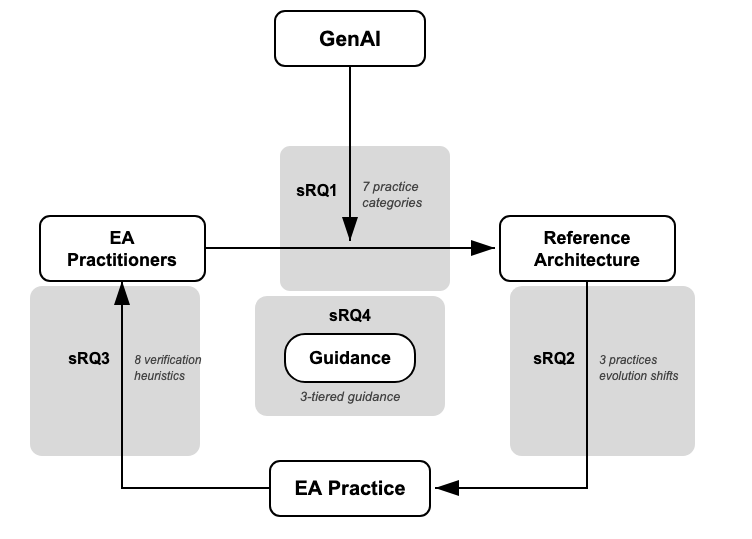
\includegraphics[width=0.75\textwidth]{images/conceptual_model_conclusion.png}
    \caption[Research conclusions mapped to the analytical framework.]{Research conclusions mapped to the analytical framework (cf. Figure~\ref{fig:analytical-framework}).}
    \label{fig:conclusions-framework}
\end{figure}

\textbf{Overall conclusion:} EA practitioners are developing structured,
category-specific practices for GenAI integration, and these practices can be
systematized through consensus-validated guidance that respects the variability
inherent in context-dependent architectural work.

%% ================================================================
%% 7.2 Contributions
%% ================================================================
\subsection{Contributions}\label{subsec:contributions}

Theoretical contributions (extending distributed cognition, practice theory,
and the junior colleague mental model as calibration heuristic) are developed
in Section~\ref{subsec:disc-implications-theory}. Here we summarize the
practical contributions.

\subsubsection{Contributions to Practice}

Five practical contributions emerge from these results. First, the practice
taxonomy describes what practitioners actually do with GenAI, not what the
technology can theoretically do. Each of the seven categories maps to specific
RA development activities and gives organizations a shared vocabulary for
discussing GenAI integration.

Second, the consensus--variability profiles reveal where GenAI adds consistent
value and where its contribution remains contested. System/Codebase Analysis
($M = 4.00$, $SD = 0.82$) represents a zone of reliable augmentation, while
Stakeholder Communication ($M = 3.00$, $SD = 1.37$) marks the organizational
context boundary where GenAI value depends heavily on local conditions.

Third, the guidance artifact offers graduated entry points with embedded
traceability mechanisms (verification heuristics, stakeholder-fit checks, and
trust calibration references) at each practice level. Practitioners new to
GenAI integration can begin with directive-level practices where consensus is
strong, then progress to adaptive practices as they develop calibration skills.
This structure addresses the guidance vacuum identified in
the \textit{Introduction} (Section~\ref{sec:introduction}): the absence of evidence-based
understanding, evaluation frameworks, risk management guidance, and shared
vocabulary for GenAI-augmented EA practice.

Fourth, the gate-to-guardrail governance transition addresses a practical
problem: when anyone with GenAI can produce architectural artifacts, periodic
review boards cannot keep up. Encoding architectural constraints as
machine-readable rules and checking them continuously gives organizations a
governance pathway that scales with GenAI-accelerated artifact production.

Fifth, the anti-atrophy strategies address a concrete risk: practitioners lose
skills they stop exercising, and GenAI automates precisely the skills (cold-start
writing, exhaustive research, cover-to-cover reading) through which architectural
expertise develops \parencite{kabashkin_cognitive_atrophy_2025}. Three friction
strategies (AI-free design sessions, attempt independently first, pair
programming mindset) help practitioners maintain the independent capability that
makes trust calibration possible.

%% ================================================================
%% 9.3 Limitations
%% ================================================================
\subsection{Limitations}\label{subsec:concl-limitations}

\textit{Limitations} (Section~\ref{subsec:disc-limitations}) detailed six categories of limitations
qualifying these findings. Three merit brief restatement here so the conclusion
stands independently. First, the Delphi panel comprised eight to ten
participants drawn from the researcher's professional network, limiting generalizability and introducing self-selection bias toward early
adopters. Second, all findings represent a temporal snapshot from January to
March 2026; GenAI capabilities evolve rapidly, and specific tool-dependent
practices may shift within months. Third, practice data is self-reported through
workbooks and facilitated sessions rather than directly observed, introducing
potential recall and social desirability biases. One additional qualification
bears emphasis: these are early-adopter findings, producing a portrait of
frontier practice that may not generalize to the broader EA practitioner
population as adoption matures.


\clearpage
% Section 08: Discussion
% Mode: Interpretive — "These findings suggest...", "In our view...",
%   "This aligns with \textcite{author}'s concept of..."

\section{Discussion}\label{sec:discussion}

\subsection*{Introduction}

This section interprets the findings from \textit{Results and Analysis} (Section~\ref{sec:results}) and the
guidance artifact from \textit{Guidance Artifact} (Section~\ref{sec:artifact}) against the theoretical
framework established in the \textit{Theoretical Background} (Section~\ref{sec:theoretical-background})
and \textit{Conceptual Model} (Section~\ref{sec:conceptual-model}). Three lenses structure the interpretation:
distributed cognition, practice theory, and the jagged technological frontier.
The section then triangulates the practice catalog against external evidence,
draws implications for Enterprise Architecture (EA) practice and theory, and
closes with limitations and future research directions. The following
subsections detail this interpretation:

\localtableofcontents\clearpage

%% ================================================================
%% 8.2 Distributed Cognition in EA-GenAI Practice
%% ================================================================
\subsection{Distributed Cognition in EA-GenAI Practice}\label{subsec:disc-dcog}

The conceptual model positioned EA-GenAI integration as a distributed cognitive
system where the functional properties of the whole cannot be reduced to the
properties of individual agents \parencite{hutchins_cognition_1995}. The
Delphi findings confirm this
framing while revealing specific distribution patterns that the theoretical
framework anticipated but did not specify.

\subsubsection{Cognitive Distribution Patterns Across Practices}

The seven validated practice categories represent distinct configurations of
cognitive distribution between human and artificial agents. These
configurations align with \textcite{hollan_distributed_2000}'s three types of
distribution (across group members, between internal and external structures,
and through time) though the boundaries are more fluid than the typology
implies.

The Delphi data suggest that System/Codebase Analysis distributes information
retrieval to GenAI while retaining interpretive judgment with the practitioner.
The tight consensus on this practice
(Table~\ref{tab:practice-importance}) suggests that cognitive
distribution succeeds most clearly when the delegated task (scanning code
repositories, mapping dependencies) is verifiable against physical systems.
The trust spectrum for GenAI in RA development (Table~\ref{tab:trust-spectrum}) places information
compression at the highest trust level, consistent with this interpretation.
This convergence implies that verifiability, not task complexity, determines
where cognitive distribution succeeds most readily.

Research \& Exploration appears to distribute information gathering across a
broader knowledge space. The prevalence of Research Assistant mode among Round~1
practices (Section~\ref{subsubsec:practice-discovery}) suggests that
practitioners default to using GenAI to compress
large bodies of information into actionable summaries. This corresponds to
\textcite{hollan_distributed_2000}'s coordination between internal and external
structures: the practitioner's architectural mental model interacts with
GenAI's encoded knowledge to produce synthesis neither could achieve alone.

In a similar vein, First Draft \& Documentation appears to distribute
expression while retaining architectural thinking. The widespread adoption of
the Compression Not Generation framing (Section~\ref{subsubsec:cross-cutting})
captures this distinction precisely. As P3 stated: ``The thinking is still mine; the
AI accelerates expression'' (R1 Workbook). GenAI handles the cognitive labour
of transforming ideas into structured documents; the practitioner retains the
conceptual architecture that gives those documents meaning.

Stakeholder Communication and Governance/Compliance occupy a different position
in the distribution landscape. Both exhibited high variability
(Table~\ref{tab:practice-importance}), and both involve organizational context
that the panel near-unanimously identified as outside GenAI capability
(Section~\ref{subsubsec:cross-cutting}). These findings suggest that cognitive
distribution encounters a boundary at the organizational context interface; a
point we return to below.

\subsubsection{The Organizational Context Boundary}

The most consistent finding across the Delphi study was the organizational
context boundary. The panel near-unanimously identified team dynamics,
political constraints, and historical decisions as knowledge that cannot be
delegated to GenAI (Section~\ref{subsubsec:cross-cutting}). P3 observed that
``organisational context is nearly impossible to convey'' (R1 Workbook), while
P4 noted that GenAI ``is not valuable for the sociotechnical aspects that
determine whether an architecture will actually succeed'' (R1 Workbook).

In our view, this boundary maps directly to
\textcite{hutchins_cognition_1995}'s concept of functional system boundaries.
A distributed cognitive system operates within constraints set by its
participants' capabilities and the media available for coordination.
Organizational context (tacit, political, embedded in history) resists being
translated into forms GenAI can process. The context engineering practices described in
Section~\ref{subsubsec:context-engineering} narrow this boundary by making more
organizational knowledge machine-accessible, but they do not eliminate it.

This interpretation aligns with \textcite{saint-louis_investigation_2019}'s
three contexts of EA practice. The technological context maps readily to
cognitive distribution (System/Codebase Analysis). The socio-technological
context permits partial distribution with human oversight (First Draft \&
Documentation, Adversarial Review). The eco-technological context (external
standards, compliance, regulatory relationships) demands the most careful
verification (Governance/Compliance). An alternative explanation is that this boundary reflects current GenAI
limitations rather than a structural feature; future systems with richer
organizational memory may narrow it. However, the consistency across
all three EA contexts suggests the boundary reflects a structural
feature of distributed cognition in sociotechnical systems, not solely a
technological shortcoming.

\subsubsection{Verification as Cognitive Coordination}

The universal verification mandate (all eight participants described explicit
verification practices, with none accepting GenAI outputs without review
(Section~\ref{subsubsec:cross-cutting})) takes on new significance when viewed
through the distributed cognition lens. Verification is not merely quality
control. It is the mechanism through which the distributed cognitive system
maintains coherence.

\textcite{hutchins_cognition_1995} described how navigation teams use
redundant representations and cross-checking procedures to detect and correct
errors propagating through the cognitive system. The Delphi panel's
verification practices serve an analogous function. The top-tier heuristics (cross-validation, incremental trust building, and
context management; Table~\ref{tab:heuristic-importance}) are cognitive
coordination mechanisms that ensure distributed outputs align with the
practitioner's architectural intent.

The verification burden shift, rated the most significant practice change
(Table~\ref{tab:change-significance}), reflects a
fundamental restructuring of the cognitive system. Practitioners spend less
time on information gathering and expression (now distributed to GenAI) and
more time on coordination and validation. This shift is consistent with
\textcite{hollan_distributed_2000}'s observation that distributed cognitive
systems require coordination overhead proportional to their distribution
complexity.

%% ================================================================
%% 8.3 Practice Evolution Through a Practice Theory Lens
%% ================================================================
\subsection{Practice Evolution Through a Practice Theory Lens}\label{subsec:disc-practice-theory}

The conceptual model drew on \textcite{feldman_theorizing_2011}'s
conceptualization of practice as recurrent, recognizable patterns of action that
emerge through repeated performance. The Delphi findings provide empirical grounding for how
such patterns emerge under conditions of rapid technological change.

\subsubsection{From Creator to Curator: A Sociomaterial Accomplishment}

The creator-to-curator role transformation
(Section~\ref{subsubsec:practice-changes}) represents what
\textcite{orlikowski_sociomaterial_2007} would describe as a sociomaterial
accomplishment. The role shift did not arise from a deliberate redesign of
practice. It emerged through situated interaction between practitioners and
GenAI capabilities.

\textcite{orlikowski_using_2000}'s concept of technology-in-practice
illuminates this process. Practitioners did not adopt GenAI according to a
predefined workflow. Instead, they enacted new practices through ongoing
interaction, discovering that their most productive contribution shifted from
producing architectural content to evaluating, editing, and validating it.
Round~2 confirmed this shift: verification burden received the highest
significance rating, while the creator-to-curator transformation showed
notably higher variability (Table~\ref{tab:change-significance}).

A selection bias caveat applies: practitioners who gravitate toward curation
may be those who adopted GenAI earliest. However, the variability in the
creator-to-curator rating is itself informative.
\textcite{feldman_theorizing_2011} emphasize that practices are constituted
through performance. The uneven adoption of the curator role across the panel
suggests that this transformation is still being constituted, with different
organizational contexts producing different enactments.

\subsubsection{Emergent Practice Patterns}

The seven practice categories exhibit the characteristics
\textcite{feldman_theorizing_2011} identify as constitutive of practice:
recurrence, recognizability, and emergence through repeated performance. None
of the 19 Round~1 practices were formally designed. All arose through
practitioner experimentation with GenAI capabilities in the context of
architectural work. This emergence aligns with the conceptual model's
prediction that ``practices cannot be predicted from GenAI's technical
capabilities alone'' (Section~\ref{sec:conceptual-model}).

The Delphi convergence process itself demonstrated how individual practices
aggregate into collective patterns. Round~1 captured 19 individual practices;
Round~2 synthesized these into seven validated categories; Round~3 refined
heuristics and cross-role dynamics. This progression mirrors the
individual-collective dimension identified in the conceptual framework
(Section~\ref{subsec:frameworkdimensions}): personal experimentation aggregated
into shared organizational patterns through collective deliberation.

\textcite{kotusev_enterprise_2018}'s finding that successful EA practices
diverge substantially from mainstream literature prescriptions resonates
with this emergence pattern. The seven practice categories did not map neatly
onto existing EA frameworks or prescribed GenAI workflows. They emerged from
the complex interplay of practitioner creativity, organizational constraints,
and technological capabilities; precisely the sociomaterial dynamics that
practice theory predicts.

The cross-role dynamics data reinforce this interpretation. All six cross-role
patterns in Table~\ref{tab:cross-role} exhibited variability between 37\% and
79\% (Section~\ref{subsubsec:cross-role}), indicating that practices crossing
traditional role boundaries are still actively being constituted. The ``Ghost
Architect'' provocation surfaced a genuine tension: GenAI democratized artifact
production, yet accountability for architectural decisions remained with the
architect. This asymmetry (distributed production with
concentrated accountability) illustrates the uneven pace at which different
dimensions of practice emerge. \textcite{feldman_theorizing_2011} argue that
practices are constituted through performance; when new actors enter the
performance space, the practice itself must be reconstituted. The high
variability across cross-role patterns suggests that this reconstitution is
underway but far from settled, shaped more by organizational context than by
GenAI capability alone.

\subsubsection{Compression Not Generation as Practice Reframing}

The Compression Not Generation pattern represents a collective reframing of
GenAI's role in architectural practice, adopted by the majority of the panel. As P2 described: ``The value is not in generation
but in compression. It compresses reading time for surveys'' (R1 Workbook).
This framing is significant from a practice theory perspective because it
reveals how practitioners make sense of a new technology in terms compatible
with their existing professional identity.

\textcite{orlikowski_technological_1994}'s concept of technological frames
helps explain this dynamic. By framing GenAI as a compression tool rather than
a generative agent, practitioners maintained their self-understanding as the
source of architectural knowledge. The technology became an accelerator of
human thinking rather than a substitute for it. This framing connects directly
to the role identity preservation pattern: all eight participants viewed GenAI
as an efficiency tool, not a replacement for professional judgment
(Section~\ref{subsubsec:cross-cutting}).

%% ================================================================
%% 8.4 The Jagged Frontier in Architectural Work
%% ================================================================
\subsection{The Jagged Frontier in Architectural Work}\label{subsec:disc-jagged-frontier}

\textcite{dellacqua_navigating_2023} introduced the concept of a ``jagged
technological frontier'' to describe how AI capabilities vary unpredictably
across tasks. Their study of Boston Consulting Group consultants found that
task performance improved substantially when tasks fell inside the frontier
but degraded when they fell outside it. The Delphi consensus--variability
profiles map onto this concept in revealing ways.

\subsubsection{Mapping the Frontier Through Consensus Data}

System/Codebase Analysis sits clearly inside the frontier
(Table~\ref{tab:practice-importance}). The tight consensus and low variability
suggest that organizational context matters less: codebase analysis is
relatively standardized, verifiable, and bounded. This stable frontier boundary
suggests that directive guidance may be feasible.

Research \& Exploration and Adversarial Review occupy the frontier's middle
zone, with moderate consensus supporting contextual guidance, namely general
recommendations with situational qualification. The frontier here depends on
the specificity of the research question and the practitioner's domain
expertise.

Stakeholder Communication and Governance/Compliance sit on or outside the
frontier. Their high variability reflects that GenAI's value for these
practices depends heavily on organizational context; precisely the knowledge
that the panel identified as outside GenAI capability. The shifting frontier
boundary suggests that adaptive guidance may be more appropriate for these
practices.

Deep Workflow Integration presents a different pattern. Its low mean rating
and one abstention likely reflect adoption barriers rather than low frontier
placement. The participants operating in Cyborg mode
(Section~\ref{subsubsec:practice-discovery}) demonstrated that
practitioners who overcome infrastructure prerequisites achieve sustained
workflow benefits. The frontier for this practice may be wide but the path to reaching it is
steep. This suggests that for Deep Workflow Integration, the primary barrier
is organizational readiness rather than GenAI capability.

\subsubsection{Frontier Learning Through Failure}

The majority of participants described learning GenAI's limitations through
errors: hallucinated benchmarks, non-existent folder references, bounded
context suggestions that were ``technically logical but organisationally
nonsensical'' (P3, R1 Workbook). These incidents demonstrate what
\textcite{dellacqua_navigating_2023} describe as the cost of operating outside
the frontier: degraded performance that can propagate downstream if
undetected.

In our view, the frontier learning pattern reveals a distinctive feature of the
EA-GenAI cognitive system. Unlike the BCG consultants in
\textcite{dellacqua_navigating_2023}'s study, who were experimentally assigned
to tasks inside or outside the frontier, EA practitioners must navigate the
frontier continuously in their daily work. The verification heuristics refined
across three Delphi rounds (Table~\ref{tab:heuristic-importance}) represent
collectively developed navigation strategies for this frontier.

The tier structure of verification heuristics reinforces this interpretation.
Process-oriented heuristics (cross-validation, incremental trust building,
context management) rated higher than experience-dependent ones (domain
expertise threshold, learn through failure). This suggests that the panel
valued systematic frontier navigation strategies over individual intuition; a
finding consistent with \textcite{hutchins_cognition_1995}'s emphasis on
procedural coordination in distributed cognitive systems.

\subsubsection{Trust Calibration as Frontier Navigation}

Trust calibration (the bidirectional process of adjusting expectations about
GenAI capabilities) functions as the primary mechanism for navigating the
jagged frontier. The ``junior colleague'' mental model recurred across the
Round~3 panel: ``Think of AI as a junior architect and yourself as the senior
architect'' (R3 Brainstorm). This framing establishes a calibration anchor that
adapts as practitioners accumulate experience with GenAI's capability profile.

The panel confirmed that trust calibration is teachable but requires domain
expertise as a prerequisite (Section~\ref{subsubsec:teachability}). This
finding has implications for the frontier's temporal dimension. Novice
practitioners lack the domain knowledge to recognize when GenAI operates
outside the frontier, making them more vulnerable to the ``beautiful but wrong''
outputs that \textcite{dellacqua_navigating_2023} identified. The experience
indicators in the guidance artifact (Section~\ref{subsec:practice-catalog})
address this by providing graduated entry points for practitioners at different
experience levels.

%% ================================================================
%% 8.5 External Triangulation of Delphi Practices
%% ================================================================
\subsection{External Triangulation of Delphi Practices}\label{subsec:disc-triangulation}

The guidance artifact in Section~\ref{sec:artifact} is grounded in the Delphi
study. This section examines how external evidence corroborates, extends, or
qualifies the seven validated practice categories. The purpose is triangulation:
establishing whether the Delphi findings reflect broader practitioner experience
or remain idiosyncratic to this panel.

\textbf{System/Codebase Analysis.} Practitioner evidence confirms codebase
analysis as the highest-confidence GenAI application. Practitioners report using
GenAI for reverse-engineering software architecture, producing dependency graphs
and cross-repository documentation
\parencite{chatlatanagulchai_agent_readmes_2025}. Agent context files containing
architecture content appear in 67.7\% of analyzed repositories, indicating
widespread adoption of this practice in tooling-integrated workflows. This
convergence strengthens the directive guidance level assigned to this practice.

\textbf{Research \& Exploration.} Multi-model research pipelines are emerging,
where practitioners use different AI models for planning, structuring, and
execution stages \parencite{banh_affordance_genai_ea_2025}. The compression
framing (GenAI compresses existing information rather than creating new
knowledge) is well-established in practitioner discourse and aligns with the
Delphi finding that five of eight participants adopted this framing
(Section~\ref{subsubsec:cross-cutting}). External evidence thus corroborates
both the practice and its underlying cognitive model.

\textbf{Adversarial Review / Stress Testing.} The adversarial use of GenAI is
documented across practitioner discourse, though primarily as informal validation
rather than structured architectural critique
\parencite{lee_devils_advocate_2025, stanimirovic_ai_sparring_2026}. Epistemic
stress testing (tracking confidence levels in AI-mediated architectural
decisions) connects to the distributed cognition lens by making cognitive
assumptions explicit \parencite{gilda_epistemic_status_2026}. The stress testing
techniques identified in Table~\ref{tab:stress-testing} draw on both Delphi data
and this external evidence.

\textbf{Governance/Compliance.} The gap between governance aspiration and
implementation is well-documented.
\textcite{ettinger_ea_dynamic_capability_2025} identifies significant
limitations in existing EA frameworks for addressing GenAI requirements, noting
tension between fostering innovation and maintaining compliance.
Architecture-as-Code approaches (encoding architectural constraints as
machine-readable rules in CI/CD pipelines) represent an emerging response to this
gap \parencite{bucaioni_architecture_as_code_2025}. The high variability in the Delphi rating
(Table~\ref{tab:practice-importance}) is consistent with this literature:
governance value depends heavily on organizational maturity.

\textbf{First Draft \& Documentation.} This practice has the strongest external
corroboration. Practitioners report generating architecture decision records from
meeting transcripts and requirements, with multi-layer verification workflows
combining metaprompts, fresh LLM contexts, and LLM-as-Judge evaluation before
human review \parencite{banh_affordance_genai_ea_2025}. The verification burden
shift (the highest-rated change theme,
Table~\ref{tab:change-significance}) is most directly experienced in
documentation workflows. A related emerging practice, Spec-Driven Development
(SDD), extends the documentation-first principle by using formal specifications
as the primary human-authored artifact from which implementations derive
\parencite{piskala_spec_driven_dev_2026}. SDD is not yet a validated Delphi
practice, but its specification-anchored approach mirrors how RAs function:
normative specifications constraining downstream implementation. Early evidence
suggests three maturity levels (spec-first, spec-anchored, and spec-as-source),
though concerns about specification drift and tool inflexibility remain
\parencite[sec.~IX]{piskala_spec_driven_dev_2026}.

\textbf{Stakeholder Communication.} External evidence for GenAI-assisted
stakeholder communication in architecture contexts is sparse compared to other
practices. The strongest evidence concerns meeting transcript synthesis into
formal records (collective decision capture received the highest cross-role
pattern rating, Table~\ref{tab:cross-role}) rather than proactive
stakeholder communication. This evidence gap is consistent with the practice's
high variability and adaptive guidance level.

\textbf{Deep Workflow Integration.} The shift from chat-based interaction to
IDE-integrated workflows represents a maturation trajectory documented across
practitioner discourse \parencite{rajasekaran_context_engineering_2025,
chatlatanagulchai_agent_readmes_2025}. Agent context files containing
architecture content appear in 67.7\% of studied repositories, and enterprise
organizations are converting internal APIs into MCP servers at scale. Context
engineering (designing the information environment for AI agents) is emerging as
a core architectural skill (Section~\ref{subsubsec:context-engineering}).

Taken together, external evidence corroborates the Delphi findings across all
seven practice categories, though with varying strength. System/Codebase
Analysis and First Draft \& Documentation have the strongest external
validation, consistent with their higher consensus ratings. Stakeholder
Communication and Deep Workflow Integration have sparser external evidence,
consistent with their adaptive guidance levels. This pattern suggests that
the Delphi panel's consensus--variability profiles reflect genuine differences
in practice maturity rather than panel idiosyncrasy.

%% ================================================================
%% 8.6 Implications for EA Practice
%% ================================================================
\subsection{Implications for EA Practice}\label{subsec:disc-implications-practice}

The theoretical interpretations above yield four practical implications for
how EA practice may evolve as GenAI integration matures.

\subsubsection{Context Engineering as an Emerging Competency}\label{subsubsec:disc-context-eng}

The Delphi findings position context engineering (systematically designing
the information provided to GenAI systems) as an emerging EA competency.
The strong panel endorsement of the context management heuristic
(Table~\ref{tab:heuristic-importance}), combined with the finding that
agent context files containing architecture content appear in 67.7\% of
studied repositories \parencite{chatlatanagulchai_agent_readmes_2025},
indicates that context engineering is not merely aspirational but reflects
emerging practice maturity. These files function as both human-readable
documentation and machine-executable constraints.

Context engineering extends the traditional EA practitioner
competency set identified by \textcite{land_enterprise_2009} (which
emphasized technical expertise, communication skills, and political
acumen) with a new dimension. That dimension is the ability to represent
architectural knowledge in forms that GenAI systems can process
effectively. This is not
merely a technical skill. It requires the architectural judgment to determine
which constraints matter, the communication skill to encode them precisely,
and the organizational awareness to know what context the AI lacks.

\subsubsection{The Gate-to-Guardrail Transition}

The governance adaptation themes in Section~\ref{subsec:governance-adaptation}
suggest a shift from periodic gate reviews to continuous guardrail enforcement.
GenAI's acceleration of artifact production (practitioners producing drafts in
minutes rather than days) challenges the temporal assumptions of traditional
architectural review boards. The Delphi panel's low rating for inside-out governance
(Table~\ref{tab:cross-role}) suggests that most organizations have not yet
confronted this shift.

\textcite{ettinger_ea_dynamic_capability_2025} identifies significant
limitations in existing EA frameworks for addressing GenAI requirements. In our
view, the gate-to-guardrail transition represents the governance equivalent of
cognitive distribution: encoding architectural constraints as machine-readable
rules distributes governance enforcement across the development pipeline rather
than concentrating it in periodic human reviews. This transition directly
addresses the accountability gap exposed by the Ghost Architect dynamic
(Section~\ref{subsubsec:cross-role}): when artifact production is distributed
but accountability remains concentrated, continuous guardrail enforcement shifts
evaluation from \textit{who produced} the artifact to \textit{whether it meets
encoded standards}. In this way, the gate-to-guardrail model resolves the
asymmetry between distributed production and concentrated accountability by
making compliance verifiable regardless of the artifact's origin.

\subsubsection{The Competency Decay Paradox}

The skills being automated (cold-start writing, exhaustive manual search,
cover-to-cover documentation reading) are the same skills through which
practitioners built their expertise
\parencite{kabashkin_cognitive_atrophy_2025}. The panel rated ``skills used less'' as the second-most significant change
(Table~\ref{tab:change-significance}), confirming that practitioners recognize
this dynamic. Yet ``new skills emerging'' received a notably lower rating,
suggesting practitioners perceive the shift as extending existing expertise
rather than requiring fundamentally new competencies.

This tension reveals a paradox that practice theory helps illuminate. If
practices are constituted through performance
\parencite{feldman_theorizing_2011}, then automating the performance
undermines the mechanism through which expertise develops. Future practitioners
may lack the foundation required for effective trust calibration; precisely
the skill the panel identified as essential for all seven practices.

The anti-atrophy strategies proposed in
Section~\ref{subsubsec:anti-atrophy} constitute a practice-theoretic response
to this paradox. If expertise develops through performance
\parencite{feldman_theorizing_2011}, then preserving expertise requires
deliberately reintroducing the performance that automation displaces. Each
strategy targets a different facet of this mechanism. AI-free design sessions
preserve foundational skill performance by requiring practitioners to produce
architectural work without GenAI assistance. The attempt-independently-first
protocol maintains mental model formation by ensuring practitioners engage with
problems before encountering AI-generated representations. The pair programming
mindset sustains active cognitive engagement during GenAI-assisted work,
preventing delegation from becoming abdication. These strategies
represent deliberate friction: a structured reintroduction of the cognitive
effort that constitutes architectural expertise.

\subsubsection{The Maturity Model as Diagnostic}

The four-stage maturity model (Table~\ref{tab:maturity-model}) received partial
empirical support through the asynchronously collected SP2 maturity progression
vote (Table~\ref{tab:maturity-progression}). The panel strongly endorsed the natural progression assumption while rejecting
the proposition that short experience can substitute for sustained engagement
(Table~\ref{tab:maturity-progression}). The model's value remains diagnostic rather than prescriptive. Practitioners can
use it to locate their current practice and identify potential growth areas
without implying that progression through all four stages is necessary or
desirable for every organizational context.

The SP2 results reveal a nuanced position that echoes a broader debate in EA
maturity literature. \textcite{kotusev_enterprise_2018} demonstrated that EA
maturity models often prescribe trajectories that bear little resemblance to how
practices actually evolve. The panel's moderate, high-variability agreement on per-category measurement
and context-dependence aligns with this critique: progression is real but not
uniform across practice categories. The high variability across organizational contexts
(particularly in Governance/Compliance and Stakeholder Communication) further
suggests that context-specific factors shape adoption pace more than any
universal progression logic. The specific four-stage structure remains
researcher-proposed, and the asynchronous collection mode introduces
methodological caveats (Section~\ref{subsec:data-limitations}).

%% ================================================================
%% 8.6 Implications for Theory
%% ================================================================
\subsection{Implications for Theory}\label{subsec:disc-implications-theory}

The findings extend three theoretical areas: distributed cognition, practice
theory, and the conceptualization of GenAI in professional knowledge work.

\subsubsection{GenAI as Cognitive Partner}

Distributed cognition theory \parencite{hutchins_cognition_1995} originally
examined how cognitive processes distribute across human team members and
physical artifacts. The Delphi findings suggest that GenAI occupies a position
in the cognitive system distinct from both. The organizational context
boundary, near-unanimously identified as a hard limit on delegation
(Section~\ref{subsubsec:cross-cutting}), delineates where GenAI's
cognitive partnership reaches its current limits. Yet within that boundary,
practitioners described GenAI generating novel representations, responding to
queries contextually, and adapting outputs to conversational framing;
capabilities that exceed those of the charts, instruments, and procedures in
\textcite{hutchins_cognition_1995}'s navigation studies. In our view, GenAI
functions as a new category of cognitive partner: more capable than a static
artifact but less reliable than a human collaborator in domains requiring
tacit organizational knowledge.

These findings point toward a pattern not explicitly addressed in
\textcite{hollan_distributed_2000}'s three types of distribution: distribution
to agents whose reliability varies across task types. The consensus--variability
profiles from Section~\ref{subsec:disc-jagged-frontier} offer preliminary
indications of this pattern. The tight consensus on System/Codebase Analysis suggests relatively stable
perceived reliability, while the wide disagreement on Stakeholder Communication
suggests less predictable performance. These variability differences reflect
panel-level variation in importance ratings rather than direct measures of
GenAI reliability. Yet the
pattern they trace is consistent with the jagged frontier
\parencite{dellacqua_navigating_2023}, where AI capability varies
unpredictably across task boundaries. While the present study's scope does not
permit theoretical generalization, the observation warrants further
investigation. Distributed cognition theory, as originally formulated, assumed
relatively stable capabilities among system components. GenAI may introduce a
partner whose competence shifts across task boundaries, requiring continuous
calibration; a dynamic the original framework did not anticipate.

\subsubsection{Practice Emergence Under Rapid Technological Change}

\textcite{feldman_theorizing_2011}'s practice theory provides a lens for
understanding how recurrent patterns of action emerge and stabilize. The Delphi
findings illustrate a distinctive feature of practice emergence under rapid
technological change: the technology's capabilities shift faster than practices
can stabilize.

The seven practice categories validated in Round~2 showed no challenges or
revisions in Round~3 (Section~\ref{subsubsec:convergence}), suggesting that
the practice taxonomy itself has stabilized. However, the specific
enactments within each category (the tools used, the verification strategies
applied, the interaction patterns adopted) continue to evolve as GenAI
capabilities advance. This creates what we might describe as stable categories
with fluid content: the practice patterns are recognizable but their
instantiation changes continuously.

\textcite{orlikowski_using_2000} argued that technology-in-practice emerges
through situated use rather than following predetermined adoption paths.
The Delphi findings support this claim but add a temporal dimension: when
the technology itself evolves rapidly, practitioners must continuously
re-situate their practices. The frontier learning pattern (the majority of participants discovering
limitations through errors) demonstrates this ongoing re-situation in action.

\subsubsection{The Junior Colleague Mental Model}

The ``junior colleague'' framing, recurrent across the Round~3 panel, deserves
theoretical attention as a novel calibration heuristic. One participant
stated: ``Think of AI as a junior architect and yourself as the senior
architect'' (R3 Brainstorm). Another described treating GenAI interaction like
a buddy system where ``sharing the elements as if it were human betters the
end output'' (R3 Brainstorm).

This mental model is not a formal theoretical contribution but a practitioner
heuristic that performs important cognitive work. It establishes appropriate
expectations (capable but requiring supervision), defines the appropriate
relationship (mentorship rather than delegation or replacement), and provides
a familiar frame of reference for navigating an unfamiliar technology.

In our view, the junior colleague model is theoretically significant because
it reveals how practitioners make sense of a novel cognitive partner by drawing
on social frameworks from human collaboration. This process (making the
unfamiliar familiar through analogical reasoning) represents a sense-making
strategy that existing literature on GenAI adoption has not foregrounded. The
framing also reveals its own limitations. Unlike a junior colleague, GenAI
does not learn from supervision in ways that transfer across sessions. Its
failure modes also differ fundamentally from those of a human novice.

%% ================================================================
%% 8.7 Limitations
%% ================================================================
\subsection{Limitations}\label{subsec:disc-limitations}

Several limitations qualify the findings and their interpretation.

\textbf{Sample size and composition.} The Delphi panel comprised eight to ten
participants across three rounds, sufficient for a Delphi study targeting information richness but limiting
generalizability. The panel was
predominantly European, self-selected through the researcher's professional
network, and composed of practitioners already using GenAI. This composition
produces a portrait of early adopter practices that may not represent the
broader EA practitioner population.

\textbf{Scope boundary tension.} The workbook was framed as ``Software
Architecture / Solution Design work'' rather than ``Enterprise Architecture'' to
capture practitioners who do RA work under various professional labels (see
Section~\ref{sec:methodology}). This terminological broadening may have
admitted practices that sit at the boundary between RA-specific and general
architectural work. The workbook's RA lifecycle mapping (Part~C) and R2's
RA-contextualized validation mitigate this risk, but some practices (e.g.,
System/Codebase Analysis) may represent general architectural work that is not
exclusive to RA development. This is an inherent trade-off: ecological validity
(capturing how practitioners actually describe their work) versus strict
construct alignment with the research question's ``EA practitioners'' scope.
Future research could isolate RA-specific practices from general architectural
practices through comparative studies across different architectural artifact
types.

\textbf{Temporal snapshot.} Data collection occurred between January and March
2026, during a period of rapid GenAI capability evolution. Findings represent
a snapshot of practice at a specific moment. GenAI capabilities available
during the study period (including large context windows, multi-modal
reasoning, and agent-based workflows) may shift substantially within months,
potentially rendering specific findings (particularly tool-dependent practices
like Deep Workflow Integration) outdated.

\textbf{Partially validated maturity model.} The four-stage maturity model
(Table~\ref{tab:maturity-model}) was derived from observed variation in the
Delphi data. The asynchronously collected SP2 vote
(Table~\ref{tab:maturity-progression}) provides empirical support for the underlying progression assumption
($M = 4.71$, variability 22\%), partially grounding a maturity model within a
consensus-based study. However, a residual design-science tension remains: the specific
four-stage structure (from Experimental to Organizational Embedding) was not
individually validated by the panel, the vote was collected asynchronously
without preceding group discussion, and the sample comprised seven participants.
Future research should validate the specific stage boundaries and
characteristics.

\textbf{Delphi process constraints.} Three rounds may limit the depth of
convergence achievable. Round~1's asynchronous format allowed thoughtful
individual responses but prevented the real-time probing possible in
interviews. Rounds~2 and~3 compressed discussion into 120-minute sessions,
with Round~3 Step~15 not executed and Step~16 collected asynchronously. The
absence of Step~15 (Future Perspectives) means the temporal dimension and
future-oriented perspectives of the conceptual framework remain empirically
underexplored.

\textbf{Researcher positionality.} The researcher is an EA practitioner who
uses GenAI daily for architectural work. This dual role means the researcher
is simultaneously a research subject and the person designing the inquiry.
Insider status touched every phase of the research: the discovery workbook
drew on practitioner knowledge of EA workflows, coding decisions reflected
familiarity with architectural reasoning patterns, the seven practice
categories emerged through researcher synthesis of participant data, and the
guidance artifact incorporated the researcher's understanding of what
practitioners would find actionable. Each of these steps involved interpretive
judgments that insider knowledge could shape, creating a structural bias toward
validating the significance of GenAI integration.

Assumption management relied primarily on the Delphi method's structural
safeguards rather than a rigorous personal reflexivity protocol. We acknowledge
that the researcher's actual reflexive practice was less systematic than
planned; reflexive notes were captured at key decision points rather than
maintained as a continuous journal. Three structural features partially
compensated for this gap. Round~1's asynchronous workbook format ensured
participants articulated practices in their own terms before researcher coding
began. Round~2's live voting and discussion allowed the panel to validate or
reject practice categories collectively, not through researcher judgment alone.
Round~3's structured brainstorming generated participant responses that were
aggregated before researcher synthesis. In our view, these deliberative
safeguards provided meaningful protection against insider bias, but we
acknowledge that a more disciplined personal reflexivity practice would have
strengthened confirmability.

Two reflexive insights merit disclosure. The researcher has experimented with
large language models since 2017 and assumed that most EA practitioners would
gradually incorporate GenAI over time. The genuine surprise was the speed of
conversion: several participants described themselves as recently skeptical,
believing EA work was too context-heavy for AI assistance, yet had rapidly
become active daily users within months. This challenged the researcher's
gradualist assumption and highlighted the threshold-crossing pattern visible in
the findings. Regarding the ``Ghost
Architect'' provocation, this stimulus emerged primarily from the data rather
than insider projection. Rounds~1 and~2 surfaced unanticipated cross-role
dynamics, including developers producing architectural artifacts bottom-up
(Section~\ref{subsubsec:cross-role}). The provocation was designed to probe
these participant-identified tensions in Round~3. We acknowledge that insider
status likely influenced the salience assigned to role boundary shifts; an
active practitioner may notice such dynamics more readily. However, the
provocation's content was anchored in participant-generated themes rather than
researcher preconceptions.

\textbf{GenAI tool dependency.} Findings are shaped by the GenAI tools
available in 2025--2026, including large language models from major providers,
IDE-integrated coding assistants, and early agent-based workflows. The
practices, heuristics, and governance considerations identified may not
transfer directly to future GenAI paradigms with different capability profiles.

%% ================================================================
%% 8.8 Future Research
%% ================================================================
\subsection{Future Research}\label{subsec:future-research}

Five directions merit investigation. First, longitudinal research should track
how the seven practice categories evolve as GenAI capabilities advance, since
the temporal snapshot limitation means that practices documented here may
fragment, merge, or transform as tool capabilities shift.

Second, cross-organizational validation of the practice taxonomy would establish
whether the categories identified in this early-adopter panel hold across
different organizational contexts, governance maturity levels, and industry
sectors. Replication studies with larger panels would test whether the consensus
patterns observed here generalize beyond this exploratory sample.

Third, the maturity model's progression assumption received strong panel support
($M = 4.71$), but three areas warrant further validation: the specific four-stage
structure (from Experimental to Organizational Embedding) was not individually
tested, the practice-category-specific nature of maturity suggested by the panel
implies different progression trajectories per practice may exist, and the
model's applicability beyond the early-adopter population studied here remains
unknown.

Fourth, sector-specific RA contexts (healthcare, financial services, government)
introduce regulatory and compliance dimensions that may reshape which
practice categories dominate and how verification heuristics are calibrated.

Fifth, the anti-atrophy strategies proposed in
Section~\ref{subsec:disc-implications-practice} require longitudinal validation.
While this study identifies the competency decay paradox and proposes deliberate
friction interventions, their long-term effectiveness in preserving
architectural expertise remains an open empirical question with significant
implications for EA education and professional development.

%% ================================================================
%% 8.9 Closing Statement
%% ================================================================
\subsection{Closing Statement}\label{subsec:closing-statement}

The research began with a practice vacuum: EA practitioners were integrating
GenAI into RA development without empirical evidence, evaluation frameworks,
shared vocabulary, or validated guidance.
\textcite{kotusev_enterprise_2018} called for reconceptualizing EA practice to
reflect how architects actually work; GenAI has made that call urgent. Through
three Delphi rounds, this study maps what practitioners are doing, how their
work is changing, and what guidance helps. The practices documented here will
evolve as GenAI capabilities advance. What persists is the underlying question:
which parts of architectural work to delegate, and which to keep.


\clearpage
\appendix
% Appendix formatting:
% - Section heading shows: "A  Appendix - Title"
% - PDF bookmark/TOC shows: "A  Appendix - Title"
% Keep \thesection clean for hyperref; use \titleformat for display.
\titleformat{\section}
  {\normalfont\fontsize{16}{19}\bfseries}
  {\Alph{section}\quad Appendix\enspace{}-\enspace{}}{0pt}{#1}
\titlespacing{\section}{0pt}{12pt}{12pt}
\renewcommand{\thesubsection}{\Alph{section}.\arabic{subsection}}
\renewcommand{\sectionmark}[1]{%
  \markboth{Appendix \thesection.\ \ #1}{}%
  \thispagestyle{sectionfirst}%
  \global\currentheadrulewidth=0pt\relax
  \global\currentfootrulewidth=0pt\relax}

\clearpage
\section[Appendix - Use of Generative AI in Research]{Use of Generative AI in Research}\label{app:genai}

This appendix documents what Generative AI (GenAI) tools were used in this
research, how they were deployed, and what functions they served.

Four GenAI systems supported this research:

\begin{enumerate}
    \item Perplexity: For literature discovery and initial source identification
    \item Anthropic Claude: For critical analysis of reading notes, validation of
          guidance artifact outputs, generation of the machine-readable YAML
          companion,\footnote{\url{https://github.com/thiagoavadore/thesis_2024-2026_antwerp_thesis_GenAIPracticeVacuum/blob/main/guidance-artifact.yaml}} front cover prompt design,
          and thesis revision assistance
    \item Meta Llama 3 (self-hosted instance): For critical analysis of reading notes
    \item Google Gemini: For front cover image generation
\end{enumerate}

These tools served six functions:

\begin{enumerate}
    \item \textbf{Efficiency in discovery}: Accelerated identification of relevant
          sources across disciplines;
    \item \textbf{Critical examination}: Provided external perspective on blind spots
          and gaps in interpretation;
    \item \textbf{Research alignment}: Helped assess literature relevance to evolving
          research questions;
    \item \textbf{Artifact validation}: Checked practitioner checklist cards for
          internal consistency, completeness against Section~\ref{sec:artifact}
          content, and formatting;
    \item \textbf{Format generation}: Produced the machine-readable YAML guidance
          artifact from researcher-authored content;
    \item \textbf{Image generation}: Produced the front cover image from a
          researcher-designed concept.
\end{enumerate}

The following sections document each usage in detail.

\subsection{Literature Discovery Process}

Perplexity helped identify relevant literature beyond traditional academic
search engines (Google Scholar) and supervisor recommendations.

\textbf{Example discovery prompt}: \textit{In the context of Software and Infrastructure engineering,
    are there any peer-reviewed articles/papers that connect Reference Architecture and tools that
    support it, including AI tools? If so, give me a list with sources. This is for academic research,
    so explore and reference only journals, thesis and dissertations - skip the blog posts.}

\subsection{Literature Review Process}

The review process followed a three-stage pattern:

\begin{enumerate}
    \item \textbf{Reading and Note-Taking}: Papers identified through discovery were added to
          Zotero and read systematically. Notes captured key points, learnings, questions,
          and findings.
    \item \textbf{Critical Analysis}: Notes were submitted to GenAI systems for critical
          examination using the following prompt:

          \textit{I've read the paper (attached) and took notes (also attached) by trying to summarize
              interesting points, learnings, questions and findings. Investigate potential blind spots,
              contradictions or any type of hand-waving on my notes. Critique my points and avoid
              agreeing with me for the sake of making me happy. If the article publication date is before
              your cut training date, investigate what theories and implications it had that are not
              highlighted in my notes, always giving me link to sources.}

    \item \textbf{Research Alignment}: Once the Problem Statement and Research Questions
          crystallized, the analysis prompt evolved to include research alignment:

          \textit{As part of my Executive MSc I'm researching into this Problem Statement/Research
              Question (attached). To better investigate it, I've read the paper (attached) and I
              took notes (also attached) by trying to summarize interesting points, learnings, questions
              and findings. Investigate potential blind spots, contradictions or any type of hand-waving
              on my notes. Critique my points and avoid agreeing with me for the sake of making me happy.
              If the article publication date is before your cut training date, investigate what theories
              and implications it had that are not highlighted in my notes, always giving me link to sources.
              And lastly, investigate if the article supports, contradicts or adds new information to
              the Problem Statement or the Research Question.}

\end{enumerate}

\subsection{Guidance Artifact Preparation}

Two outputs in the appendices involved GenAI assistance:

\begin{enumerate}
    \item \textbf{Practitioner Checklist Cards (\ref{app:checklists}):} The checklist cards were
          researcher-authored based on Delphi findings and the guidance artifact in
          Section~\ref{sec:artifact}. GenAI (Claude) was used to validate the cards for internal
          consistency, completeness against Section~\ref{sec:artifact} content, and formatting. GenAI
          did not generate the card content.
    \item \textbf{YAML Guidance Artifact:} The machine-readable YAML companion
          (available in the research repository\footnote{\url{https://github.com/thiagoavadore/thesis_2024-2026_antwerp_thesis_GenAIPracticeVacuum/blob/main/guidance-artifact.yaml}}) was generated by GenAI (Claude) from the
          researcher-authored Section~\ref{sec:artifact} and checklist card content. The researcher
          reviewed, corrected, and approved the output. This constitutes a format
          transformation of existing researcher-authored material, not new content
          generation.
\end{enumerate}

\subsection{Thesis Revision}

During the final revision phase, Claude (Anthropic) assisted with mechanical
verification tasks: identifying misformatted cross-references after structural
reorganization and verifying APA citation consistency. In all cases, the
researcher reviewed the identified issues and applied corrections manually.

\subsection{Front Cover Image}

The researcher designed the front cover concept to represent the thesis theme
visually: cognitive work (represented by an anatomical brain) transforming into
an architectural blueprint through a verification lens. Three design constraints
guided the concept. First, the image had to be monochromatic to avoid dominating
the page. Second, the transformation had to show intentional loss and change in
the process, reflecting how GenAI outputs require curation rather than blind
acceptance. Third, the style had to match the scholarly tone of an academic
thesis.

Anthropic Claude translated these constraints into a structured image generation
prompt. Google Gemini then generated the image from the following prompt:

\textit{Monochromatic grayscale academic illustration, no text, no letters, no
words, no numbers. A detailed anatomical human brain on the left side, drawn in
fine ink lines, partially dissolving into geometric particles and dots that drift
rightward. These particles gradually reassemble into an abstract architectural
blueprint floorplan on the right side, shown as precise technical line drawings
of rooms, corridors, and structural elements. Between the brain and the
blueprint, a translucent magnifying lens floats, refracting the particles
passing through it, symbolizing verification and curation. Subtle watercolor ink
splashes in light gray behind both elements. Small geometric shapes (circles,
hexagons, connection nodes) scattered in the transition zone. Style: scientific
illustration meets architectural drawing, similar to academic thesis cover art.
White background, no color, purely grayscale ink and pencil aesthetic. High
detail, scholarly tone.}

\subsection{What GenAI Did Not Do}

GenAI tools did not:

\begin{enumerate}
    \item Generate original thesis argumentation or theoretical analysis;
    \item Make methodological decisions;
    \item Conduct analysis of primary research data;
    \item Assist with between-round synthesis, including data coding, taxonomy
          development, or preparation of subsequent round materials;
    \item Develop the conceptual framework;
    \item Independently interpret supervisor feedback.
\end{enumerate}

All interpretation, synthesis, framework development, and argumentation is
the researcher's own work.

\clearpage
\section[Appendix - Discovery Workbook Instrument]{Discovery Workbook Instrument}\label{app:workbook}

This appendix reproduces the complete Round~1 discovery workbook distributed to
participants in January 2026. The workbook comprises seven parts (A--G) that
progress from context setting through practice discovery to reflective
sensemaking.

\textbf{Part A: Context Setting}

This opening section establishes the participant's GenAI context and experience
level:
\begin{itemize}
    \item Which GenAI tools do you currently have access to? (e.g., ChatGPT, Claude,
          Copilot, Gemini, internal tools)
    \item How long have you been experimenting with GenAI in your EA work?
    \item What triggered you to start using GenAI for Reference Architecture development?
    \item Describe your organizational context for EA practice
\end{itemize}

\textbf{Part B: Practice Archaeology}

The core discovery section employs multiple prompts to excavate practices from
different angles:

\textbf{B.1 Genesis Moments}\\
``Think back to the last 3 Reference Architectures you've worked on. Walk through a typical RA development effort.
At what points did you think `maybe GenAI could help here'? What did you actually try?''

\textbf{B.2 Practice Inventory}\\
``Now systematically review your GenAI use. For EACH distinct way you use GenAI, please document:''
\begin{enumerate}[label=B.2.\arabic*]
    \item What do you call this practice? (give it a name)
    \item What problem does it solve?
    \item Describe exactly what you do (step-by-step process)
    \item What specific prompts or techniques have you developed?
    \item How did you discover or develop this approach?
    \item What percentage of the time does it work effectively?
    \item What are the typical failure modes?
\end{enumerate}

Participants documented two to five core practices using this structure.

\textbf{Part C: Lifecycle Positioning}

Participants receive a standard RA lifecycle model \textit{without any GenAI
    annotations}:
\begin{enumerate}
    \item Stakeholder Analysis \& Requirements Gathering
    \item Current State Analysis
    \item Pattern Identification \& Abstraction
    \item Target State Design
    \item Component Specification
    \item Documentation \& Communication
    \item Validation \& Review
    \item Evolution \& Maintenance
\end{enumerate}

For each phase, participants answer:
\begin{itemize}
    \item Which of your named practices apply in this phase?
    \item What percentage of this phase involves GenAI assistance?
    \item What tasks MUST remain human-performed? Why?
    \item What surprised you about GenAI's capabilities or limitations here?
\end{itemize}

\textbf{Part D: Critical Incidents}

``Share 3-5 specific stories where GenAI significantly impacted your RA work (positive or negative).''

For each incident, participants provide:
\begin{itemize}
    \item \textbf{Context}: What were you trying to accomplish?
    \item \textbf{Action}: Exactly what did you do with GenAI?
    \item \textbf{Result}: What happened? (intended and unintended outcomes)
    \item \textbf{Insight}: What did this teach you about using GenAI for RA work?
    \item \textbf{Evidence}: Can you share specific prompts and outputs? (anonymized as needed)
\end{itemize}

\textbf{Part E: Impact Reflection}

\textbf{E.1 Time and Effort Analysis}
\begin{enumerate}[label=E.1.\arabic*]
    \item Estimate hours spent on your last RA with vs. without GenAI
    \item Count iteration cycles needed with GenAI assistance
    \item Identify where GenAI saved time
    \item Identify where GenAI required additional time investment
\end{enumerate}

\textbf{E.2 Quality and Completeness Assessment}\\
``Comparing GenAI-assisted RAs to traditionally developed ones:''
\begin{enumerate}[label=E.2.\arabic*]
    \item What aspects show improved quality? Why?
    \item What aspects show degraded quality? Why?
    \item What is simply different rather than better or worse?
\end{enumerate}

\textbf{E.3 Role Evolution}\\
``How has YOUR role as an EA practitioner changed?''
\begin{enumerate}[label=E.3.\arabic*]
    \item Skills you use more frequently now
    \item Skills you use less frequently now
    \item New skills you've had to develop
    \item What would happen to your practice if GenAI disappeared tomorrow?
\end{enumerate}

\textbf{Part F: Challenges and Workarounds}

``Document obstacles you've encountered using GenAI for Reference Architecture development.''

For each challenge:
\begin{itemize}
    \item Describe the specific problem
    \item Explain your workaround (if any)
    \item Identify what capability you wish GenAI possessed
    \item Note any red flags you've learned to recognize
\end{itemize}

\textbf{Part G: Emergent Wisdom}

``Based on your experience so far:''
\begin{itemize}
    \item What essential advice would you give an EA colleague starting with GenAI
          tomorrow?
    \item What critical mistakes should they avoid?
    \item What's your most counterintuitive discovery about GenAI in RA work?
    \item Where do you predict GenAI use in RA development will be in 12 months?
\end{itemize}

\clearpage
% Appendix C: Practitioner Checklist Cards
% Condensed, scannable reformatting of Section 07 (Guidance Artifact)
% Each card fits approximately one page

\section[Appendix - Practitioner Checklist Cards]{Practitioner Checklist Cards}\label{app:checklists}

This appendix condenses the guidance artifact (Section~\ref{sec:artifact}) into
twelve scannable checklist cards. Each card traces directly to a specific
subsection of the artifact; no new content is introduced. Practitioners may
photocopy or print individual cards for use during Reference Architecture (RA)
development sessions. For Cards~1--7, practice descriptions and verification
patterns carry Delphi consensus; experience indicators (Novice/Advanced) are
researcher proposals.

%% ================================================================
%% Card 1: System/Codebase Analysis
%% ================================================================
\clearpage
\subsection*{Card 1: System/Codebase Analysis \hfill \textit{[Directive]}}

\begin{tabular}{|p{7cm}|p{6cm}|}
    \hline
    \textbf{Consensus:} $M = 4.00$, $SD = 0.82$ & \textbf{Provenance:} Delphi consensus \\
    \hline
\end{tabular}

\vspace{0.5em}
\textbf{When to Use}
\begin{itemize}
    \item Phase~2 (Current State Analysis) of the RA lifecycle
    \item Legacy system comprehension, dependency mapping, cross-repository analysis
\end{itemize}

\textbf{Key Steps}
\begin{enumerate}
    \item Feed existing system artifacts (code, configs, diagrams) into GenAI for analysis
    \item Delegate information gathering to GenAI; retain architectural judgment
    \item Cross-validate GenAI-generated descriptions against source systems directly
    \item Verify that referenced components, services, and dependencies exist in the actual system
\end{enumerate}

\textbf{Verification Checklist}
\begin{itemize}[label=\checkbox]
    \item Cross-validate system descriptions against source systems (Trust level: Highest)
    \item Confirm referenced folders, components, and services exist physically
    \item Verify dependency graphs against actual system topology
    \item Spot-check representative samples of information compression outputs
\end{itemize}

\begin{tabular}{|p{6.5cm}|p{6.5cm}|}
    \hline
    \textbf{Novice} & \textbf{Advanced} \\
    \hline
    Start with well-documented codebases where verification is straightforward & Extend to legacy systems and cross-repository analysis where GenAI's compression value is highest \\
    \hline
\end{tabular}

\vspace{0.5em}
\textit{External corroboration: Section~\ref{subsec:disc-triangulation}}

%% ================================================================
%% Card 2: Research & Exploration
%% ================================================================
\clearpage
\subsection*{Card 2: Research \& Exploration \hfill \textit{[Contextual]}}

\begin{tabular}{|p{7cm}|p{6cm}|}
    \hline
    \textbf{Consensus:} $M = 3.60$, $SD = 1.17$ & \textbf{Provenance:} Delphi consensus \\
    \hline
\end{tabular}

\vspace{0.5em}
\textbf{When to Use}
\begin{itemize}
    \item Phase~4 (Target State Design) of the RA lifecycle
    \item Exploring design alternatives, technology options, and architectural trade-offs
\end{itemize}

\textbf{Key Steps}
\begin{enumerate}
    \item Use GenAI as a research assistant for information gathering
    \item Scope research questions clearly before prompting
    \item Treat GenAI research outputs as hypotheses requiring confirmation
    \item Verify claims, statistics, and technology recommendations against primary sources
\end{enumerate}

\textbf{Verification Checklist}
\begin{itemize}[label=\checkbox]
    \item Cross-validate specific claims against primary sources (heuristic $M = 4.57$; Trust level: Medium-Low)
    \item Verify 60--70\% of specific claims against primary sources (P2, R1 Workbook)
    \item Confirm technology recommendations against official documentation
    \item Check statistics and benchmarks for currency and accuracy
\end{itemize}

\begin{tabular}{|p{6.5cm}|p{6.5cm}|}
    \hline
    \textbf{Novice} & \textbf{Advanced} \\
    \hline
    Focus on well-scoped research questions where outputs can be verified against established sources & Leverage multi-model workflows and iterative refinement cycles \\
    \hline
\end{tabular}

\vspace{0.5em}
\textit{External corroboration: Section~\ref{subsec:disc-triangulation}}

%% ================================================================
%% Card 3: Adversarial Review / Stress Testing
%% ================================================================
\clearpage
\subsection*{Card 3: Adversarial Review / Stress Testing \hfill \textit{[Contextual]}}

\begin{tabular}{|p{7cm}|p{6cm}|}
    \hline
    \textbf{Consensus:} $M = 3.60$, $SD = 0.97$ & \textbf{Provenance:} Delphi consensus \\
    \hline
\end{tabular}

\vspace{0.3em}
\noindent\textit{Note: Contextual despite low SD ($< 1.0$) because practice value depends on practitioner domain expertise.}

\vspace{0.5em}
\textbf{When to Use}
\begin{itemize}
    \item When challenging, critiquing, or stress-testing architectural decisions
    \item Requires domain expertise as a prerequisite
\end{itemize}

\textbf{Key Steps}
\begin{enumerate}
    \item Select a stress-testing technique (see list below)
    \item Actively elicit critique; do not accept GenAI's default collaborative stance
    \item Evaluate GenAI-generated critiques against your own domain knowledge
    \item Recognize that GenAI cannot model strategic adversarial behaviour across organizational boundaries
\end{enumerate}

\textbf{Stress-Testing Techniques}
\begin{itemize}
    \item AI Sparring Partner: iterative adversarial dialogue challenging design rationale
    \item Devil's Advocate Prompting: instruct GenAI to argue against the proposed architecture
    \item Decision Stress Testing: identify blind spots, steelman alternatives, conduct pre-mortem
    \item AI Pre-Mortem: ``The architecture already failed; why?''
    \item Skeptical Reviewer: persona critique simulating a senior architect review
    \item Architectural Gap Analysis: completeness analysis against standards
    \item Epistemic Stress Testing: challenge confidence levels, not decisions themselves
\end{itemize}

\textbf{Verification Checklist}
\begin{itemize}[label=\checkbox]
    \item Confirm domain expertise threshold before relying on adversarial outputs ($M = 3.86$)
    \item Distinguish genuine design weaknesses from pattern-matching artifacts
    \item Validate contradiction seeding results against known architectural constraints ($M = 3.33$)
\end{itemize}

\begin{tabular}{|p{6.5cm}|p{6.5cm}|}
    \hline
    \textbf{Novice} & \textbf{Advanced} \\
    \hline
    Start with structured techniques (AI Pre-Mortem, Skeptical Reviewer) that provide clear prompting templates & Develop intuition for when GenAI critique reflects genuine weaknesses versus pattern-matching artifacts \\
    \hline
\end{tabular}

\vspace{0.5em}
\textit{External corroboration: Section~\ref{subsec:disc-triangulation}}

%% ================================================================
%% Card 4: Governance/Compliance Checking
%% ================================================================
\clearpage
\subsection*{Card 4: Governance/Compliance Checking \hfill \textit{[Adaptive]}}

\begin{tabular}{|p{7cm}|p{6cm}|}
    \hline
    \textbf{Consensus:} $M = 3.50$, $SD = 1.27$ & \textbf{Provenance:} Delphi consensus \\
    \hline
\end{tabular}

\vspace{0.5em}
\textbf{When to Use}
\begin{itemize}
    \item Verifying architectural artifacts against governance standards and compliance requirements
    \item Checking organizational policies; adapt to your specific governance structures
\end{itemize}

\textbf{Key Steps}
\begin{enumerate}
    \item Scan documents against regulatory requirements using GenAI
    \item Verify completeness and accuracy manually in all compliance contexts
    \item Apply line-by-line verification for compliance-sensitive outputs ($M = 4.20$)
    \item Recognize that compliance errors carry disproportionate organizational risk
\end{enumerate}

\textbf{Verification Checklist}
\begin{itemize}[label=\checkbox]
    \item Verify every compliance-related detail line-by-line (Trust level: Very Low)
    \item Confirm GenAI output against the actual regulatory text or standard
    \item Check for completeness gaps that GenAI may have omitted
    \item Validate that organizational-specific policies are correctly represented
    \item Verify output structure and formatting against expected standards ($M = 2.83$)
\end{itemize}

\begin{tabular}{|p{6.5cm}|p{6.5cm}|}
    \hline
    \textbf{Novice} & \textbf{Advanced} \\
    \hline
    Use GenAI for compliance checking only in low-risk contexts initially & Integrate governance checks into automated pipelines where organizational maturity permits \\
    \hline
\end{tabular}

\vspace{0.5em}
\textit{External corroboration: Section~\ref{subsec:disc-triangulation}}

%% ================================================================
%% Card 5: First Draft & Documentation
%% ================================================================
\clearpage
\subsection*{Card 5: First Draft \& Documentation \hfill \textit{[Contextual]}}

\begin{tabular}{|p{7cm}|p{6cm}|}
    \hline
    \textbf{Consensus:} $M = 3.10$, $SD = 1.10$ & \textbf{Provenance:} Delphi consensus \\
    \hline
\end{tabular}

\vspace{0.5em}
\textbf{When to Use}
\begin{itemize}
    \item Producing initial drafts of architectural documentation (solution designs, ADRs, technical specifications, assessment reports)
    \item Apply the Compression Not Generation framing: GenAI compresses existing information into structured documents
\end{itemize}

\textbf{Key Steps}
\begin{enumerate}
    \item Provide existing information (meeting notes, system data, design inputs) as context
    \item Use GenAI as a First Draft Generator; treat outputs as starting points, not finished artifacts
    \item Cross-check all references, links, and factual claims in generated documentation
    \item Apply architectural judgment to refine structure and content
\end{enumerate}

\textbf{Verification Checklist}
\begin{itemize}[label=\checkbox]
    \item Cross-check all references and links for accuracy (Trust level: High)
    \item Verify factual claims and benchmarks against primary sources
    \item Check for hallucinated references or non-existent sources
    \item Confirm document structure aligns with organizational templates and standards
\end{itemize}

\begin{tabular}{|p{6.5cm}|p{6.5cm}|}
    \hline
    \textbf{Novice} & \textbf{Advanced} \\
    \hline
    Start with well-structured document types (meeting minutes, status reports) before progressing to ADRs & Develop metaprompt libraries and multi-stage generation workflows \\
    \hline
\end{tabular}

\vspace{0.5em}
\textit{External corroboration: Section~\ref{subsec:disc-triangulation}}

%% ================================================================
%% Card 6: Stakeholder Communication
%% ================================================================
\clearpage
\subsection*{Card 6: Stakeholder Communication \hfill \textit{[Adaptive]}}

\begin{tabular}{|p{7cm}|p{6cm}|}
    \hline
    \textbf{Consensus:} $M = 3.10$, $SD = 1.37$ & \textbf{Provenance:} Delphi consensus \\
    \hline
\end{tabular}

\vspace{0.5em}
\textbf{When to Use}
\begin{itemize}
    \item Translating architectural content for different audiences (executive summaries, team-specific views, non-technical explanations)
    \item Synthesizing stakeholder inputs into structured architectural artifacts
\end{itemize}

\textbf{Key Steps}
\begin{enumerate}
    \item Define the target audience and communication purpose before prompting
    \item Inject organizational context (team dynamics, political constraints, historical decisions) manually
    \item Validate that GenAI outputs reflect organizational reality, not just technical logic
    \item Review for audience appropriateness before distribution
\end{enumerate}

\textbf{Verification Checklist}
\begin{itemize}[label=\checkbox]
    \item Validate organizational context manually before communicating outputs (Trust level: Lowest for organizational judgment)
    \item Check that outputs are not ``technically logical but organisationally nonsensical'' (P3, R1 Workbook)
    \item Verify that audience-specific framing preserves architectural intent
    \item Confirm that political and interpersonal nuances are appropriately handled
    \item Simulate likely stakeholder reactions before presenting GenAI-assisted content ($M = 3.00$)
\end{itemize}

\begin{tabular}{|p{6.5cm}|p{6.5cm}|}
    \hline
    \textbf{Novice} & \textbf{Advanced} \\
    \hline
    Limit GenAI use to summarization tasks (meeting minutes, document distillation) where source material constrains outputs & Develop audience-specific prompting strategies and RAG-based approaches over organizational documentation \\
    \hline
\end{tabular}

\vspace{0.5em}
\textit{External corroboration: Section~\ref{subsec:disc-triangulation}}

%% ================================================================
%% Card 7: Deep Workflow Integration
%% ================================================================
\clearpage
\subsection*{Card 7: Deep Workflow Integration \hfill \textit{[Adaptive]}}

\begin{tabular}{|p{7cm}|p{6cm}|}
    \hline
    \textbf{Consensus:} $M = 2.89$, $SD = 1.17$ (one abstention) & \textbf{Provenance:} Delphi consensus \\
    \hline
\end{tabular}

\vspace{0.5em}
\textbf{When to Use}
\begin{itemize}
    \item Embedding GenAI into daily workflow through IDE integration, agent context files, custom hooks, MCP servers, and multi-agent orchestration
    \item Low rating reflects adoption barriers (cognitive load, organizational resistance), not low practice value
\end{itemize}

\textbf{Key Steps}
\begin{enumerate}
    \item Begin with single-tool integration (IDE assistant) as a foundation
    \item Build trust incrementally; expand GenAI autonomy from low-stakes to higher-stakes tasks ($M = 4.29$)
    \item Progress to custom context files and agent orchestration as calibration develops
    \item Reduce human oversight touchpoints only after sustained positive calibration
\end{enumerate}

\textbf{Verification Checklist}
\begin{itemize}[label=\checkbox]
    \item Apply incremental trust building before expanding automation scope (Trust level: varies by task)
    \item Verify automated workflow outputs at regular intervals
    \item Confirm that reduced oversight touchpoints are justified by calibration evidence
    \item Maintain rollback capability for agentic workflow outputs
\end{itemize}

\begin{tabular}{|p{6.5cm}|p{6.5cm}|}
    \hline
    \textbf{Novice} & \textbf{Advanced} \\
    \hline
    Begin with single-tool integration (IDE assistant) before progressing to custom context files and agent orchestration & Design multi-agent architectures with specialized agents for different architectural tasks \\
    \hline
\end{tabular}

\vspace{0.5em}
\textit{External corroboration: Section~\ref{subsec:disc-triangulation}}

%% ================================================================
%% Card 8: Trust Calibration
%% ================================================================
\clearpage
\subsection*{Card 8: Trust Calibration \hfill \textit{Cross-Cutting}}

\begin{tabular}{|p{7cm}|p{6cm}|}
    \hline
    \textbf{Cross-validation heuristic:} $M = 4.57$, $SD = 0.53$ & \textbf{Provenance:} Researcher synthesis (panel validated heuristics) \\
    \hline
\end{tabular}

\vspace{0.5em}
\textbf{Trust Spectrum} (from Table~\ref{tab:trust-spectrum})

\begin{tabular}{|p{2.5cm}|p{5cm}|p{5cm}|}
    \hline
    \textbf{Trust Level} & \textbf{Task Type} & \textbf{Verification Approach} \\
    \hline
    Highest & Information compression: summaries, boilerplate, dependency graphs & Spot-check representative samples \\
    \hline
    High & Documentation drafts, concept explanation, test generation & Review structure and key claims \\
    \hline
    Medium & Code refactoring, common patterns, meeting synthesis & Verify against organizational standards \\
    \hline
    Medium-Low & Design trade-off exploration, technology recommendations & Cross-validate with primary sources \\
    \hline
    Low & Architecture decisions, novel business logic & Independent domain expert review \\
    \hline
    Very Low & Security-critical code, compliance assessment & Line-by-line verification \\
    \hline
    Lowest & Organizational judgment: politics, team dynamics, legal & Retain entirely; do not delegate \\
    \hline
\end{tabular}

\vspace{0.5em}
\textbf{Calibration Checklist}
\begin{itemize}[label=\checkbox]
    \item Match each GenAI task to its trust level before accepting output
    \item Apply the ``junior colleague'' mental model: supervisory attention for all outputs
    \item Recalibrate trust upward when evidence warrants (bidirectional calibration)
    \item Build domain expertise first; trust calibration is teachable but requires domain knowledge as a foundation
    \item Learn GenAI capability boundaries through direct experience with errors (frontier learning pattern)
\end{itemize}

\vspace{0.5em}
\textit{Source: Section~\ref{subsubsec:trust-framework}}

%% ================================================================
%% Card 9: Context Engineering
%% ================================================================
\clearpage
\subsection*{Card 9: Context Engineering for EA \hfill \textit{Cross-Cutting}}

\begin{tabular}{|p{7cm}|p{6cm}|}
    \hline
    \textbf{Context management heuristic:} $M = 4.14$, $SD = 0.90$ & \textbf{Provenance:} Researcher synthesis (panel validated context management) \\
    \hline
\end{tabular}

\vspace{0.5em}
\textbf{Agent Context Files}
\begin{itemize}
    \item Encode architectural standards, design principles, and organizational constraints in project-level files (e.g., CLAUDE.md, AGENTS.md)
    \item These files function as both human-readable documentation and machine-executable governance
\end{itemize}
\begin{itemize}[label=\checkbox]
    \item Create and maintain agent context files for each architectural project
    \item Review and update context files regularly (empirical benchmark: every one to three days)
    \item Encode architectural standards, design principles, and organizational constraints in each context file
\end{itemize}

\vspace{0.5em}
\textbf{Strategic Information Ordering}
\begin{itemize}
    \item Mitigate the ``lost in the middle'' effect: language models attend less to information in the middle of long contexts
\end{itemize}
\begin{itemize}[label=\checkbox]
    \item Place critical architectural constraints at the beginning and end of context
    \item Use modular rules files (separate documents for different architectural concerns)
\end{itemize}

\vspace{0.5em}
\textbf{Context Scope Management}
\begin{itemize}
    \item Include: architectural principles, relevant standards, system-specific technical context, decision history (ADRs)
    \item Exclude: organizational politics, exhaustive historical documentation, ambiguous or contradictory requirements
\end{itemize}
\begin{itemize}[label=\checkbox]
    \item Verify that context includes relevant constraints and excludes noise
    \item Confirm that organizational politics and interpersonal dynamics are handled by the practitioner, not delegated to GenAI
\end{itemize}

\vspace{0.5em}
\textit{Source: Section~\ref{subsubsec:context-engineering}}

%% ================================================================
%% Card 10: Anti-Atrophy Strategies
%% ================================================================
\clearpage
\subsection*{Card 10: Anti-Atrophy Strategies \hfill \textit{Cross-Cutting}}

\begin{tabular}{|p{7cm}|p{6cm}|}
    \hline
    \textbf{``Skills used less'' significance:} $M = 3.90$ & \textbf{Provenance:} Researcher proposal (panel validated atrophy concern) \\
    \hline
\end{tabular}

\vspace{0.5em}
\textbf{The Competency Decay Paradox}

The skills being automated (cold-start writing, exhaustive manual search, cover-to-cover documentation reading) are precisely the skills through which practitioners built their expertise. Three deliberate friction practices mitigate this risk.

\vspace{0.5em}
\textbf{Friction Practices}
\begin{itemize}[label=\checkbox]
    \item \textbf{AI-Free Design Sessions:} Periodically conduct architectural work without GenAI assistance to maintain foundational skills. \textit{Frequency: schedule regular sessions (analogous to manual flight training despite autopilot capabilities).}
    \item \textbf{Attempt Independently First:} Engage with a problem for 15--30 minutes before consulting GenAI. This ensures the practitioner develops their own mental model before seeing an AI-generated one. \textit{Frequency: every new design problem.}
    \item \textbf{Pair Programming Mindset:} Treat GenAI interaction as collaborative work rather than delegation. The practitioner drives architectural thinking; GenAI handles information retrieval and expression. \textit{Frequency: every GenAI session.}
\end{itemize}

\vspace{0.5em}
\textbf{Self-Assessment}
\begin{itemize}[label=\checkbox]
    \item Can you still perform core architectural tasks without GenAI assistance?
    \item Do you form your own mental model before consulting GenAI?
    \item Are you actively driving architectural thinking during GenAI sessions?
    \item Do you track GenAI failures to refine your trust calibration? (learn through failure, $M = 3.40$)
\end{itemize}

\vspace{0.5em}
\textit{Source: Section~\ref{subsubsec:anti-atrophy}}

%% ================================================================
%% Card 11: Governance Adaptation
%% ================================================================
\clearpage
\subsection*{Card 11: Governance Adaptation \hfill \textit{Organizational}}

\begin{tabular}{|p{7cm}|p{6cm}|}
    \hline
    \textbf{Evidence base:} Thinner Delphi evidence than practice catalog & \textbf{Provenance:} Mixed (see per-theme indicators) \\
    \hline
\end{tabular}

\vspace{0.5em}
\textbf{Gate-to-Guardrail Transition} \textit{(Researcher synthesis)}
\begin{itemize}[label=\checkbox]
    \item Assess whether periodic architectural review boards (ARBs) keep pace with GenAI-accelerated artifact production
    \item Consider transitioning from periodic gate reviews to continuous guardrail enforcement
    \item Encode architectural constraints for automatic checking rather than episodic evaluation
    \item Recognize that inside-out governance rated low ($M = 2.00$); most organizations have not yet confronted this shift formally
\end{itemize}

\vspace{0.5em}
\textbf{Architecture-as-Code Enforcement} \textit{(Researcher proposal)}
\begin{itemize}[label=\checkbox]
    \item Encode architectural constraints as machine-readable rules (TypeScript validators, fitness functions, CI/CD checks)
    \item Enable GenAI agents to read and apply architectural rules before generating code
    \item Implement executable ADRs where architectural decisions become automated rules in build pipelines
    \item Bridge Governance/Compliance practice with Deep Workflow Integration
\end{itemize}

\vspace{0.5em}
\textbf{AI Disclosure and Provenance} \textit{(Researcher synthesis)}
\begin{itemize}[label=\checkbox]
    \item Establish AI disclosure policies that flag AI-generated components for calibrated review
    \item Implement provenance tracking for compliance-sensitive domains
    \item Address the ``Ghost Architect'' dynamic: identify which components were AI-generated or AI-augmented
\end{itemize}

\vspace{0.5em}
\textit{Source: Section~\ref{subsec:governance-adaptation}}

%% ================================================================
%% Card 12: Maturity Model
%% ================================================================
\clearpage
\subsection*{Card 12: Maturity Model \hfill \textit{Diagnostic}}

\begin{tabular}{|p{7cm}|p{6cm}|}
    \hline
    \textbf{Progression assumption:} $M = 4.71$ (Delphi consensus) & \textbf{Provenance:} Researcher proposal (progression assumption has Delphi consensus) \\
    \hline
\end{tabular}

\vspace{0.5em}
\textbf{Stage Diagnostic} (from Table~\ref{tab:maturity-model})

\begin{tabular}{|c|p{2.8cm}|p{4.5cm}|p{4.5cm}|}
    \hline
    \textbf{Stage} & \textbf{Label} & \textbf{Characteristics} & \textbf{Observable Indicators} \\
    \hline
    1 & Experimental & Ad-hoc GenAI use for individual tasks; chat-based interaction; no structured verification & Occasional use for research or drafting; no shared practices; trust calibration through trial and error \\
    \hline
    2 & Systematic Personal & Structured personal workflows; context engineering basics; deliberate verification & Personal prompt libraries; agent context files; anti-atrophy practices; consistent trust spectrum application \\
    \hline
    3 & Team-Level Integration & Shared practices across team; team-level agent context files; Architecture-as-Code adoption & Shared context files in version control; team verification standards; collective decision capture workflows \\
    \hline
    4 & Organizational Embedding & Governance adaptation; enterprise context engineering; agentic workflows & Automated architectural guardrails; AI disclosure policies; multi-agent orchestration; enterprise MCP infrastructure \\
    \hline
\end{tabular}

\vspace{0.5em}
\textbf{Key Principles}
\begin{itemize}[label=\checkbox]
    \item Use this model as diagnostic (locating current practice), not prescriptive (mandating progression)
    \item Recognize that progression requires sustained engagement; short experience cannot substitute for long experience ($M = 2.86$)
    \item Accept that advancement may occur at different rates across practice categories (per-category measurement $M = 3.86$)
    \item Acknowledge that organizational context modulates pace but does not replace experience ($M = 3.86$)
\end{itemize}

\vspace{0.5em}
\textit{Source: Section~\ref{subsec:maturity-model}}

\clearpage
\phantomsection
\printbibliography[heading=bibintoc, title={Bibliography}]
\end{document}